% ------------------------------------------------------------------------------
% Este fichero es parte de la plantilla LaTeX para la realización de Trabajos
% Final de Grado 
% Adecuado para proyectos de desarrollo de software del Grado en Ing. Informática
% Copyright (C) Universidad de Cádiz
%% Imágenes obtenidas de Freepik (https://www.freepik.es/)
% ------------------------------------------------------------------------------


\documentclass[12pt, twoside]{report}

% Paquetes LaTeX y estilos globales
\usepackage[utf8]{inputenc}
% \usepackage{subfigure}
\usepackage{caption}
\captionsetup{
    justification=centering,
    singlelinecheck=false
}
\captionsetup[table]{
    name=Tabla
}
\usepackage{subcaption}
\usepackage{longtable}
\usepackage{multicol}
\usepackage{xcolor}
\usepackage[spanish,es-tabla]{babel}
\usepackage{graphicx}
\usepackage{titlesec}
\usepackage[bookmarks,breaklinks,colorlinks=true,allcolors=blue]{hyperref}
\usepackage{listings}
\usepackage{inconsolata}
\usepackage{float}

\usepackage[most]{tcolorbox}
\usepackage{enumitem}

\newtcolorbox{casodeuso}[1]{
    enhanced,
    breakable,
    colback=blue!3,
    colframe=blue!45!black,
    coltitle=white,
    fonttitle=\bfseries,
    title={#1},
    arc=2mm,
    boxrule=0.7pt,
    left=3mm,
    right=3mm,
    top=2mm,
    bottom=2mm,
    before skip=10pt,
    after skip=10pt
}

\newcommand{\campocu}[2]{%
    \noindent\textbf{#1:} #2\par
}

% Colores
\definecolor{codebg}{RGB}{245,250,255}
\definecolor{coderule}{RGB}{180,210,240}
\definecolor{codecomment}{RGB}{0,128,0}
\definecolor{codestring}{RGB}{163,21,21}
\definecolor{codekeyword}{RGB}{0,0,180}
\definecolor{codenumber}{RGB}{120,120,120}

\lstdefinestyle{pythonstyle}{
    language=Python,
    backgroundcolor=\color{codebg},
    frame=single,
    rulecolor=\color{coderule},
    framesep=6pt,
    framerule=0.8pt,
    basicstyle=\ttfamily\small,
    keywordstyle=\color{codekeyword}\bfseries,
    stringstyle=\color{codestring},
    commentstyle=\color{codecomment}\itshape,
    numbers=left,
    numberstyle=\tiny\color{codenumber},
    numbersep=10pt,
    showstringspaces=false,
    breaklines=true,
    breakatwhitespace=false,
    tabsize=4,
    keepspaces=true,
    captionpos=t
}

\lstset{style=pythonstyle}


% \usepackage[square,numbers]{natbib}
\usepackage[numbers]{natbib}
\usepackage[nottoc]{tocbibind}

%\AtBeginDocument{
%  \renewcommand{\bibsection}{\chapter{\bibname}}
%} % Bibliografia en capitulo numerado

\usepackage{geometry}
\usepackage{amsmath}
\usepackage{parskip}
\usepackage[official]{eurosym}
\usepackage{todonotes}
\usepackage{csquotes}
\usepackage{booktabs}
\usepackage{lipsum}
\usepackage{multirow}
\usepackage{url}
\usepackage{tabularx}
\usepackage{pifont}

\usepackage[es]{datetime2}
\DTMlangsetup{showdayofmonth=false}

\selectlanguage{spanish}
\setlength{\parskip}{1em}   % Añade espacio automático entre todos los párrafos
\setlength{\parindent}{0pt} % Elimina la sangría de todo el documento

%Gestión de anexos
\usepackage{appendix}
\renewcommand{\appendixname}{Anexos}
\renewcommand{\appendixtocname}{Anexos}
\renewcommand{\appendixpagename}{Anexos}

\input{config/styles} 

\captionsetup{
    justification=centering,
    singlelinecheck=false
}

% Con \hypersetup podremos introducir los metadatos para la descripción del documento PDF. Recuerda modificarlo cuando transformes el documento.
\hypersetup{ 
    pdfauthor={Rafael Pérez García}
    pdftitle={APLICACIÓN MULTIPLATAFORMA PARA EL ANÁLISIS DE DATOS DE FÚTBOL}
    pdfsubject={Trabajo de Fin de Grado}
    pdfkeywords{fútbol, LaLiga, análisis deportivo, minería de datos, predicción de partidos, \textit{dashboards}, inteligencia artificial, aplicación móvil, \textit{business intelligence}, aprendizaje automático.}
    pdflang={Español}
    pdfcreator={Rafael Pérez García}
}

% Comienzo del documento
\begin{document}

    % FRONTMATTER: portadas y secciones no numeradas
    


    
\begin{center}


\includegraphics[width=0.45\textwidth]{figures/logoucaesi.jpg} 




\vspace*{2cm}
\begin{Large}
TRABAJO FIN DE GRADO
\end{Large}

\vspace*{1cm}
\begin{Large}
GRADO EN INGENIERÍA INFORMÁTICA
\end{Large}


\vspace*{3.4cm}

\textbf{\huge \bigskip APLICACIÓN MULTIPLATAFORMA PARA EL ANÁLISIS DE DATOS DE FÚTBOL} % Aquí el título de su trabajo 
% Si el título del trabajo supera un párrafo añadir el comando \bigskip antes del título para que no se solapen dichos párrafos


\vspace*{3cm}

{\Large AUTOR/A: RAFAEL PÉREZ GARCÍA}\\ % Aquí su nombre



\vspace*{1cm}

Puerto Real, \today


\end{center}

\thispagestyle{empty} % Impide que se incluya número de página en la portada

    \input{sections/frontmatter/internalcover}
    \newpage{\ }
\thispagestyle{empty}
\chapter*{Agradecimientos}
\lipsum[1]
    \newpage{\ }
\thispagestyle{empty}
\chapter*{Resumen}

\noindent El presente Trabajo Fin de Grado consiste en el desarrollo de una aplicación móvil orientada al análisis del fútbol profesional, centrada en la Primera División de la Liga Española. El objetivo principal del proyecto es ofrecer una herramienta accesible, visual e interactiva que permita consultar información deportiva de forma sencilla, combinando datos estadísticos, análisis avanzados y funcionalidades predictivas.

La aplicación permite al usuario explorar información sobre temporadas, equipos, jugadores y partidos, ofreciendo una visión completa de la competición. A través de distintas pantallas y \textit{dashboards}, el usuario puede consultar clasificaciones, calendarios, rankings, estadísticas individuales y colectivas, trayectorias de equipos, rendimiento de jugadores y análisis específicos de partidos. De esta forma, la información deportiva se presenta de manera clara y organizada, evitando que el usuario tenga que interpretar grandes volúmenes de datos sin procesar.

Uno de los aspectos más relevantes de la aplicación es la incorporación de una sección específica de análisis avanzado. En ella se muestran resultados generados mediante técnicas de minería de datos y aprendizaje automático, como predicciones de partidos, simulaciones de clasificación, estados de forma de equipos y jugadores, jugadores similares, probables goleadores y recomendaciones de fichajes. Estas funcionalidades permiten al usuario ir más allá de la consulta estadística tradicional y obtener una interpretación más profunda del rendimiento deportivo.

Además, la aplicación incluye un asistente conversacional denominado Agente de oro, que permite realizar preguntas en lenguaje natural sobre la información almacenada en el sistema. Gracias a esta funcionalidad, el usuario puede consultar datos concretos sin necesidad de navegar manualmente por todas las pantallas, haciendo que la experiencia sea más directa e intuitiva.

El proyecto busca acercar al usuario herramientas de análisis que habitualmente están reservadas a entornos profesionales, como clubes, analistas deportivos u organizaciones especializadas. Para ello, se ha diseñado una aplicación que combina información histórica, visualización de datos, predicciones y consultas inteligentes en una única plataforma. En conjunto, el trabajo demuestra cómo el uso de datos puede ayudar a comprender mejor el fútbol, facilitando el acceso a información útil tanto para aficionados como para perfiles más técnicos interesados en el análisis deportivo.

\vspace{.5cm}

\noindent \textbf{Palabras clave:} fútbol, LaLiga, análisis deportivo, minería de datos, predicción de partidos, \textit{dashboards}, inteligencia artificial, aplicación móvil, \textit{business intelligence}, aprendizaje automático.

    % Numeración romana para las páginas iniciales
    \pagenumbering{roman}
    \setcounter{page}{1}
    % Índice del documento y de figuras
    \begingroup
    % Los enlaces son normalmente azules, pero en los índices se configuran a negro
    % para que no aparezca todo azul
    \hypersetup{linkcolor=black}
    \newpage{\ }
    \thispagestyle{empty}
    \tableofcontents
    \listoffigures
    \listoftables
    \endgroup
    
    \newpage{\ }
    \cleardoublepage
    % Numeración normal para el contenido principal
    \pagenumbering{arabic}
    \setcounter{page}{1}

 
     \setcounter{page}{1} % Comienza a incluir números de página a partir de aquí
     % Cambia el estilo de números de página a normal
    \clearpage\pagenumbering{arabic}
    
    % PROLEGÓMENO
    \part{Prolegómeno}
     \null\vfill


\chapter{Introducción}
\label{cap:introduccion}
% ------------------------------------------------------------------------------
% Este fichero es parte de la plantilla LaTeX para la realización de Proyectos
% Final de Grado, protegido bajo los términos de la licencia GFDL.
% Para más información, la licencia completa viene incluida en el
% fichero fdl-1.3.tex

% Copyright (C) 2012 SPI-FM. Universidad de Cádiz
% ------------------------------------------------------------------------------
\raggedbottom
A continuación, se describe la motivación de este proyecto y su alcance. También se incluye un glosario de términos y la organización del resto de la memoria.

\section{Motivación}
En los últimos años, el fútbol profesional ha vivido una profunda transformación impulsada por la digitalización. La analítica de datos ha pasado de ser un recurso complementario a convertirse en una herramienta fundamental para la toma de decisiones deportivas, económicas y tácticas. Hoy en día, el rendimiento de un equipo o de un jugador ya no se analiza únicamente a partir de la experiencia de entrenadores y ojeadores, sino también mediante una enorme cantidad de información obtenida gracias a tecnologías como los sistemas de seguimiento de jugadores (\textit{tracking}), los dispositivos \textit{wearables} o el registro detallado de cada acción que ocurre durante un partido. Todo este volumen de datos ha hecho que disciplinas como la minería de datos y el aprendizaje automático (\textit{machine learning}) cobren un papel protagonista, permitiendo convertir la información en conocimiento útil y en una ventaja competitiva tanto dentro como fuera del terreno de juego.

En este contexto, numerosos clubes de primer nivel han incorporado la inteligencia artificial a sus procesos de trabajo. Equipos como el Real Madrid o el Real Betis Balompié utilizan modelos capaces de analizar el rendimiento de jugadores y equipos, diseñar estrategias adaptadas al rival y mejorar los procesos de captación de talento y planificación de fichajes. Para ello recurren a métricas avanzadas como los goles esperados (xG), las asistencias esperadas (xA), el valor de acción (VAEP) o técnicas de agrupamiento (\textit{clustering}), que permiten identificar futbolistas con perfiles similares. Estas herramientas ayudan a reducir la incertidumbre en decisiones deportivas y económicas de gran impacto, demostrando el valor que tiene el análisis de datos en el fútbol moderno.

Sin embargo, esta evolución tecnológica no está al alcance de todos. Mientras que los grandes clubes cuentan con departamentos especializados y herramientas de análisis de alto coste, la mayoría de equipos de categorías inferiores, academias, periodistas deportivos e incluso aficionados tienen un acceso muy limitado a este tipo de recursos. Esta diferencia genera una importante brecha tecnológica que dificulta la utilización de metodologías avanzadas fuera de las organizaciones con mayor capacidad económica.

En este sentido, el presente Trabajo de Fin de Grado pretende contribuir a reducir esa desigualdad. Desde el punto de vista académico, supone el desarrollo de una aplicación que integra una arquitectura de datos, técnicas de minería de datos y modelos de aprendizaje automático sobre información histórica del fútbol profesional. Al mismo tiempo, busca acercar estas tecnologías a un público mucho más amplio, facilitando el acceso a herramientas que, hasta ahora, estaban reservadas prácticamente a los grandes clubes.

En este contexto surge la motivación del presente Trabajo Fin de Grado, cuyo objetivo consiste en desarrollar una aplicación móvil que integre en una única plataforma un \textit{data warehouse}, técnicas de minería de datos, modelos de aprendizaje automático y herramientas de \textit{business intelligence} para facilitar el análisis del fútbol profesional. A partir de datos históricos de LaLiga, la aplicación implementa algoritmos como \textit{random forest}, \textit{K-means} y simulaciones de Monte Carlo con el fin de generar indicadores avanzados, predicciones y análisis estadísticos que posteriormente se representan mediante \textit{dashboards} interactivos. Además, incorpora un asistente conversacional basado en inteligencia artificial que permite consultar toda la información almacenada utilizando lenguaje natural. La plataforma está pensada tanto para perfiles técnicos, como analistas de equipos modestos u ojeadores independientes, como para cualquier aficionado interesado en comprender mejor el juego a través de los datos. Para ello, presenta métricas y resultados complejos mediante una interfaz intuitiva, visual e interactiva, haciendo que su interpretación resulte sencilla incluso para usuarios sin conocimientos especializados. En definitiva, este proyecto pretende demostrar que las técnicas avanzadas de ciencia de datos pueden integrarse en una herramienta accesible y útil, acercando el análisis profesional del fútbol a un público mucho más amplio.
\section{Objetivos} 
El propósito fundamental de este trabajo es la creación de un ecosistema tecnológico que transforme los datos brutos del fútbol en información estratégica mediante técnicas de inteligencia de negocio.

El objetivo general es diseñar y desarrollar una plataforma integral de inteligencia de negocio que, mediante la aplicación de técnicas de aprendizaje automático y una interfaz multiplataforma, proporcione análisis estadísticos avanzados y simulaciones predictivas sobre la Primera División de la Liga Española de fútbol.

Los objetivos específicos se dividen de la siguiente forma:
\begin{itemize}
    \item Ingesta y gestión de datos: implementar un sistema de ingesta de datos que permita consolidar una base de datos histórica robusta y fiable.
    \item Diseño de arquitectura BI: definir una infraestructura de inteligencia de negocio que organice la información en modelos de datos eficientes para su posterior análisis.
    \item Modelado predictivo: aplicar algoritmos de minería de datos para la predicción de resultados y el análisis del rendimiento deportivo.
    \item Implementación multiplataforma: diseñar e implementar una aplicación móvil accesible que presente las analíticas a través de \textit{dashboards} interactivos.
\end{itemize}
\section{Alcance}

El alcance de este proyecto abarca desde la fase de recolección de datos hasta el despliegue de un prototipo funcional de visualización. En el plano funcional, el sistema incluirá un módulo de analítica detallada tanto a nivel de equipo como de jugador, permitiendo observar métricas de rendimiento como la efectividad en pases, posesión y rachas históricas. Asimismo, se integrará un componente de predicción de encuentros que permitirá a los usuarios estimar la probabilidad de victoria local, empate o victoria visitante.


El análisis se centrará exclusivamente en la competición de la Primera División Española, excluyendo por el momento torneos internacionales u otras categorías. De igual forma, el sistema procesará únicamente datos tabulares y estadísticos, dejando fuera del alcance el procesamiento de vídeo en tiempo real o el análisis de imágenes térmicas. Cabe destacar que la aplicación tiene una finalidad estrictamente informativa y académica; por lo tanto, no se integrarán pasarelas de pago ni funcionalidades relacionadas con apuestas reales, priorizando en todo momento la precisión del análisis de datos y la experiencia de usuario en la interpretación de estos.

\section{Glosario de términos} 
Esta sección expone una lista de los principales términos, acrónimos y abreviaturas utilizados a lo largo del documento:
\begin{itemize}
    \item BI - Business Intelligence:  conjunto de tecnologías, aplicaciones y procesos que transforman datos brutos en información estratégica, estructurada y accionable.
    \item API - Application Programming Interface (interfaz de programación de aplicaciones): conjunto de reglas y especificaciones que permite a diferentes aplicaciones de \textit{software} comunicarse entre sí.
    \item KPI - Key Performance Indicator (indicador clave de rendimiento): métrica cuantificable que evalúa el éxito y el progreso de una organización, proyecto o empleado hacia un objetivo estratégico.
    \item IA - Inteligencia Artificial: es un campo de la informática que desarrolla sistemas capaces de realizar tareas que normalmente requieren inteligencia humana.
    \item ML - Machine Learning (aprendizaje automático): es una rama de la inteligencia artificial que dota a los ordenadores de la capacidad de identificar patrones en datos masivos y elaborar predicciones sin necesidad de ser programados explícitamente con reglas rígidas.
    \item SQL - Structured Query Language (lenguaje de consulta estructurada), lenguaje de programación utilizado para gestionar bases de datos relacionales.
    \item NoSQL - Not only SQL (no solo SQL), lenguaje de programación utilizado para gestionar bases de datos no relacionales.
    \item SGBD - Sistema de Gestión de Base de Datos, \textit{software} que permite gestionar, almacenar y recuperar bases de datos.
    \item JSON - JavaScript Object Notation (notación de objetos en JavaScript), formato ligero y legible por humanos para el intercambio de datos.
    \item ETL - Extract, Transform and Load (extracción, transformación y carga): proceso que permite a las organizaciones mover datos desde múltiples fuentes, reformatearlos y limpiarlos, y cargarlos en otra base de datos  o \textit{data warehouse} para analizarlos.
    \item ISO/IEC 25010: estándar internacional que define un modelo para evaluar la calidad de los productos y sistemas de \textit{software}.
    \item CSV - Comma-Separated Values (valores separados por comas): formato de texto plano utilizado para representar datos en forma de tabla.
    \item DM - Data Mining (minería de datos): proceso de analizar grandes volúmenes de información para descubrir patrones, tendencias y relaciones ocultas.
    \item DW - Data Warehouse (almacén de datos): repositorio centralizado que recopila, integra y organiza grandes volúmenes de datos históricos provenientes de múltiples fuentes de una empresa.
    \item IDE - Integrated Development Environment (entorno de desarrollo integrado): es un programa o aplicación de SOFTWARE que utilizan los programadores para crear, editar, probar y organizar código en un solo lugar. 
    \item URL - Uniform Resource Locator (localizador uniforme de recursos) es la dirección única que identifica a una página web, imagen, vídeo o cualquier otro recurso disponible en internet.
    \item HTTP - Hypertext Transfer Protocol (protocolo de transferencia de hipertexto), protocolo fundamental para la comunicación en la World Wide Web (WWW).
    \item SVR - Support Vector Regressor (regresor de vectores de soporte), método de regresión basado en márgenes que ignora a propósito los errores pequeños, maneja relaciones no lineales mediante \textit{kernels} y se mantiene firme ante datos ruidosos del mundo real donde la regresión estándar se queda corta.
\end{itemize}

\section{Organización del documento}
El documento se compone de una serie de capítulos, cuyos contenidos son los siguientes:
\begin{itemize}
    \item Introducción: se explica de forma general el proyecto, presentando las motivaciones para realizarlo, sus objetivos y alcance y un glosario de términos.
    \item Antecedentes: se analiza el estado actual en el ámbito de la minería de datos en estudios deportivos. Además, se compara con otras aplicaciones del sector.
    \item Plan de Gestión del Proyecto: se detalla la forma en la que se tiene pensado desarrollar el proyecto, su metodología, planificación, tecnologías utilizadas y costes.
      \item Requisitos del sistema: se describen los objetivos de negocio de la aplicación, así como los requisitos funcionales y no funcionales que debe cumplir el sistema para satisfacer las necesidades identificadas.
    \item Análisis del sistema: se analiza la estructura funcional de la aplicación mediante modelos de entidad-relación, casos de uso y diagramas de navegación, definiendo el comportamiento esperado del sistema sin entrar en detalles de implementación.
    \item Diseño del sistema: se presenta la solución técnica adoptada, incluyendo la arquitectura de la aplicación, el diseño físico de la base de datos, las tablas de \textit{data mining} y el diseño de la interfaz de usuario.
    \item Construcción del sistema: se detallan los aspectos técnicos de la implementación, describiendo la estructura del proyecto, el desarrollo de la API, la aplicación móvil y la implementación de los algoritmos de análisis y minería de datos.
    \item Pruebas del sistema: se presentan las pruebas que han sido realizadas.
\end{itemize}






\newpage{\ }
\cleardoublepage

\chapter{Antecedentes}
\label{cap:contexto}
En los últimos años, el análisis de datos ha adquirido un papel fundamental dentro del fútbol profesional, dando lugar al desarrollo del denominado \textit{Sports Analytics}. Esta disciplina combina técnicas de estadística, inteligencia artificial y aprendizaje automático con el objetivo de extraer conocimiento útil a partir de grandes volúmenes de datos deportivos. Según Bassek et al. \cite{bassek_integrated_2025}, el creciente acceso a datos de eventos, posicionamiento y vídeo ha impulsado el desarrollo de nuevas metodologías para el análisis del rendimiento de jugadores y equipos, así como para la predicción de resultados y la evaluación táctica.

No obstante, los propios autores señalan que uno de los principales desafíos actuales consiste en la disponibilidad de conjuntos de datos públicos, completos y estructurados que permitan desarrollar modelos reproducibles y comparar distintas metodologías de investigación \cite{bassek_integrated_2025}. Esta limitación ha motivado la creación de nuevas bases de datos abiertas que faciliten el avance de la investigación en este ámbito.

La aplicación de técnicas de aprendizaje automático e inteligencia artificial al fútbol también ha experimentado un crecimiento significativo durante los últimos años. Diversos estudios muestran que los modelos predictivos y de clasificación permiten identificar patrones complejos y apoyar tareas como la predicción de resultados, la evaluación del rendimiento y la toma de decisiones deportivas \cite{fotache_machine_2026, rahman_artificial_2026, liu_application_2025}. Estos avances han convertido estas técnicas en herramientas de apoyo cada vez más relevantes para analistas, entrenadores y departamentos de \textit{scouting}.

Paralelamente, el crecimiento del volumen de información disponible ha incrementado la importancia de las técnicas de \textit{business intelligence}. Según el estudio \textit{Development of a Dashboard for Big Data Analysis}, los cuadros de mando permiten transformar grandes cantidades de datos en información fácilmente interpretable mediante indicadores clave (\textit{KPI}) y representaciones gráficas, facilitando la detección de tendencias y la toma de decisiones \cite{marcelo_business_2023}. Esta filosofía constituye uno de los pilares de la aplicación desarrollada en este trabajo, donde la información obtenida mediante diferentes técnicas de análisis se presenta a través de \textit{dashboards} interactivos orientados a facilitar su interpretación.

El uso de estas metodologías ya no se limita al ámbito académico. Tal y como recoge la investigación centrada en el Brentford FC \cite{kane_how_2026}, los clubes profesionales pueden utilizar modelos analíticos para optimizar procesos relacionados con el análisis del rendimiento, la planificación deportiva, la detección de talento y la política de fichajes. Este cambio refleja la importancia que ha adquirido la analítica de datos como herramienta de apoyo dentro del fútbol moderno.

Por otra parte, las aplicaciones deportivas constituyen un medio cada vez más relevante para acercar información y servicios relacionados con el deporte al usuario final. Chembakottu et al. \cite{chembakottu_large-scale_2023} analizaron más de 2.000 aplicaciones deportivas disponibles en Google Play con el objetivo de estudiar sus principales características y la percepción de los usuarios a partir de sus reseñas. El estudio pone de manifiesto la diversidad de funcionalidades presentes en este tipo de aplicaciones y la utilidad del análisis de datos para identificar necesidades de los usuarios y posibles mejoras. En este contexto, existe interés en desarrollar soluciones que, además de facilitar la consulta de información deportiva, incorporen herramientas de análisis capaces de aportar un mayor valor al usuario.

Aunque la inteligencia artificial y el aprendizaje automático han ganado presencia en el análisis futbolístico, una parte relevante de la investigación sobre predicción de resultados se ha orientado hacia su aplicación en mercados de apuestas deportivas. Algunos trabajos estudian si los modelos de \textit{machine learning} pueden superar las predicciones de las casas de apuestas o generar estrategias rentables en mercados concretos, como el resultado del partido o la probabilidad de que ambos equipos marquen \cite{DACOSTA2022895, HUBACEK2019783}. Esta línea de investigación demuestra el potencial predictivo de estas técnicas, pero también evidencia que muchas aplicaciones se centran más en el valor económico de la predicción que en proporcionar herramientas comprensibles para el análisis deportivo.

\section{Técnicas de aprendizaje automático y simulación}

El aprendizaje automático permite identificar patrones y extraer conocimiento a partir de grandes volúmenes de datos. En el fútbol profesional, su utilización ha crecido notablemente en los últimos años, tanto en tareas relacionadas con el análisis del rendimiento de jugadores y equipos como en la predicción de resultados. Una revisión de 172 estudios publicados entre 2019 y 2024 muestra un predominio de las técnicas de aprendizaje supervisado, \textit{deep learning} y modelos híbridos, destacando el uso de algoritmos como los árboles de decisión, \textit{random forest}, \textit{XGBoost} y las redes neuronales \cite{moya_machine_2025}.

Dentro de este contexto, en el presente trabajo se emplean técnicas pertenecientes a distintas familias. Por un lado, se utilizan métodos de aprendizaje no supervisado para descubrir agrupaciones naturales entre jugadores con características estadísticas similares. Por otro lado, se aplican modelos de aprendizaje supervisado para estimar resultados a partir de datos históricos previamente etiquetados. Además, se incorporan métodos de simulación probabilística que permiten proyectar distintos escenarios de una temporada completa. Esta combinación permite abordar el análisis futbolístico desde varias perspectivas: la comparación de jugadores, la predicción de partidos y la estimación de posibles desenlaces competitivos.

\subsection{\textit{K-means}}

El algoritmo \textit{K-means} se ha utilizado en este proyecto para agrupar jugadores según sus características estadísticas y obtener perfiles similares dentro de la base de datos. Al tratarse de una técnica de aprendizaje no supervisado, no necesita una variable objetivo previamente definida, sino que busca organizar los datos en distintos \textit{clusters} a partir de la similitud entre las observaciones.

Esta técnica resulta especialmente útil en el ámbito futbolístico, ya que permite comparar jugadores más allá de métricas individuales aisladas. En lugar de analizar únicamente goles, asistencias o minutos disputados, el agrupamiento permite identificar futbolistas con comportamientos estadísticos parecidos, lo que puede servir como apoyo para tareas de análisis de rendimiento, comparación de perfiles o búsqueda de jugadores similares. En esta línea, Azzami et al. \cite{azzami_clustering_2025} aplicaron \textit{K-means} sobre datos de 17.947 jugadores, considerando variables de rendimiento, posición, características físicas y valor de mercado, y obtuvieron distintos perfiles que evidencian la utilidad de esta técnica en el análisis de futbolistas.

\subsection{\textit{Random forest}}

Para la predicción de partidos se ha considerado el uso de \textit{random forest}, un algoritmo de aprendizaje supervisado basado en la combinación de múltiples árboles de decisión. Cada árbol se entrena con una parte de los datos y genera una predicción individual, que posteriormente se combina con el resto para obtener el resultado final. Esta estrategia permite mejorar la estabilidad del modelo y reducir el riesgo de sobreajuste respecto al uso de un único árbol de decisión \cite{pugsee_football_2019}.

Su aplicación resulta adecuada en problemas futbolísticos porque el resultado de un partido depende de múltiples factores que no siempre presentan relaciones lineales simples. Variables como la forma reciente, la diferencia de goles, los resultados previos, el rendimiento local o visitante y la posición clasificatoria pueden interactuar de forma compleja. Por ello, este tipo de modelos se ha utilizado en estudios de predicción de resultados, como el de Pugsee y Pattawong \cite{pugsee_football_2019}, centrado en partidos de la Premier League. También se ha empleado en otros análisis deportivos, como el estudio de Van Arem et al. \cite{arem_forecasting_2025}, donde \textit{random forest} fue seleccionado como el modelo más adecuado para predecir la evolución futura del rendimiento y del valor de jugadores profesionales.

\subsection{Simulación de Monte Carlo}

Junto a los modelos de aprendizaje automático, el proyecto incorpora la simulación de Monte Carlo como método probabilístico para analizar posibles desenlaces de una temporada. A diferencia de los algoritmos anteriores, esta técnica no aprende directamente patrones a partir de los datos, sino que genera un gran número de escenarios aleatorios basados en probabilidades previamente calculadas. De esta forma, permite estimar la frecuencia con la que se producen determinados resultados tras repetir muchas veces una misma situación.

En el contexto del fútbol, este enfoque es útil porque una competición no depende únicamente de un partido aislado, sino de la acumulación de muchos encuentros y de la interacción entre los resultados de todos los equipos. Por ello, la simulación permite estimar probabilidades asociadas a distintas posiciones finales, como el título de liga, la clasificación europea, la permanencia o el descenso. Stock et al. \cite{stock_physics-based_2022} emplean este tipo de simulaciones para predecir la evolución de diferentes ligas de fútbol, mientras que Tűű-Szabó y Kóczy \cite{tuu-szabo_monte_2026} combinan modelos probabilísticos de resultados con simulaciones de Monte Carlo para analizar el impacto del calendario sobre la clasificación final.
\section{Aplicaciones similares} 

Para analizar qué ventajas puede aportar este proyecto frente a otras soluciones existentes, se realiza una comparación con tres aplicaciones representativas del mercado: \textit{BeSoccer} \cite{besoccer}, \textit{SofaScore} \cite{noauthor_futbol_nodate} y la aplicación oficial de LaLiga \cite{noauthor_pagina_2026}. Estas han sido seleccionadas por su popularidad, su amplio número de usuarios y por representar distintos enfoques dentro de las aplicaciones de seguimiento y análisis futbolístico.

Aunque existen otras alternativas populares, como \textit{OneFootball} o \textit{Flashscore}, la mayoría de ellas siguen un modelo funcional similar, centrado principalmente en resultados, calendarios, clasificaciones, noticias y estadísticas básicas. Por este motivo, el análisis se centra en las tres aplicaciones mencionadas, ya que permiten cubrir las funcionalidades estándar del sector y sirven como referencia para destacar el valor añadido de la propuesta desarrollada, especialmente en lo relativo al análisis avanzado, la predicción de resultados y la aplicación de técnicas de minería de datos.

\begin{itemize}
    \item Aplicación oficial de LaLiga: se trata de la aplicación desarrollada por la propia organización de LaLiga. Su funcionalidad principal se centra en la consulta de resultados, resúmenes de partidos, noticias, calendarios y clasificaciones. Aunque cuenta con información oficial de la competición, el nivel de análisis estadístico ofrecido es limitado y no incorpora funcionalidades avanzadas basadas en inteligencia artificial o aprendizaje automático orientadas al usuario final.

    Su principal fortaleza reside en la fiabilidad y oficialidad de los datos relacionados con LaLiga y LaLiga Hypermotion. No obstante, en otras competiciones su alcance se reduce principalmente a la consulta de resultados. Como se observa en la Figura~\ref{fig:laliga}, la aplicación ofrece información útil para el seguimiento básico de la competición, pero con una profundidad analítica reducida, especialmente si se tiene en cuenta la disponibilidad actual de métricas avanzadas y la colaboración de LaLiga con empresas especializadas en datos, como Opta.
\end{itemize}

\begin{figure}[H]
\centering
  \begin{subfigure}[b]{0.4\textwidth}
    \centering
    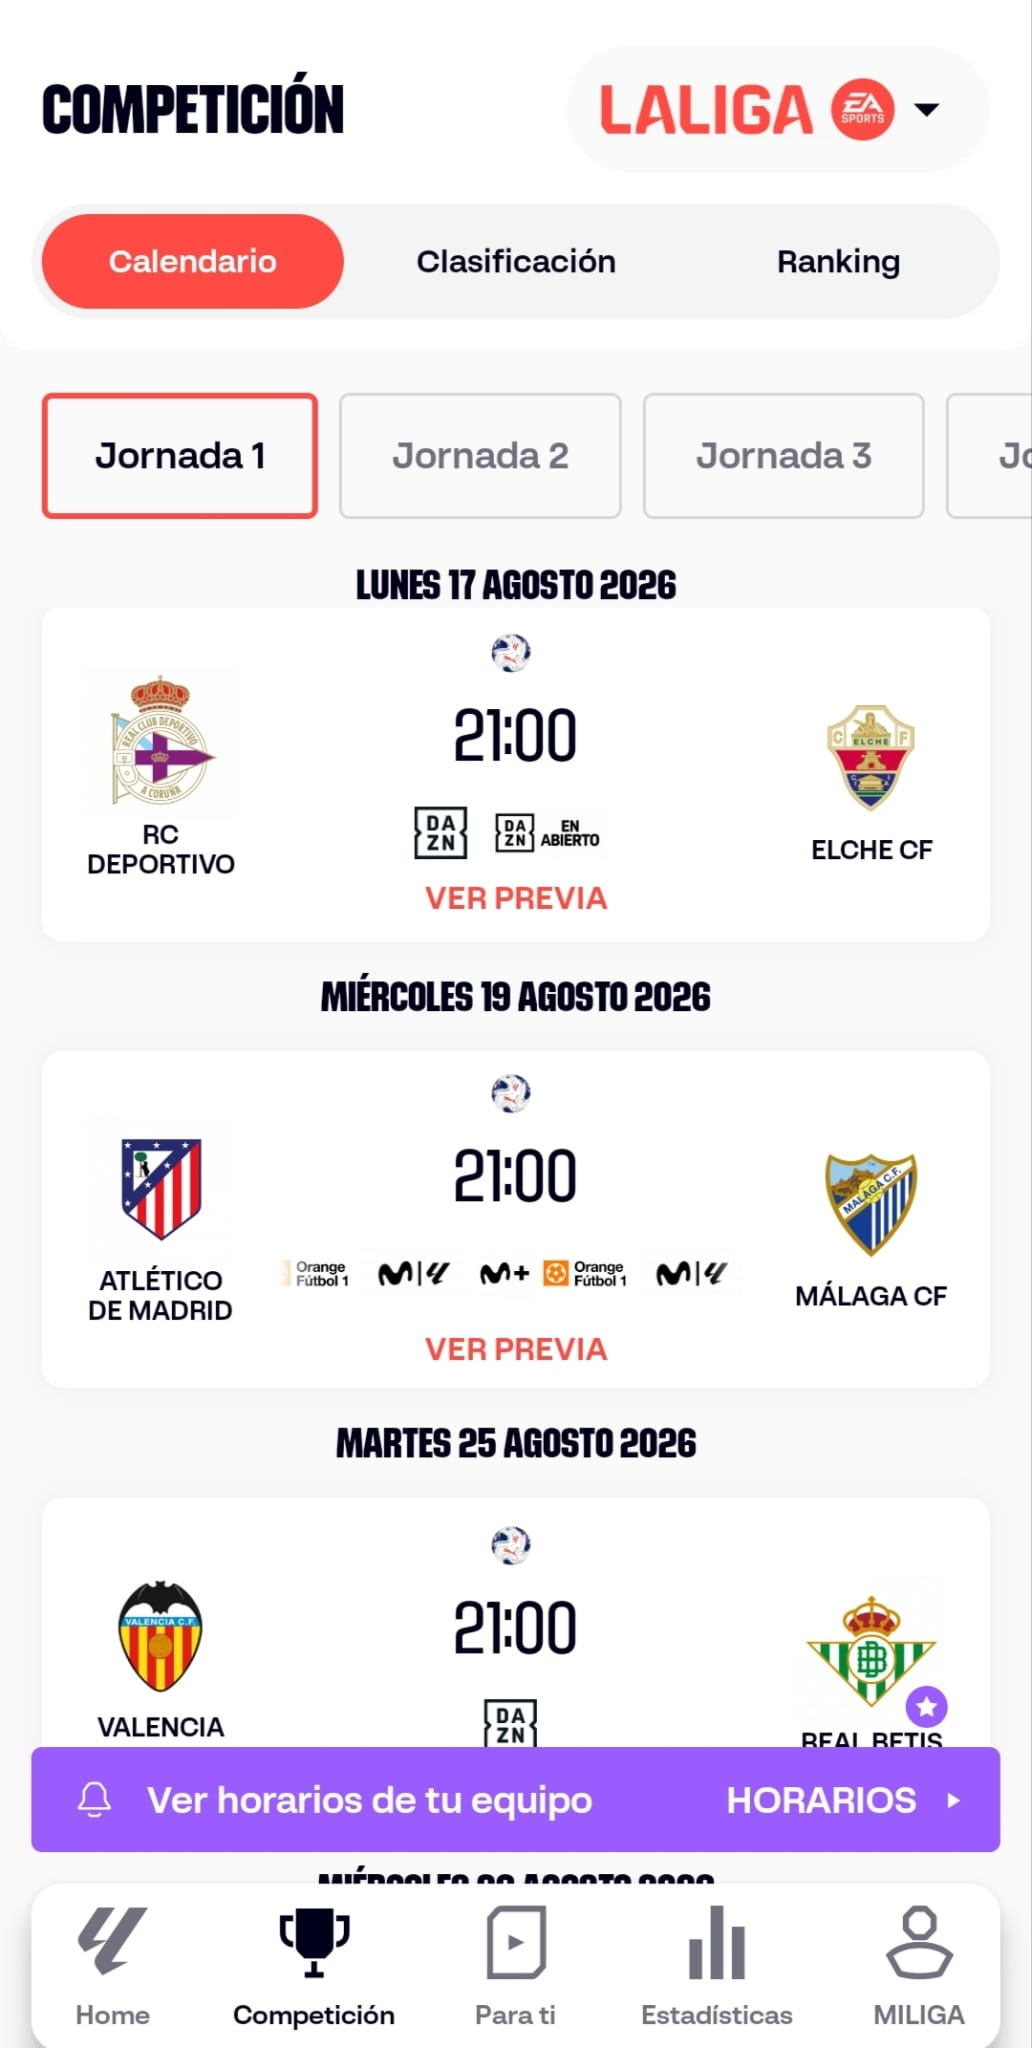
\includegraphics[width=0.5\linewidth]{figures/app_lalila.jpeg}
    \caption{Pantalla de resultados}
    \label{fig:laliga_resultados}
  \end{subfigure}
  \hspace{0.5cm}
  \begin{subfigure}[b]{0.4\textwidth}
    \centering
    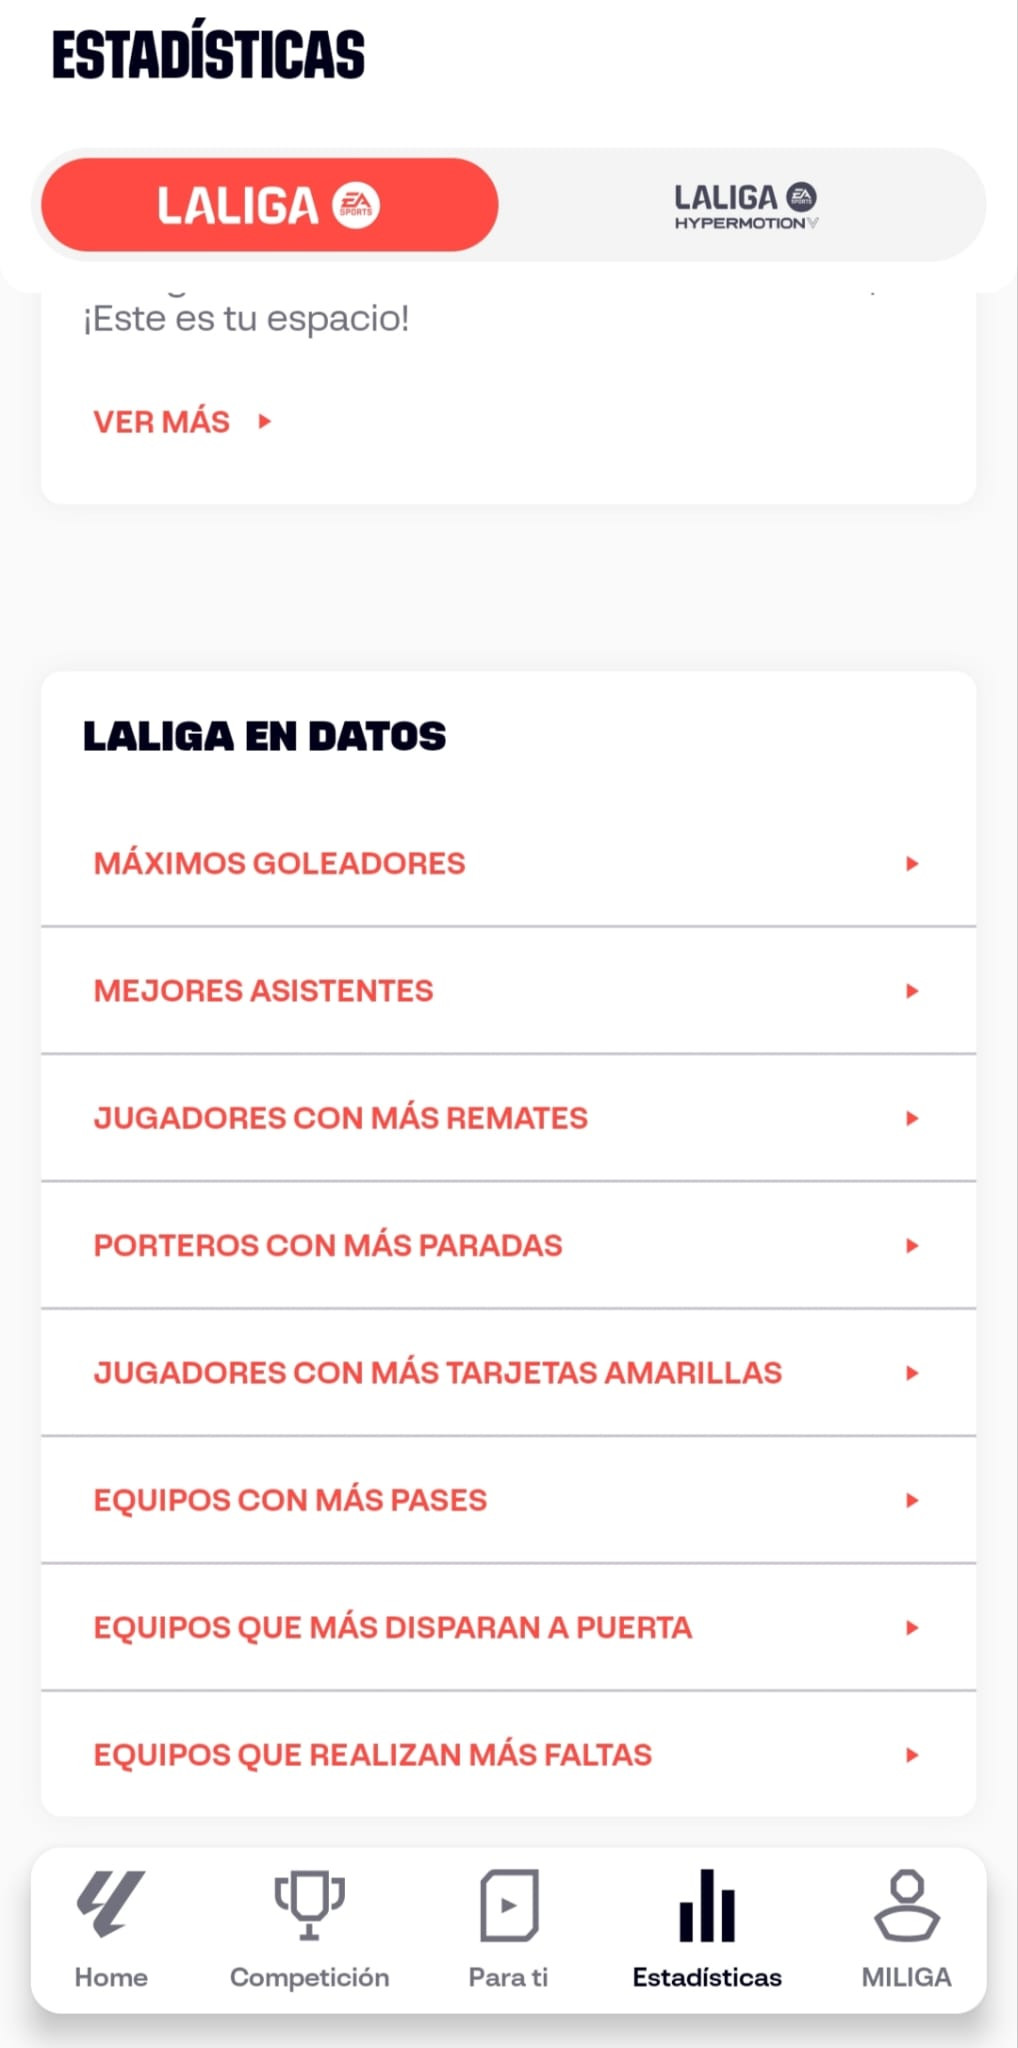
\includegraphics[width=0.5\linewidth]{figures/app_laliga_stats.jpeg}
    \caption{Estadísticas mostradas}
    \label{fig:laliga_stats}
  \end{subfigure}
  \caption{Aplicación oficial de LaLiga}
  \label{fig:laliga}
\end{figure}

\begin{itemize}
    \item BeSoccer: es una aplicación con una cobertura muy amplia, ya que incluye información sobre numerosas ligas y competiciones de fútbol a nivel mundial. Ofrece calendario, clasificaciones, noticias, fichajes, estadísticas de equipos y datos básicos de jugadores. En el apartado de partidos, incorpora información previa como probabilidades, rankings ELO y algunos gráficos comparativos entre equipos, tal y como se muestra en la Figura~\ref{fig:besoccer}.

    Sin embargo, el análisis individual de jugadores es más limitado, ya que se centra principalmente en estadísticas tradicionales como goles, asistencias, tarjetas o partidos disputados. Aunque incluye algunos elementos visuales, como radares de atributos, no siempre se muestra con claridad la base estadística utilizada para construir dichos indicadores. En cuanto al análisis de temporada, destaca la presencia de clasificaciones con probabilidades por rango basadas en simulaciones de Monte Carlo y rankings estadísticos básicos. Por tanto, BeSoccer ofrece una cobertura muy completa, pero su análisis avanzado queda centrado principalmente en determinadas secciones y no se presenta como una herramienta integral de minería de datos.
\end{itemize}

\begin{figure}[H]
\centering
  \begin{subfigure}[b]{0.4\textwidth}
    \centering
    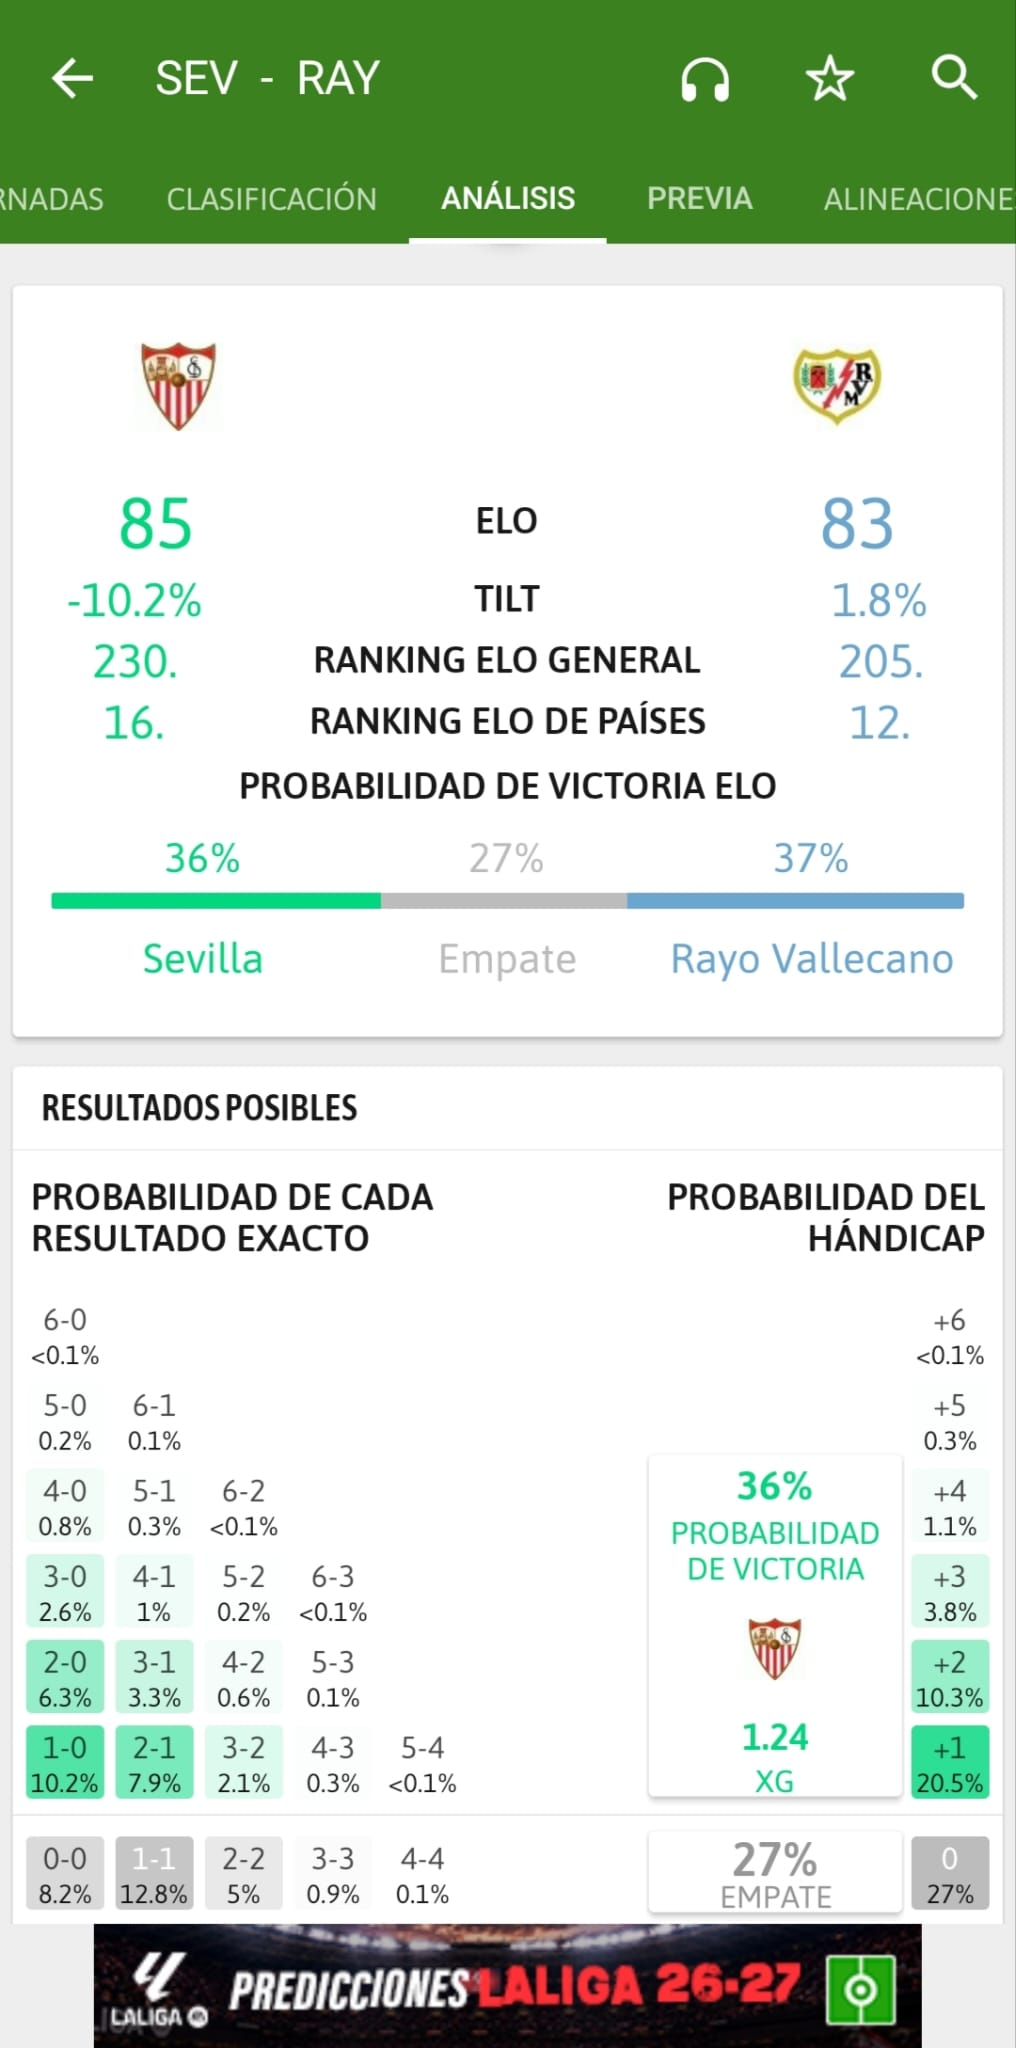
\includegraphics[width=0.5\linewidth]{figures/app_besoccer_prob.jpeg}
    \caption{Pantalla de probabilidades}
    \label{fig:besoccer_prob}
  \end{subfigure}
  \caption{BeSoccer}
  \label{fig:besoccer}
\end{figure}

\begin{itemize}
    \item SofaScore: es probablemente la aplicación más avanzada de las tres en cuanto a volumen de información y nivel estadístico. Su alcance no se limita al fútbol, sino que abarca numerosos deportes y competiciones. En el caso del fútbol, ofrece estadísticas detalladas de partidos, mapas de calor, valoraciones individuales de jugadores, datos de rendimiento y comparativas avanzadas.

    Uno de sus elementos más destacados es el sistema de valoración individual de jugadores, que permite evaluar el rendimiento de cada futbolista en un partido concreto. Como se aprecia en la Figura~\ref{fig:sofascore}, SofaScore ofrece una mayor profundidad estadística que las aplicaciones anteriores. No obstante, parte de sus funcionalidades más avanzadas, especialmente aquellas relacionadas con inteligencia artificial, se encuentran asociadas a servicios de pago. Además, una parte importante de sus análisis previos está orientada al contexto de las apuestas deportivas, lo que puede alejarse del enfoque puramente analítico y académico que persigue este proyecto. A pesar de ello, SofaScore constituye una referencia clara en cuanto a visualización de datos deportivos y profundidad estadística.
\end{itemize}

\begin{figure}[H]
\centering
  \begin{subfigure}[b]{0.4\textwidth}
    \centering
    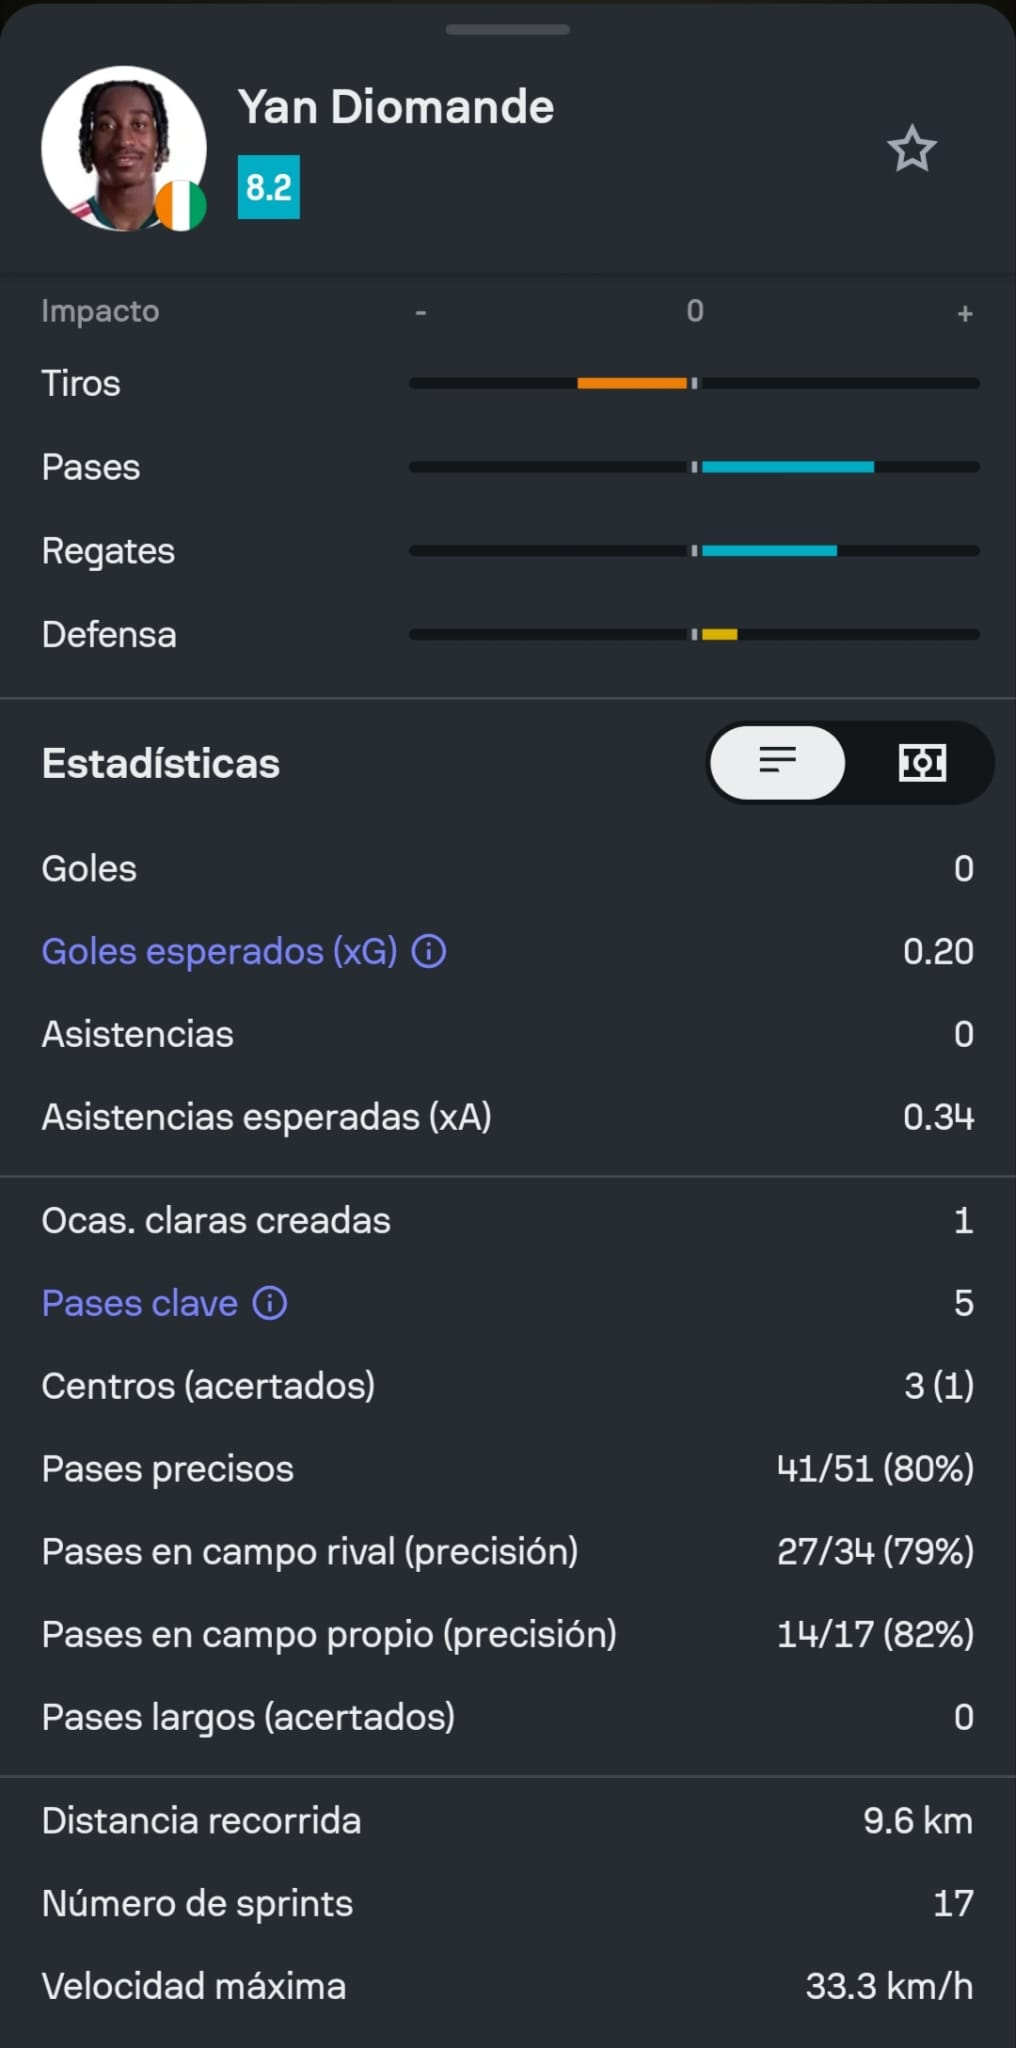
\includegraphics[width=0.5\linewidth]{figures/app_sofascore_stats.jpeg}
    \caption{Estadísticas mostradas}
    \label{fig:sofascore_stats}
  \end{subfigure}
  \hspace{0.5cm}
  \begin{subfigure}[b]{0.4\textwidth}
    \centering
    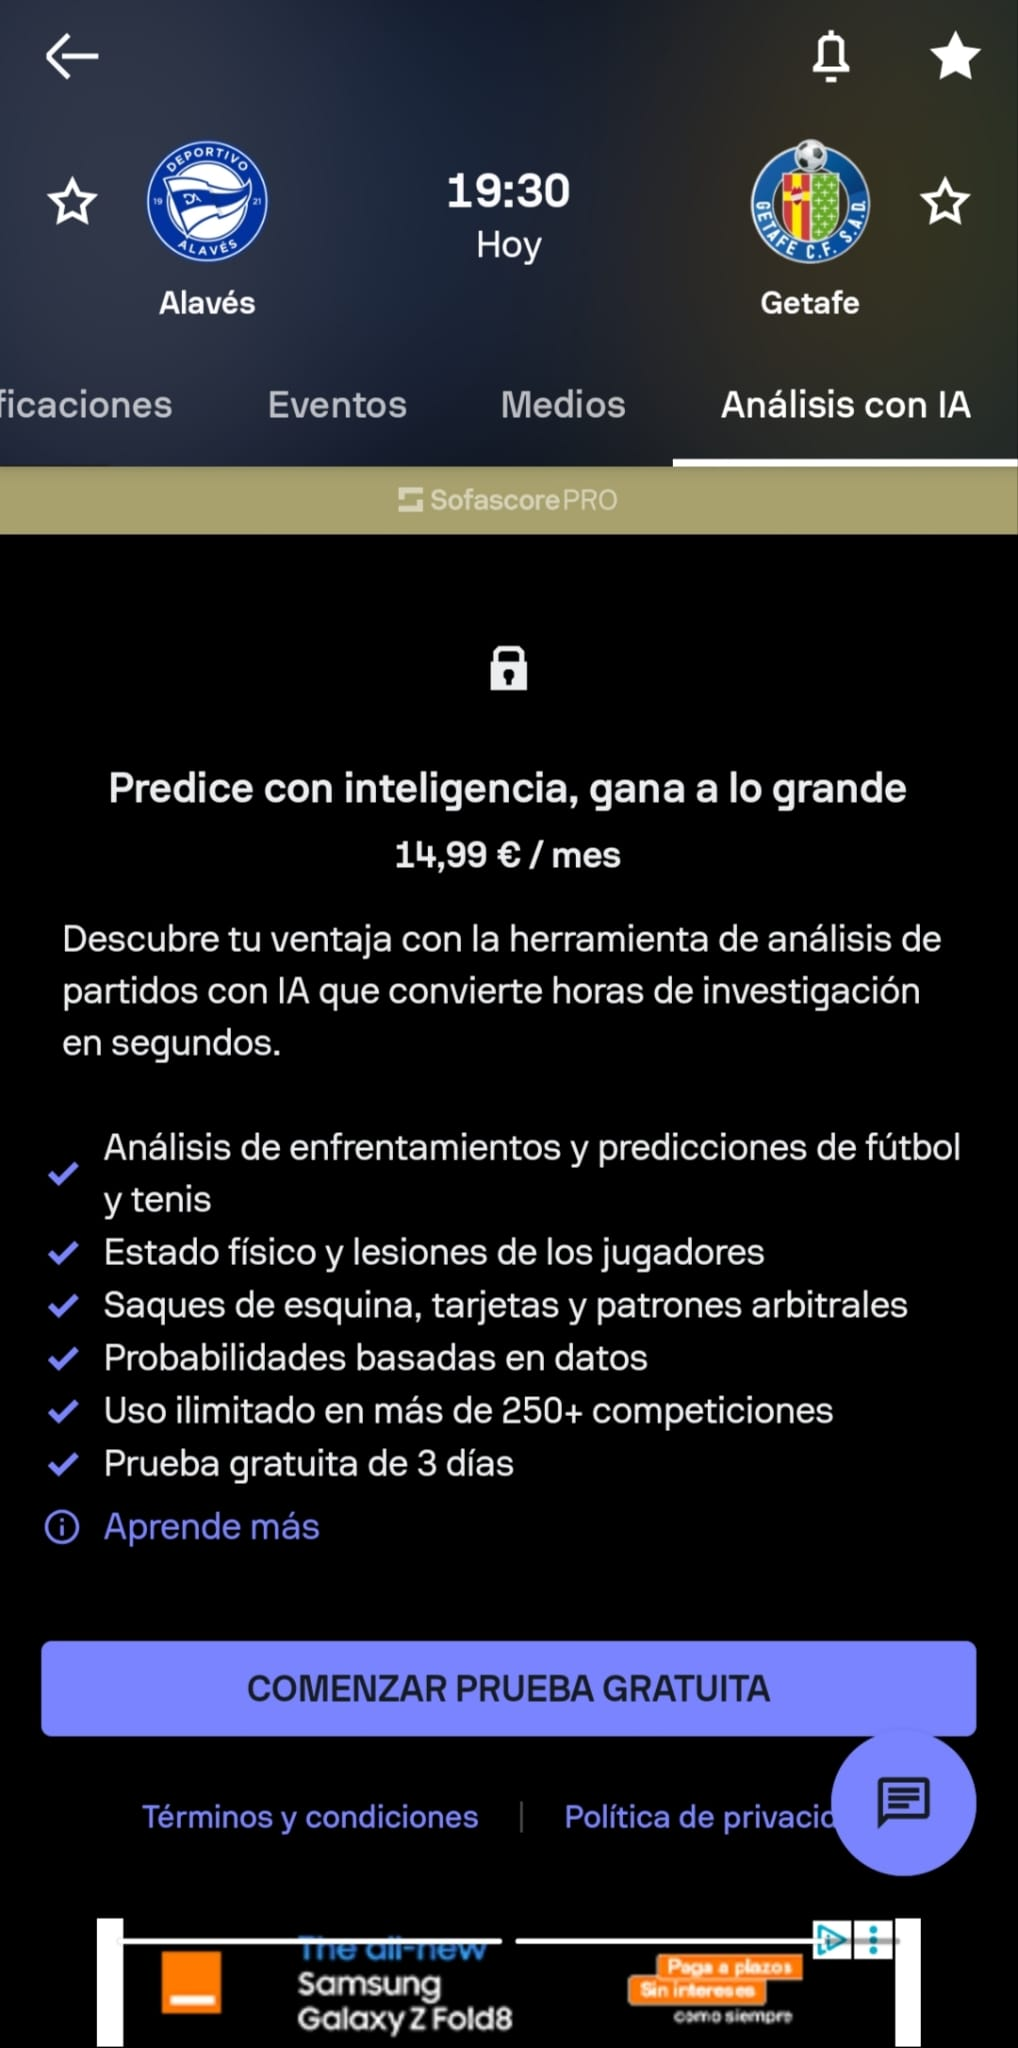
\includegraphics[width=0.5\linewidth]{figures/app_sofasocore_pago.jpeg}
    \caption{Funcionalidades de IA de pago}
    \label{fig:sofascore_ia}
  \end{subfigure}
  \caption{SofaScore}
  \label{fig:sofascore}
\end{figure}

\begin{table}[H]
\centering
\caption{Comparativa de funcionalidades entre aplicaciones de análisis de fútbol.}
\label{tab:comparativa_apps}
\renewcommand{\arraystretch}{1.2}

\begin{tabularx}{\textwidth}{|X|c|c|c|c|}
\hline
\textbf{Característica} & \textbf{BeSoccer} & \textbf{SofaScore} & \textbf{LaLiga} & \textbf{Propuesta} \\ \hline

Estadísticas históricas & \ding{51} & \ding{51} & \ding{51} & \ding{51} \\ \hline

Estadísticas avanzadas & Parcial & Sí & Parcial & \ding{51} \\ \hline

\textit{Dashboards} de \textit{business intelligence} & \ding{55} & \ding{55} & \ding{55} & \ding{51} \\ \hline

Análisis IA Gratis & \ding{51} & Básico & \ding{55} & \ding{51} \\ \hline

Predicción mediante IA & \ding{51} & Parcial & \ding{55} & \ding{51} \\ \hline

Simulación Monte Carlo & \ding{51} & \ding{55} & \ding{55} & \ding{51} \\ \hline

\textit{Clustering} de jugadores & \ding{55} & \ding{55} & \ding{55} & \ding{51} \\ \hline

Detección de necesidades de plantilla & \ding{55} & \ding{55} & \ding{55} & \ding{51} \\ \hline

Chatbot basado en IA & \ding{55} & \ding{55} & \ding{55} & \ding{51} \\ \hline

Simulación interactiva de temporada & \ding{55} & \ding{55} & \ding{55} & \ding{51} \\ \hline

Resultados en directo & \ding{51} & \ding{51} & \ding{51} & \ding{55} \\ \hline
\end{tabularx}
\end{table}



\newpage{\ }
\cleardoublepage

\chapter{Plan de gestión de proyecto}
\label{cap:planificación}
En esta sección se describen todos los aspectos relativos a la gestión del proyecto: metodología, organización, costes, planificación y riesgos de la calidad.

\section{Metodología de desarrollo}

Para el desarrollo de este proyecto se ha adoptado una metodología de desarrollo en cascada con iteraciones (véase Figura~\ref{fig:cascada}). Este enfoque permite seguir una planificación estructurada mediante fases claramente diferenciadas, sin renunciar a la posibilidad de realizar revisiones y mejoras continuas cuando aparecen nuevos requisitos, se detectan errores o surgen oportunidades de optimización. De esta forma, aunque el desarrollo avanza de manera secuencial, es posible regresar a fases anteriores para llevar a cabo ajustes, garantizando una mayor calidad del producto final.

Las principales fases seguidas durante el desarrollo del proyecto han sido las siguientes:

\begin{itemize}
    \item {Inicio:} definición de los objetivos del Trabajo Fin de Grado, estudio de la viabilidad del proyecto y planificación inicial de las tareas a desarrollar, así como selección de las tecnologías más adecuadas.

    \item {Análisis de requisitos:} identificación de los requisitos funcionales y no funcionales de la aplicación, estudio de aplicaciones similares y definición de las funcionalidades que formarían parte del sistema.

    \item {Diseño:} diseño de la arquitectura de \textit{software}, del modelo de datos del \textit{data warehouse}, de la estructura de la base de datos, de la interfaz de usuario y de los algoritmos de minería de datos que se integrarían en la aplicación.

    \item {Construcción:} implementación de todos los componentes del sistema, incluyendo el proceso ETL para la obtención de datos, el desarrollo del \textit{backend} y la API REST, la aplicación móvil en React Native, el \textit{data warehouse}, los algoritmos de análisis de datos y las funcionalidades basadas en inteligencia artificial.

    \item {Integración y pruebas:} integración progresiva de todos los módulos desarrollados y realización de pruebas funcionales para verificar el correcto funcionamiento de la aplicación, detectar posibles errores y validar los resultados obtenidos por los algoritmos implementados.

    \item {Cierre:} elaboración de la documentación técnica y de usuario, revisión final del sistema, optimización del código desarrollado y preparación de la memoria y la defensa del Trabajo Fin de Grado.
\end{itemize}
\begin{figure}
    \centering
    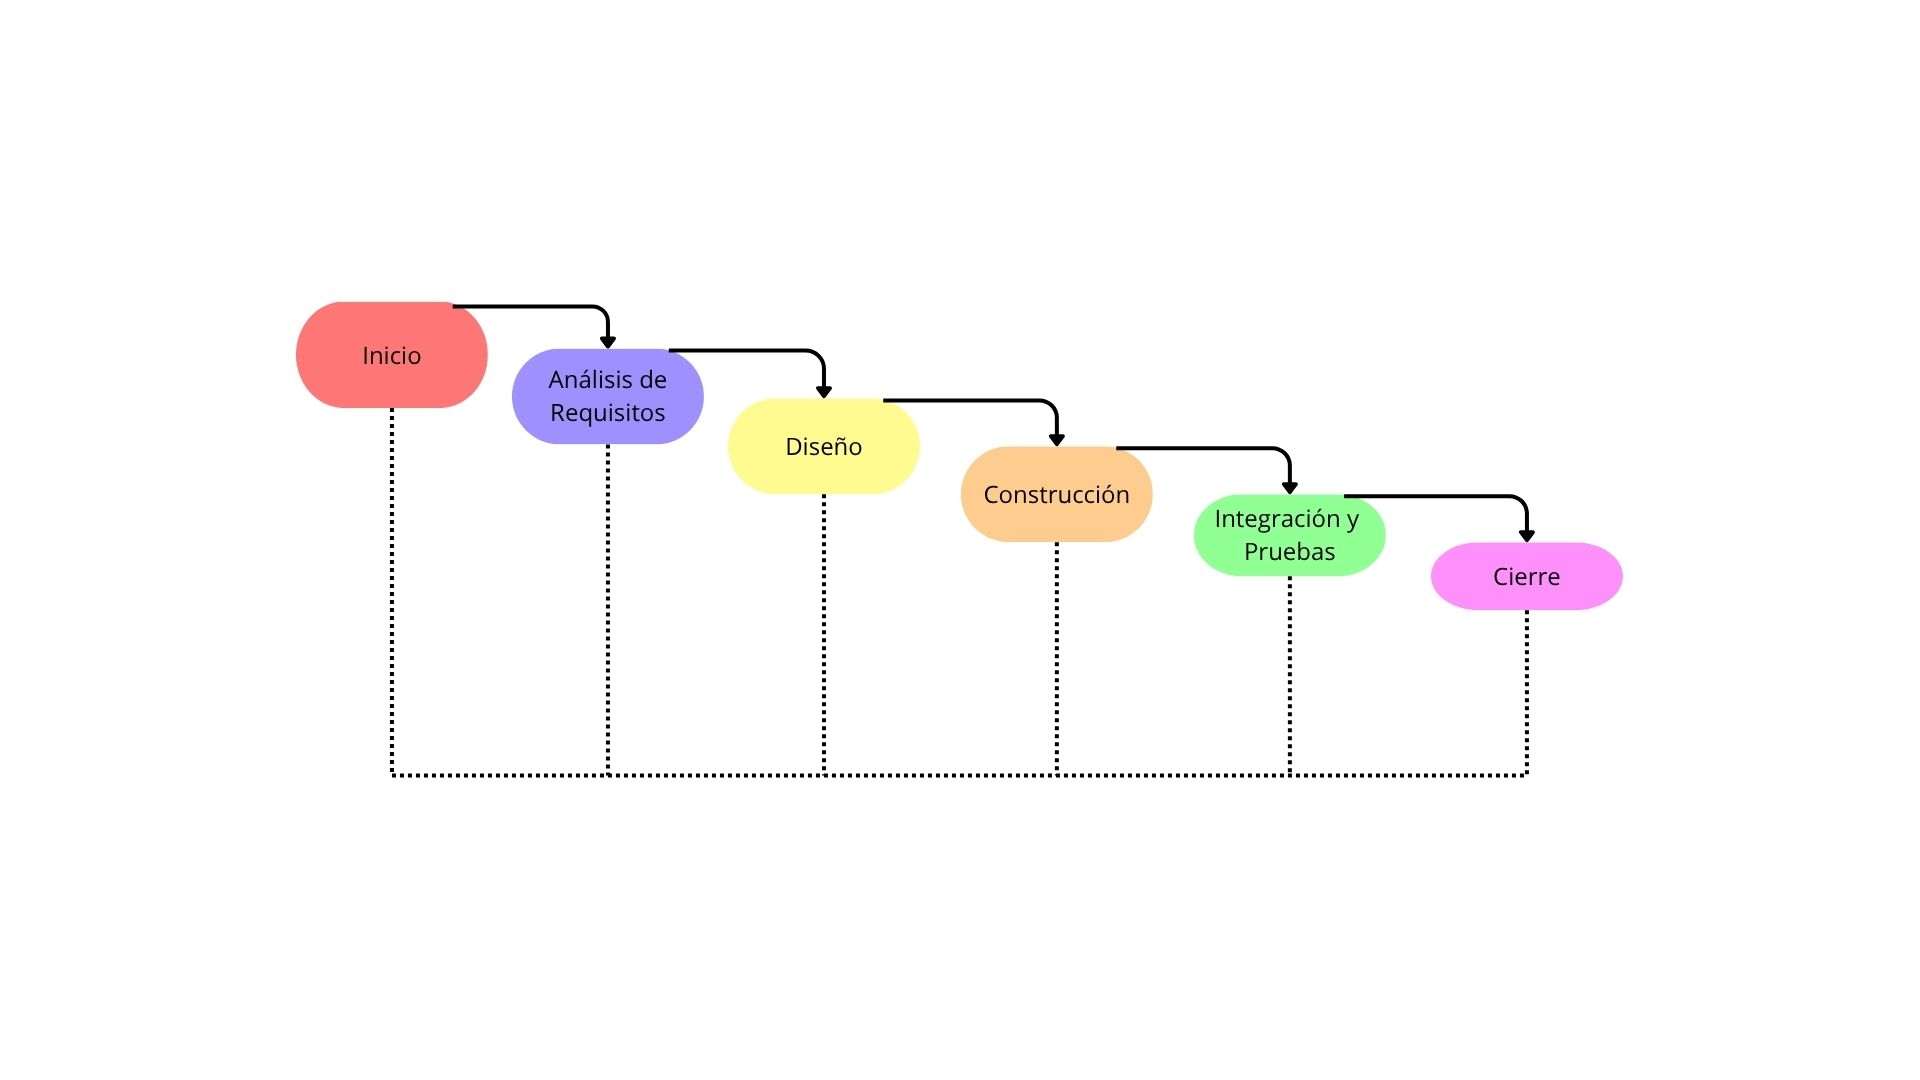
\includegraphics[width=1\linewidth]{figures/metodologia_desarrollo.jpg}
    \caption{Cascada iterativa (creación propia).}
    \label{fig:cascada}
\end{figure}


\section{Tecnologías}

Para este proyecto, se ha decidido hacer una aplicación multiplataforma, ya que se considera que al ser una aplicación dedicada tanto a aficionados como a analistas profesionales, era una buena práctica ofrecer al usuario una experiencia dedicada a su campo; si es un aficionado, la usará más en móvil, y si es un profesional, en ordenador. Además, el \textit{framework} usado nos permite implementar tanto para Android como para iOS con facilidad, así que también tendremos ese añadido.

En cuanto al diseño de la aplicación, podemos diferenciar \textit{frontend} y \textit{backend}. Además, se usa una tecnología como GitHub y GitHub Desktop, que nos permiten tener un control de versiones de la manera más eficiente y nos facilitan el desarrollo del proyecto y de sus cambios.

\subsection{\textit{Frontend}}

Para el desarrollo de la aplicación móvil se han tenido en cuenta tres tecnologías principales: Kotlin, React Native y Flutter. Todas ellas permiten desarrollar aplicaciones para dispositivos móviles, aunque presentan diferencias en cuanto a lenguaje utilizado, facilidad de desarrollo, rendimiento y experiencia previa del desarrollador.

En primer lugar, se valoró el uso de Kotlin. Kotlin es un lenguaje de programación moderno, conciso y de código abierto, desarrollado por \textit{JetBrains}, optimizado para la JVM, Android y el desarrollo multiplataforma. Destaca por su interoperabilidad con Java, su tipado estático, la seguridad frente a valores nulos y el soporte tanto para programación funcional como orientada a objetos. Aunque se contaba con experiencia previa en este lenguaje, los problemas de rendimiento encontrados con el emulador hicieron que se exploraran otras alternativas.

Otra opción considerada fue React Native. React Native es un \textit{framework} de código abierto creado por \textit{Facebook} para el desarrollo de aplicaciones móviles nativas para iOS y Android utilizando JavaScript y React. Esta opción resultaba especialmente atractiva al basarse en JavaScript, un lenguaje ya utilizado en proyectos anteriores, además de ser una tecnología ampliamente utilizada en el ámbito del desarrollo móvil.

Por último, también se tuvo en cuenta Flutter. Flutter es un \textit{framework} de código abierto desarrollado por \textit{Google} que permite crear aplicaciones compiladas de forma nativa y de alto rendimiento para dispositivos móviles, web y escritorio a partir de una única base de código. Se consideró una alternativa interesante por su enfoque multiplataforma, su rendimiento y su buena gestión de interfaces gráficas.

Finalmente, se decidió desarrollar la aplicación con React Native debido a la experiencia previa con JavaScript, la facilidad para realizar despliegues multiplataforma, la posibilidad de visualizar cambios en tiempo real durante el desarrollo y su alta demanda en el mercado laboral.

\subsection{\textit{Backend}}
Para la parte destinada a gestionar las peticiones que podrá realizar el usuario, se ha decidido emplear un conjunto de tecnologías que garanticen la persistencia, seguridad y eficiencia en el manejo de grandes volúmenes de datos.

\subsubsection{Base de datos}
Para la elección de la base de datos, primero se analizaron los dos paradigmas principales existentes en la actualidad: las bases de datos relacionales y las no relacionales (NoSQL).

Las bases de datos NoSQL ofrecen una gran flexibilidad y escalabilidad horizontal; sin embargo, para este proyecto se ha optado por una base de datos relacional. Esta decisión se basa en que los datos deportivos (jugadores, equipos, partidos y estadísticas) presentan una estructura tabular clara y relaciones estrictas entre ellos. El modelo relacional permite garantizar la integridad referencial mediante el uso de claves foráneas, asegurando que cada estadística esté correctamente vinculada a un jugador y un partido existentes, evitando así inconsistencias que podrían falsear los análisis posteriores.

\subsubsection{SGBD}
Como sistema gestor de bases de datos (SGBD) se ha seleccionado PostgreSQL. 

PostgreSQL es un sistema de código abierto objeto-relacional que destaca por su robustez, fiabilidad y por cumplir estrictamente con los estándares SQL. Su naturaleza \textit{open source} lo convierte en una opción idónea para proyectos académicos como el presente, ofreciendo prestaciones de nivel empresarial sin incurrir en costes de licenciamiento.

Para la administración y gestión de la base de datos se utilizará DBeaver. Esta herramienta de gestión universal permite interactuar con el servidor de forma visual y sencilla, facilitando tareas como la ejecución de consultas, el diseño de diagramas entidad-relación y la monitorización de los datos de manera intuitiva.

Durante la fase de planificación se consideraron otras alternativas, siendo MySQL la opción más destacada. Si bien MySQL es un gestor ampliamente utilizado, se eligió PostgreSQL debido a la experiencia previa en otros proyectos y, fundamentalmente, por las funciones avanzadas que ofrece este último (como su potencia en consultas analíticas), las cuales se adaptan mejor a los requisitos de procesamiento de datos de este trabajo.
\subsubsection{API}

Además de la base de datos y del SGBD, la aplicación necesita una API que sea capaz de gestionar las peticiones realizadas desde la aplicación móvil y proporcionar la funcionalidad necesaria sobre los datos almacenados. Para esta parte del sistema existen distintas tecnologías disponibles, aunque en este proyecto se han tenido en cuenta principalmente dos alternativas: Node.js y Python mediante FastAPI.

En primer lugar, una de las opciones consideradas ha sido Node.js. Node.js es un entorno de ejecución para JavaScript que permite ejecutar este lenguaje en el servidor, fuera del navegador. Está basado en el motor V8 de Google Chrome y destaca por su modelo de entrada/salida no bloqueante y orientado a eventos, lo cual lo hace adecuado para aplicaciones que requieren manejar varias conexiones al mismo tiempo, como \textit{chats}, APIs REST y servicios en tiempo real.

Por otro lado, también se ha valorado el uso de Python junto con FastAPI. Python es un lenguaje de programación interpretado, de alto nivel, conocido por su sintaxis clara y su legibilidad. En el desarrollo de APIs, Python es muy valorado por permitir escribir código rápidamente y con pocos errores, lo que lo hace adecuado para prototipado, ciencia de datos y aplicaciones basadas en inteligencia artificial. Para construir APIs en Python, uno de los \textit{frameworks} más utilizados actualmente es FastAPI.

Tras analizar ambas alternativas, se ha decidido utilizar Node.js, debido a que el desarrollador ya cuenta con experiencia previa en su uso dentro de otros proyectos académicos relacionados con la construcción de APIs. Además, al desarrollarse la aplicación móvil con React Native, el uso de Node.js en el \textit{backend} permite mantener una mayor coherencia en el lenguaje de programación empleado en el proyecto. Esto facilita la reutilización de conocimientos y agiliza el desarrollo al no tener que alternar entre diferentes sintaxis.

\subsubsection{Proceso ETL y \textit{data mining}}

Para la fase de procesamiento de datos y extracción de conocimiento, se ha seleccionado Python como lenguaje principal, debido a su versatilidad y a su ecosistema de librerías especializadas en ciencia de datos. Esta parte del sistema se divide en dos etapas fundamentales: el proceso ETL y la posterior aplicación de técnicas de \textit{data mining}.

En primer lugar, el proceso ETL (\textit{Extract, Transform, Load}) se encarga de preparar los datos antes de su carga definitiva en la base de datos. En esta fase se han desarrollado \textit{scripts} personalizados para la extracción de los datos en formato JSON procedentes de la API deportiva. Utilizando la librería Pandas, se realiza la limpieza y transformación de los datos, incluyendo la normalización de estructuras anidadas, la gestión de valores nulos y la corrección de tipos de datos, como la conversión de decimales innecesarios a enteros. Finalmente, los datos procesados se cargan de forma estructurada en la base de datos PostgreSQL.

Una vez consolidada la base de datos, se desarrolla la fase de \textit{data mining}. En esta etapa se aplican técnicas de minería de datos para descubrir patrones en el rendimiento de jugadores y equipos, generar indicadores y realizar predicciones. Python facilita la implementación de algoritmos de aprendizaje automático y análisis estadístico, permitiendo transformar los datos brutos en información de valor para el análisis deportivo.

La elección de Python se justifica por la potencia de herramientas como Pandas para la manipulación de grandes volúmenes de datos y Psycopg2 para la conexión eficiente con el servidor PostgreSQL.

\subsubsection{Asistente conversacional}

Para la implementación del asistente conversacional de la aplicación se ha utilizado Gemini, un modelo de inteligencia artificial generativa desarrollado por Google. Esta tecnología permite interpretar preguntas realizadas en lenguaje natural por el usuario y transformarlas en consultas sobre la información almacenada en el sistema.

El uso de Gemini se justifica por la necesidad de ofrecer una forma de consulta más flexible e intuitiva que la navegación tradicional por pantallas. A través del asistente, denominado Agente de oro, el usuario puede preguntar por estadísticas de jugadores, equipos, partidos o temporadas sin tener que acceder manualmente a cada apartado de la aplicación.

La integración se realiza desde el \textit{backend}, que actúa como intermediario entre la aplicación móvil, la base de datos y el modelo de inteligencia artificial. De esta forma, el usuario no interactúa directamente con el servicio externo, sino que las peticiones son controladas por la API, permitiendo limitar el tipo de consultas permitidas y garantizar que las respuestas se basen únicamente en la información deportiva disponible en la base de datos.

\subsubsection{Contenedorización y despliegue}

Para facilitar la ejecución del sistema en distintos entornos se ha considerado el uso de Docker. Docker permite empaquetar los diferentes servicios de la aplicación en contenedores independientes, asegurando que el backend, la base de datos y el resto de componentes se ejecuten con una configuración controlada y reproducible.

En este proyecto, la contenedorización resulta especialmente útil para simplificar la puesta en marcha del entorno de desarrollo y evitar problemas derivados de diferencias entre sistemas operativos, versiones de dependencias o configuraciones locales. Mediante un archivo de composición de servicios, es posible definir la base de datos PostgreSQL, el servidor backend y las variables de entorno necesarias para que la aplicación pueda ejecutarse de forma más sencilla en otra máquina.

Aunque el despliegue final en producción queda fuera del alcance principal del Trabajo Fin de Grado, Docker proporciona una base adecuada para una futura publicación del sistema, ya que permitiría trasladar el backend y la base de datos a un servidor externo manteniendo una configuración similar a la utilizada durante el desarrollo.

\section{Planificación del proyecto}
El diagrama de Gantt de la figura~\ref{fig:gantt} muestra el tiempo dedicado a desarrollar las diferentes partes del proyecto, empezando por el análisis de datos, diseño, implementación de arquitectura y aplicación, y acabando por la memoria. 
\begin{figure}[H]
    \centering
    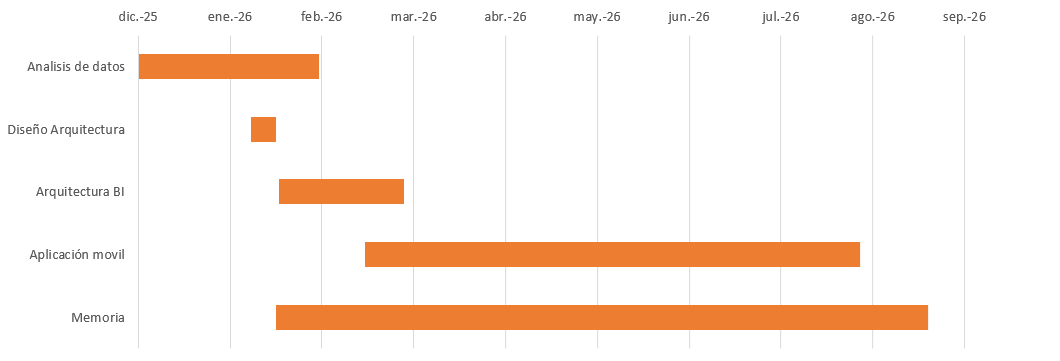
\includegraphics[width=1\linewidth]{figures/gantt_tfg.png}
    \caption{Diagrama de Gantt del proyecto.}
    \label{fig:gantt}
\end{figure}

\section{Costes}

En esta sección se presenta una estimación de los costes asociados al desarrollo del proyecto. Dado que se trata de un Trabajo Fin de Grado, muchos de los recursos utilizados ya estaban disponibles previamente o han sido empleados en un entorno académico, por lo que no todos han supuesto un coste económico directo. No obstante, se incluye una valoración aproximada del esfuerzo humano, los recursos materiales y los posibles costes de servicio en caso de que la aplicación quisiera desplegarse en un entorno de producción.

\subsection{Costes de recursos humanos}

El principal coste del proyecto corresponde al tiempo dedicado al análisis, diseño, desarrollo, pruebas y documentación del sistema. Aunque el trabajo ha sido realizado por un único desarrollador en el contexto académico del Trabajo Fin de Grado, se ha estimado su coste tomando como referencia una tarifa de 15 euros por hora, correspondiente a un perfil de desarrollador junior.

El periodo de desarrollo se ha extendido aproximadamente desde febrero hasta septiembre. Durante este periodo se estima que se ha trabajado en torno al 75 \% de los días, con una dedicación media aproximada de dos horas diarias. A partir de esta estimación, se obtiene un total de 363 horas de trabajo.

La Tabla~\ref{tab:costes_recursos_humanos} resume el coste estimado asociado a los recursos humanos.

\begin{table}[H]
\centering
\caption{Costes de recursos humanos.}
\label{tab:costes_recursos_humanos}
\renewcommand{\arraystretch}{1.2}
\begin{tabular}{|p{5cm}|p{4cm}|p{4cm}|}
\hline
\textbf{Concepto} & \textbf{Cantidad} & \textbf{Coste estimado} \\ \hline

Periodo de desarrollo &
Febrero - septiembre &
- \\ \hline

Dedicación estimada &
363 horas &
- \\ \hline

Coste por hora &
15 \euro/hora &
- \\ \hline

Desarrollo del proyecto &
363 horas &
5.445 \euro \\ \hline

\textbf{Total recursos humanos} &
&
\textbf{5.445 \euro} \\ \hline

\end{tabular}
\end{table}

\subsection{Costes materiales}

Los costes materiales corresponden a los recursos físicos y de soporte utilizados durante el desarrollo del proyecto. En este caso, se ha utilizado un ordenador portátil personal y un dispositivo móvil físico para realizar pruebas de la aplicación. Al tratarse de recursos ya disponibles antes del inicio del proyecto, no se ha imputado un coste directo asociado a su adquisición.

Además, se han considerado otros recursos necesarios para el desarrollo, como la conexión a Internet y el consumo eléctrico. Aunque estos recursos forman parte del entorno doméstico habitual, se incluye una estimación proporcional asociada al tiempo dedicado al proyecto. Para la electricidad, se ha estimado el consumo aproximado del ordenador portátil durante las horas de trabajo. Para la conexión a Internet, se ha considerado una parte proporcional del uso durante los meses de desarrollo.

La Tabla~\ref{tab:costes_materiales} recoge los principales costes materiales considerados.

\begin{table}[H]
\centering
\caption{Costes materiales.}
\label{tab:costes_materiales}
\renewcommand{\arraystretch}{1.2}
\begin{tabular}{|p{6cm}|p{5cm}|p{3cm}|}
\hline
\textbf{Recurso} & \textbf{Descripción} & \textbf{Coste} \\ \hline

Ordenador portátil &
Recurso personal ya disponible &
0 \euro \\ \hline

Dispositivo móvil &
Recurso personal utilizado para pruebas &
0 \euro \\ \hline

Conexión a Internet &
Uso proporcional de la red doméstica durante el desarrollo del proyecto &
40 \euro \\ \hline

Consumo eléctrico &
Estimación del consumo del equipo durante las horas de desarrollo &
5 \euro \\ \hline

\textbf{Total costes materiales} &
&
\textbf{45 \euro} \\ \hline

\end{tabular}
\end{table}

\subsection{Costes de servicios}

Durante el desarrollo del proyecto se ha utilizado la API-Football durante un mes para obtener datos históricos y actuales de la competición. Este servicio ha supuesto un coste directo de 30 euros. Por otro lado, el asistente inteligente se ha apoyado en Google AI Studio, disponible de forma gratuita mediante el entorno universitario, por lo que no se ha considerado coste asociado a este servicio dentro del desarrollo académico.

La Tabla~\ref{tab:costes_servicios_desarrollo} muestra los costes de servicios utilizados durante el desarrollo.

\begin{table}[H]
\centering
\caption{Costes de servicios durante el desarrollo.}
\label{tab:costes_servicios_desarrollo}
\renewcommand{\arraystretch}{1.2}
\begin{tabular}{|p{6cm}|p{6cm}|p{3cm}|}
\hline
\textbf{Servicio} & \textbf{Uso en el proyecto} & \textbf{Coste} \\ \hline

API-Football &
Obtención de datos históricos y actuales de LaLiga durante un mes &
30 \euro \\ \hline

Google AI Studio &
Servicio utilizado para el asistente conversacional en entorno académico &
0 \euro \\ \hline

\textbf{Total servicios de desarrollo} &
&
\textbf{30 \euro} \\ \hline

\end{tabular}
\end{table}

Además de los costes reales del desarrollo, se puede considerar un escenario hipotético de puesta en producción. En dicho caso, la aplicación requeriría una infraestructura adicional para alojar el backend, la base de datos, los servicios de inteligencia artificial y el consumo recurrente de una API deportiva. Estos costes no forman parte del coste real del Trabajo Fin de Grado, pero permiten estimar la inversión necesaria si el sistema quisiera desplegarse para usuarios reales.

La Tabla~\ref{tab:costes_produccion} presenta una estimación mensual para un posible despliegue en producción.

\begin{table}[H]
\centering
\caption{Estimación de costes mensuales en un escenario de producción.}
\label{tab:costes_produccion}
\renewcommand{\arraystretch}{1.2}
\begin{tabular}{|p{6cm}|p{6cm}|p{3cm}|}
\hline
\textbf{Servicio} & \textbf{Descripción} & \textbf{Coste mensual estimado} \\ \hline

Servidor backend &
Alojamiento de la API REST desarrollada en Node.js &
10--20 \euro \\ \hline

Base de datos PostgreSQL &
Servicio gestionado o servidor con PostgreSQL desplegado &
15--30 \euro \\ \hline

API de datos deportivos &
Obtención periódica o en tiempo real de datos de partidos, equipos y jugadores &
30--100 \euro \\ \hline

Servicio de inteligencia artificial &
Uso de un modelo de lenguaje para el asistente conversacional &
0--30 \euro \\ \hline

Dominio y certificado SSL &
Dominio web y seguridad HTTPS básica &
1--5 \euro \\ \hline

Monitorización y copias de seguridad &
Control básico del estado del sistema y respaldo de datos &
5--15 \euro \\ \hline

\textbf{Total mensual estimado} &
&
\textbf{61--200 \euro/mes} \\ \hline

\end{tabular}
\end{table}

Esta estimación dependería del número de usuarios, la frecuencia de actualización de los datos, el volumen de consultas realizadas al asistente inteligente y el nivel de disponibilidad requerido. Por tanto, debe entenderse como una aproximación inicial para un despliegue básico, no como un presupuesto cerrado de explotación comercial.

\subsection{Coste total estimado}

Teniendo en cuenta los costes reales asociados al desarrollo académico del proyecto, el coste total estimado se obtiene sumando el coste de recursos humanos, los costes materiales y los servicios utilizados durante el desarrollo.

La Tabla~\ref{tab:coste_total_proyecto} recoge el coste total estimado del proyecto.

\begin{table}[H]
\centering
\caption{Coste total estimado del proyecto.}
\label{tab:coste_total_proyecto}
\renewcommand{\arraystretch}{1.2}
\begin{tabular}{|p{8cm}|p{4cm}|}
\hline
\textbf{Concepto} & \textbf{Coste} \\ \hline

Costes de recursos humanos &
5.445 \euro \\ \hline

Costes materiales &
45 \euro \\ \hline

Costes de servicios durante el desarrollo &
30 \euro \\ \hline

\textbf{Coste total estimado del proyecto} &
\textbf{5.520 \euro} \\ \hline

\end{tabular}
\end{table}

Por tanto, el coste estimado del desarrollo del proyecto asciende a 5.520 euros. Este valor representa una estimación económica del esfuerzo y los recursos empleados durante el Trabajo Fin de Grado, aunque el coste real asumido ha sido menor al haberse utilizado principalmente recursos personales, herramientas gratuitas y servicios académicos.
\section{Riesgos}
Para poder anticipar obstáculos y posibles errores que tengamos que solucionar, es fundamental identificar los posibles riesgos que podamos encontrar por el camino. Estos serían los principales riesgos que podemos encontrar:
\begin{itemize}
    \item Cambios en los requisitos: durante el proceso, podemos encontrar dificultades en algunas funcionalidades o plataformas usadas que pueden desencadenar retrasos o modificaciones.
    \item Curva de aprendizaje: podemos encontrar dificultades para aprender a usar una tecnología o lenguaje que nunca se haya usado, y tener que ralentizar para dominarla.
    \item Rango de datos limitado: por falta de financiación para una API de datos futbolísticos avanzada, quizás los datos recogidos no sean lo más completos posible para hacer los análisis.
    \item \textit{Hardware} y recursos de pruebas: el desarrollo de aplicación móvil conlleva tener un \textit{hardware} que sea capaz de ejecutar la app para la toma de pruebas.
    \item Compatibilidad entre plataformas: podemos tener dificultades en la portabilidad de la aplicación hacia Android o iOS.
\end{itemize}




  
    % DESARROLLO
    \part{Desarrollo}
    \null\vfill

\chapter{Diseño del sistema}

En este capítulo se presentan los objetivos y el catálogo de requisitos del nuevo sistema informático. 

% \section{Objetivos de negocio}
% El propósito de este sistema es transformar grandes volúmenes de datos históricos de la Liga Española (2015-2025) en conocimiento estratégico mediante una plataforma accesible. Los objetivos de negocio son:
% \begin{itemize}
%     \item Accesibilidad a datos históricos y scouting: Proporcionar una app que permita a aficionados y clubes realizar consultas complejas y análisis de rendimiento sin necesidad de conocimientos técnicas.
%     \item Identificación de patrones de éxito: Facilitar el análisis comparativo para determinar qué variables estadísticas (posesión, precisión, recuperaciones) correlacionan más estrechamente con la obtención de puntos y el rendimiento a largo plazo.
%     \item Monitorización de tendencias: Identificar de forma temprana cambios en el estado de forma de los equipos, permitiendo una toma de decisiones reactiva basada en datos actualizados jornada a jornada.
%     \item Descubrimiento de talento mediante similitud: Implementar algoritmos que permitan identificar "jugadores espejo" o perfiles similares basándose en métricas de rendimiento objetivas, superando el análisis subjetivo tradicional.
%     \item Seguimiento de la actualidad: Permitir al aficionado saber cuales son los últimos resultados de cada equipo y cuales serán los próximos que tendrá que jugar.
    
% \end{itemize}
% \section{Objetivos del sistema}
% Desde una perspectiva técnica, el sistema debe cumplir con los siguientes pilares:
% \begin{itemize}
%     \item Pipeline de datos robusto (ETL): Implementar un proceso de Extracción, Transformación y Carga automatizado en Python que gestione la ingesta multitemporada desde APIs externas, garantizando la limpieza y consistencia de los datos.
%     \item Arquitectura de Inteligencia de Negocio: Diseñar un Data Warehouse optimizado para analítica (OLAP) que consolide estadísticas de equipos, jugadores y partidos de una década de competición.
%     \item Motor de Analítica Avanzada: Desarrollar un módulo de Data Mining capaz de calcular índices de rendimiento (Scoring) y realizar agrupamientos (Clustering) de jugadores.
%     \item Interfaz Multiplataforma: Desarrollar una aplicación móvil (Android/iOS y web) intuitiva que permita la visualización dinámica de las analíticas y la simulación jornada a jornada.
% \end{itemize}
\section{Requisitos del sistema}

\subsection{Requisitos funcionales}

Los requisitos funcionales describen las funcionalidades específicas o los servicios que el sistema debe ofrecer.

\begin{itemize}

    \item RF1. Autenticación y control de acceso: el sistema permitirá el acceso mediante credenciales únicas, validando la identidad del usuario contra la base de datos y gestionando el mantenimiento de la sesión activa mediante \textit{tokens} de seguridad.

    \item RF2. Calendario y resultados de competición: el sistema ofrecerá una visualización cronológica de los partidos, permitiendo filtrar por jornada y mostrando el estado de los encuentros y sus resultados de forma actualizada.

    \item RF3. Visualización de datos tabulares: el sistema presentará tablas detalladas de equipos, jugadores y temporadas que permitirán la ordenación y el filtrado por métricas específicas, integrando los datos descriptivos con los analíticos generados.

    \item RF4. Análisis gráfico de rendimiento: el sistema generará representaciones visuales, como gráficos de radar para los perfiles de jugadores y gráficos de líneas para las tendencias, que faciliten la interpretación de los indicadores clave de rendimiento (\textit{KPI}).

    \item RF5. Motor de predicción de resultados: el sistema proporcionará una estimación probabilística del resultado de futuros encuentros basándose en modelos estadísticos y en el estado de forma actual de los contendientes.

    \item RF6. Identificación de jugadores similares: el sistema permitirá seleccionar un jugador y obtener una lista de perfiles similares basada en algoritmos de \textit{clustering}.

    \item RF7. Adaptabilidad de la interfaz (modo oscuro): el sistema permitirá conmutar el esquema de colores de la interfaz entre el modo claro y el modo oscuro, mejorando la accesibilidad y la experiencia de usuario según las condiciones de luminosidad.

    \item RF8. Gestión de preferencias y ajustes: el sistema ofrecerá un panel de configuración en el que el usuario podrá personalizar  los parámetros de visualización por defecto.

    \item RF9. Gestión de la cuenta de usuario: el sistema permitirá al usuario modificar sus datos personales, actualizar la contraseña de acceso y ejercer su derecho de supresión de la cuenta y eliminación de sus datos.

    \item RF10. Sistema de seguimiento de favoritos: el sistema permitirá marcar jugadores o equipos como favoritos para obtener acceso directo a sus estadísticas.

    \item RF11. Comparador directo (\textit{Head-to-Head}): el sistema permitirá seleccionar dos entidades para realizar una comparación visual directa de sus métricas de rendimiento, facilitando el análisis de enfrentamientos.

    \item RF12. Buscador global inteligente: el sistema integrará un motor de búsqueda que permita localizar rápidamente cualquier entidad, ya sea un jugador o un equipo, mediante el uso de texto predictivo.

    \item RF13. Chatbot con IA: el sistema ofrecerá un chatbot con un motor de IA, por el cual el usuario podrá consultar información disponible en la base de datos de forma sencilla, intuitiva y rápida.
    
    \item RF14. Simulación manual: el sistema integrará un sistema de simulación manual de la temporada presente, permitiendo al usuario añadir sus resultados de cada partido y analizar como iría la clasificación y sus probabilidades según ellos.

\end{itemize}


\subsection{Requisitos no funcionales}

Además de los requisitos funcionales, el sistema debe satisfacer una serie de requisitos no funcionales relacionados con la calidad del \textit{software}. Estos requisitos se han definido tomando como referencia el estándar ISO/IEC 25010 \cite{iso25010}, que establece las principales características de calidad de un sistema \textit{software}.

\begin{itemize}

    \item RNF1. Adecuación funcional: la aplicación deberá proporcionar al usuario todas las funcionalidades necesarias para realizar las distintas acciones que ofrece la aplicación, como la visualización de datos y estadísticas, la interacción con el chatbot y la consulta de información futbolística, entre otras.

    \item RNF2. Eficiencia de desempeño: las consultas realizadas por el usuario deberán ofrecer tiempos de respuesta reducidos, optimizando el acceso a la base de datos y minimizando el consumo de recursos del dispositivo móvil y del servidor.

    \item RNF3. Compatibilidad: el sistema deberá integrarse correctamente con las tecnologías empleadas, incluyendo PostgreSQL como sistema gestor de bases de datos, API Football como fuente de información, API Gemini para el chatbot inteligente y dispositivos Android mediante React Native y Expo.

    \item RNF4. Usabilidad: la interfaz deberá ser intuitiva, sencilla y consistente, permitiendo que cualquier usuario pueda acceder a las distintas funcionalidades sin necesidad de conocimientos técnicos previos.

    \item RNF5. Fiabilidad: la aplicación deberá garantizar un funcionamiento estable, gestionando adecuadamente los posibles errores de conexión, las respuestas inválidas de servicios externos o las consultas incorrectas realizadas por el usuario.

    \item RNF6. Seguridad: el sistema deberá proteger la información de los usuarios mediante una autenticación segura, el almacenamiento de las contraseñas con funciones hash y el control del acceso a la información personal. Asimismo, el chatbot solo podrá consultar la información permitida de la base de datos, evitando operaciones de modificación o eliminación de datos.

    \item RNF7. Mantenibilidad: el código deberá estar organizado de forma modular, separando claramente el \textit{frontend}, el \textit{backend}, el proceso ETL, los modelos de minería de datos y la base de datos, facilitando futuras ampliaciones y tareas de mantenimiento.

    \item RNF8. Portabilidad: la aplicación deberá poder ejecutarse en distintos dispositivos Android compatibles con React Native. Además, el sistema deberá poder desplegarse fácilmente en diferentes equipos mediante contenedores Docker, reduciendo los problemas de configuración del entorno.

\end{itemize}


\subsection{Requisitos de información}

La aplicación utiliza y gestiona distintos tipos de información, que pueden clasificarse según su función principal en cuatro categorías: datos deportivos, datos generados mediante minería de datos, datos utilizados por la aplicación y datos almacenados en la base de datos. A continuación, se detallan los requisitos de información asociados a cada tipo:

\begin{itemize}

    \item Datos deportivos:
    \begin{itemize}
        \item Equipos: información identificativa de los clubes, incluyendo nombre, estadio, ciudad, país, capacidad y año de fundación.

        \item Jugadores: datos personales y deportivos, como nombre, nacionalidad, edad, posición y características físicas.

        \item Partidos: información de cada encuentro disputado, incluyendo fecha, jornada, equipos participantes, resultado y estado del partido.

        \item Estadísticas de equipos y jugadores: métricas obtenidas tanto por partido como por temporada, utilizadas para consultas, comparativas y visualizaciones.

        \item Eventos de partido: goles, asistencias, tarjetas, sustituciones y demás sucesos ocurridos durante los encuentros.
    \end{itemize}

    \item Datos generados mediante minería de datos:
    \begin{itemize}
        \item Predicciones de partidos: probabilidades de victoria local, empate y victoria visitante generadas mediante modelos supervisados.

        \item Simulación de competiciones: probabilidades de ser campeón, clasificarse para competiciones europeas o descender, obtenidas mediante simulaciones de Monte Carlo.

        \item Estado de forma de equipos y jugadores: indicadores calculados a partir del rendimiento reciente.

        \item Perfiles estadísticos y agrupaciones: resultados obtenidos mediante técnicas de \textit{clustering} y análisis estadístico para identificar jugadores similares y estilos de juego.

        \item Recomendaciones de fichajes: información generada a partir de las necesidades de cada plantilla y de la similitud entre jugadores.
    \end{itemize}

    \item Datos utilizados por la aplicación:
    \begin{itemize}
        \item Consultas realizadas por el usuario: preguntas introducidas mediante el chatbot, utilizadas para generar consultas SQL y respuestas en lenguaje natural.

        \item Parámetros de navegación y filtros: temporada, jornada, equipo o jugador seleccionado.

        \item Estados de la interfaz: información de carga, errores, navegación entre pantallas y selección de elementos.
    \end{itemize}

    \item Datos almacenados en la base de datos:
    \begin{itemize}
        \item Cuentas de usuario: nombre de usuario, dirección de correo electrónico y contraseña almacenada mediante hash con \texttt{bcrypt}.

        \item Favoritos del usuario: equipos y jugadores marcados como favoritos para facilitar su acceso desde la aplicación.

        \item Tablas del \textit{data warehouse}: dimensiones, hechos y tablas derivadas de minería de datos que soportan todas las consultas analíticas de la aplicación.
    \end{itemize}

\end{itemize}

Toda la información deportiva procede de API Football y, una vez procesada mediante el proceso ETL, se almacena en un \textit{data warehouse} implementado sobre PostgreSQL. Los datos personales de los usuarios se encuentran protegidos mediante autenticación basada en JSON Web \textit{Tokens} (JWT), mientras que las contraseñas se almacenan cifradas utilizando el algoritmo \texttt{bcrypt}. Además, el chatbot únicamente dispone de permisos de consulta sobre la base de datos, impidiendo cualquier operación de modificación o eliminación de la información.


Este capítulo cubre el análisis del sistema de información a desarrollar, haciendo uso del lenguaje de modelado UML.
\section{Casos de uso}
\subsection{Modelo conceptual}
Tras haber identificado los requisitos del sistema, se diseña un diagrama conceptual (Figura ~\ref{fig:modeloER}) que resume las funciones del sistema, así como las relaciones entre los elementos involucrados.

\begin{figure}[H]
    \centering
    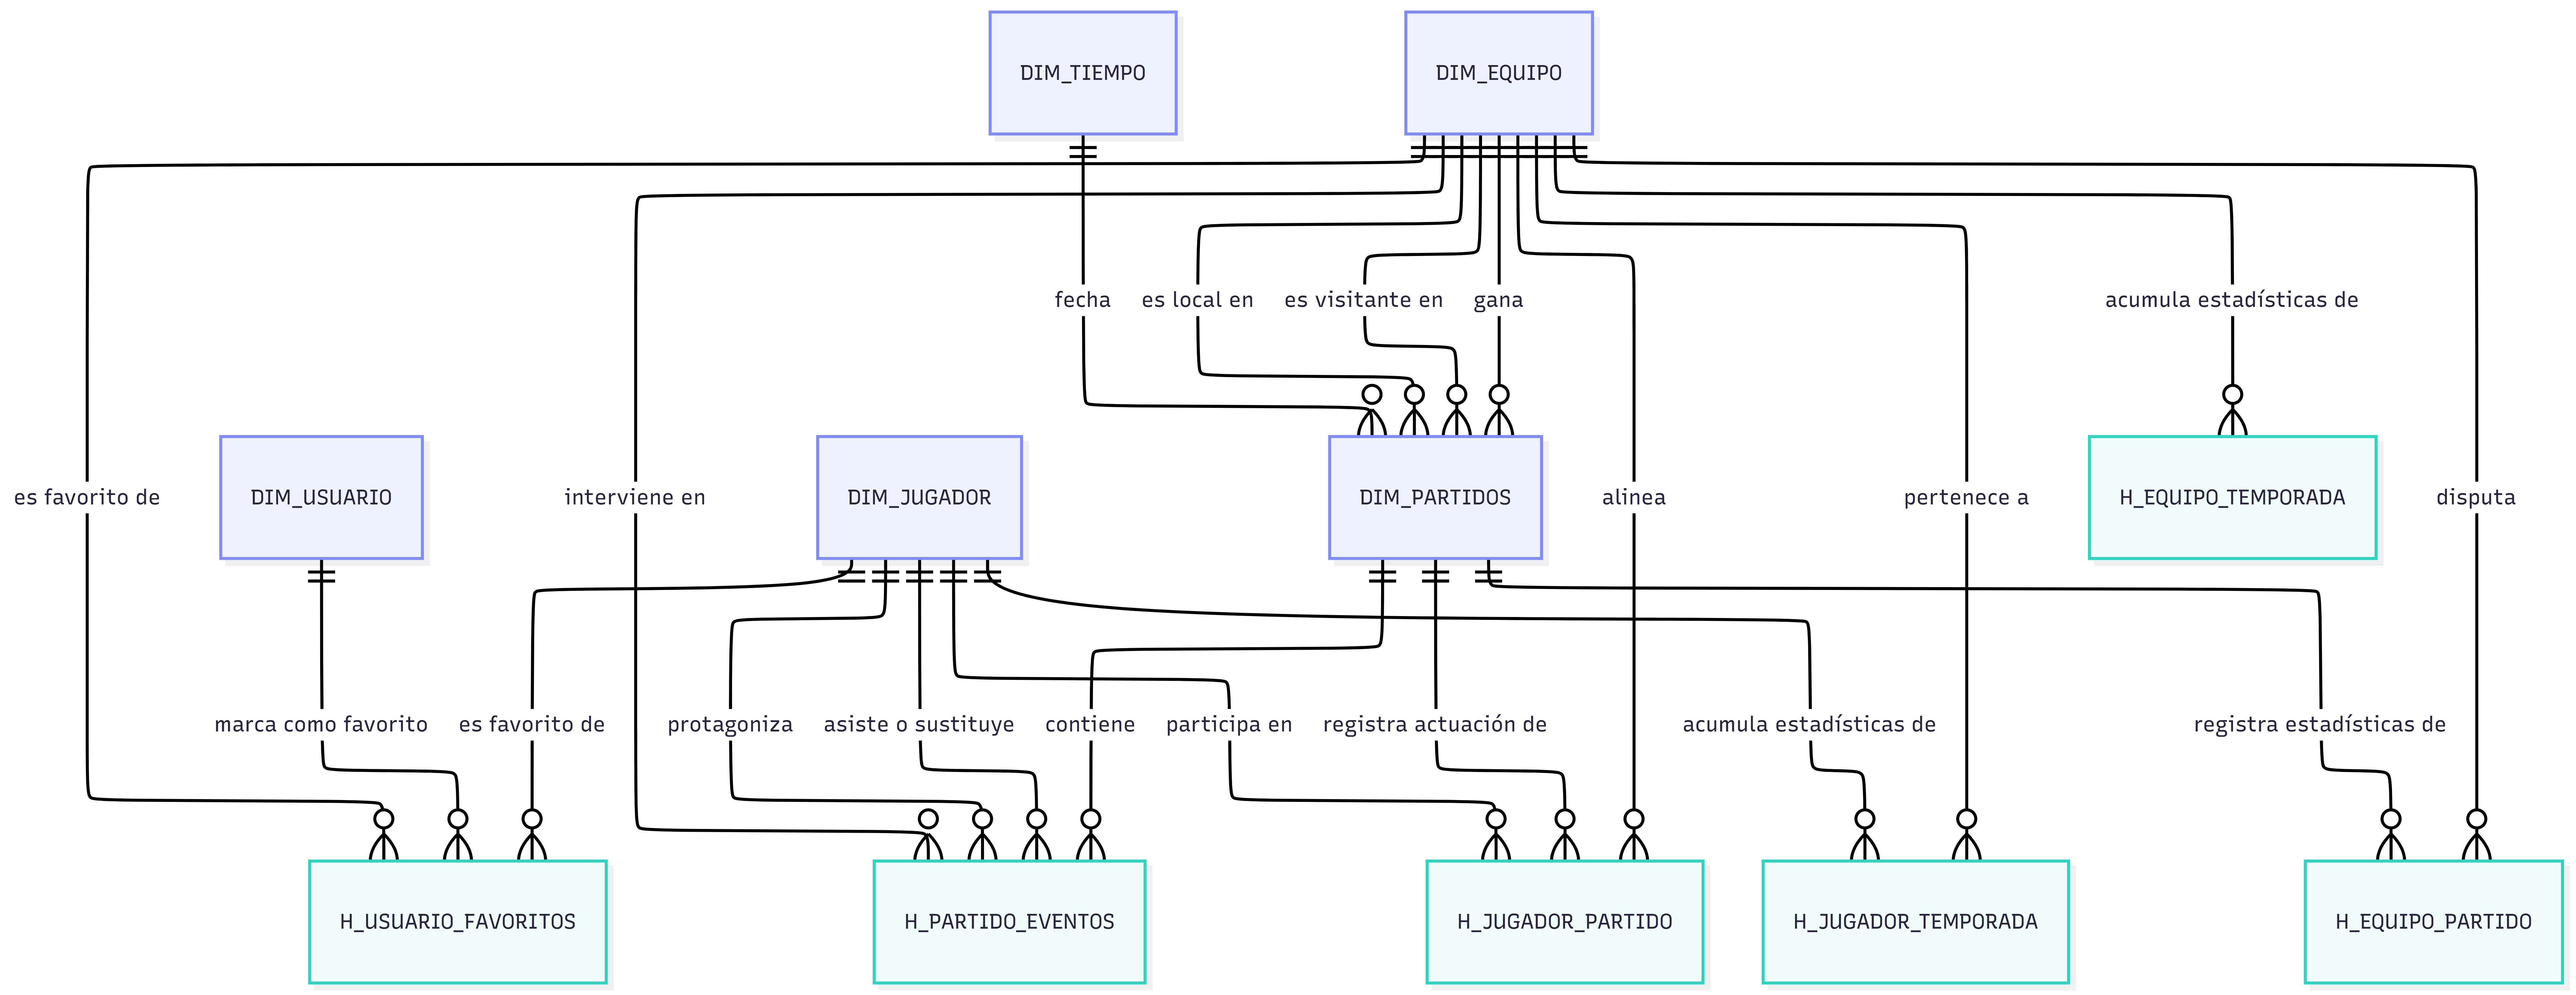
\includegraphics[width=1\linewidth]{figures/modeloER.png}
    \caption{Modelo entidad-relación del DW.}
    \label{fig:modeloER}
\end{figure}

\subsection{Modelo de casos de uso}
\subsubsection{Diagrama de caso de uso}
En este apartado se desarrollarán los casos de uso, los cuales mostrarán las acciones que los actores pueden hacer con el sistema. Específicamente, en este caso, solo tendremos un modelo de caso de uso, que será el de usuario; lo podemos ver en el diagrama de la Figura ~\ref{fig:caso de uso}, creado con la herramienta PlantUML \cite{plantuml}.
\begin{figure}[H]
    \centering
    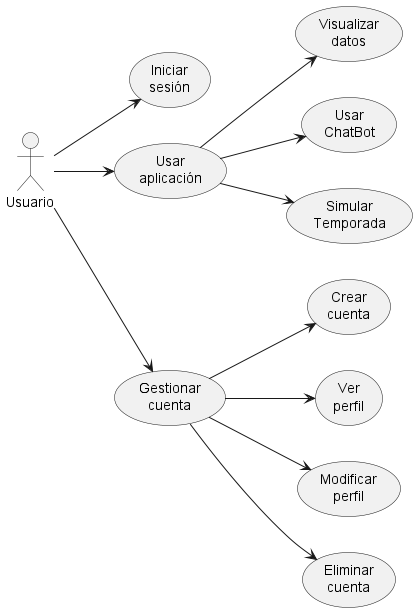
\includegraphics[width=0.6\linewidth]{figures/caso_de_uso.png}
    \caption{Modelo caso de uso: Usuario.}
    \label{fig:caso de uso}
\end{figure}

\subsubsection{Especificación de los casos de uso}

En este apartado se describen los principales casos de uso de la
aplicación. Para cada uno se indican los actores involucrados, las
precondiciones, el flujo principal, los posibles flujos alternativos
y las postcondiciones.

% ----------------------------------------------------------
\subsubsection{CU-01: Crear cuenta}

\noindent \textbf{Actor principal:} Usuario no registrado.

\noindent \textbf{Objetivo:} Crear una cuenta que permita al usuario acceder a las funcionalidades personalizadas de la aplicación.

\noindent \textbf{Precondiciones:} El usuario no ha iniciado sesión y dispone de una dirección de correo electrónico que no está registrada en el sistema.

\noindent \textbf{Disparador:} El usuario selecciona la opción \textit{Regístrate aquí}.

\noindent \textbf{Flujo principal:}
\begin{enumerate}
    \item El sistema muestra el formulario de registro.
    \item El usuario introduce su nombre de usuario, correo electrónico y contraseña.
    \item El usuario confirma la contraseña.
    \item El usuario envía el formulario.
    \item El sistema comprueba que los datos introducidos son válidos.
    \item El sistema verifica que el correo electrónico no está registrado.
    \item El sistema crea la cuenta.
    \item El sistema informa al usuario de que el registro se ha completado correctamente.
\end{enumerate}

\noindent \textbf{Flujos alternativos y excepciones:}
\begin{itemize}
    \item Si algún campo obligatorio está vacío, el sistema solicita que sea completado.
    \item Si el correo electrónico no tiene un formato válido, el sistema muestra un mensaje de error.
    \item Si el correo ya está registrado, el sistema informa al usuario y no crea la cuenta.
    \item Si las contraseñas no coinciden, el sistema solicita que se introduzcan de nuevo.
    \item Si la contraseña no cumple los requisitos de seguridad, el sistema informa de los requisitos necesarios.
\end{itemize}

\noindent \textbf{Postcondiciones:} La cuenta queda registrada y el usuario puede iniciar sesión.

\subsubsection{CU-02: Iniciar sesión}

\noindent \textbf{Actor principal:} Usuario registrado.

\noindent \textbf{Objetivo:} Autenticar al usuario para permitirle acceder a las funcionalidades restringidas de la aplicación.

\noindent \textbf{Precondiciones:} El usuario dispone de una cuenta registrada y no ha iniciado sesión.

\noindent \textbf{Disparador:} El usuario abre la aplicación.

\noindent \textbf{Flujo principal:}
\begin{enumerate}
    \item El sistema muestra el formulario de inicio de sesión.
    \item El usuario introduce su correo electrónico y contraseña.
    \item El usuario envía el formulario.
    \item El sistema valida las credenciales.
    \item El sistema inicia la sesión del usuario.
    \item El sistema redirige al usuario a la pantalla principal.
\end{enumerate}

\noindent \textbf{Flujos alternativos y excepciones:}
\begin{itemize}
    \item Si algún campo está vacío, el sistema solicita que sea completado.
    \item Si las credenciales son incorrectas, el sistema muestra un mensaje de error.
    \item Si la cuenta no existe, el sistema informa al usuario y ofrece la posibilidad de registrarse.
    \item Si ocurre un error de conexión, el sistema informa de que no ha sido posible iniciar sesión.
\end{itemize}

\noindent \textbf{Postcondiciones:} La sesión queda iniciada y el usuario puede acceder a las funcionalidades asociadas a su cuenta.

\subsubsection{CU-03: Cerrar sesión}

\noindent \textbf{Actor principal:} Usuario autenticado.

\noindent \textbf{Objetivo:} Finalizar de forma segura la sesión activa del usuario.

\noindent \textbf{Precondiciones:} El usuario ha iniciado sesión previamente.

\noindent \textbf{Disparador:} El usuario selecciona la opción \textit{Cerrar sesión}.

\noindent \textbf{Flujo principal:}
\begin{enumerate}
    \item El usuario abre el menú de su cuenta.
    \item El usuario selecciona la opción \textit{Cerrar sesión}.
    \item El sistema invalida la sesión activa.
    \item El sistema redirige al usuario a la pantalla principal o de inicio de sesión.
\end{enumerate}

\noindent \textbf{Flujos alternativos y excepciones:}
\begin{itemize}
    \item Si la sesión ya ha expirado, el sistema redirige directamente al usuario a la pantalla de inicio de sesión.
    \item Si se produce un error, el sistema elimina localmente los datos de autenticación e informa al usuario.
\end{itemize}

\noindent \textbf{Postcondiciones:} La sesión queda finalizada y las funcionalidades restringidas dejan de estar disponibles.

\subsubsection{CU-04: Visualizar datos de LaLiga}

\noindent \textbf{Actor principal:} Usuario.

\noindent \textbf{Objetivo:} Consultar la información disponible sobre LaLiga, como clasificaciones, equipos, jugadores, partidos o estadísticas.

\noindent \textbf{Precondiciones:} La aplicación está disponible y existen datos almacenados o accesibles desde la fuente de información utilizada.

\noindent \textbf{Disparador:} El usuario accede a la sección de consulta de datos.

\noindent \textbf{Flujo principal:}
\begin{enumerate}
    \item El sistema muestra las categorías de datos disponibles.
    \item El usuario selecciona una categoría.
    \item El sistema obtiene los datos correspondientes.
    \item El sistema presenta la información de forma ordenada.
    \item El usuario puede seleccionar un elemento para consultar sus detalles.
    \item El sistema muestra la información detallada del elemento seleccionado.
\end{enumerate}

\noindent \textbf{Flujos alternativos y excepciones:}
\begin{itemize}
    \item Si no existen datos para la categoría seleccionada, el sistema informa al usuario.
    \item Si la fuente externa de datos no está disponible, el sistema muestra un mensaje de error.
    \item Si el usuario realiza una búsqueda sin resultados, el sistema informa de que no se encontraron coincidencias.
    \item Si existen filtros, el usuario puede aplicarlos y el sistema actualiza la información mostrada.
\end{itemize}

\noindent \textbf{Postcondiciones:} Los datos seleccionados quedan mostrados sin modificar la información almacenada por el sistema.

\subsubsection{CU-05: Consultar al chatbot}

\noindent \textbf{Actor principal:} Usuario.

\noindent \textbf{Objetivo:} Realizar preguntas en lenguaje natural y obtener información relacionada con LaLiga.

\noindent \textbf{Precondiciones:} El chatbot está disponible y puede acceder a la información necesaria para responder.

\noindent \textbf{Disparador:} El usuario accede a la sección del chatbot.

\noindent \textbf{Flujo principal:}
\begin{enumerate}
    \item El sistema muestra la interfaz de conversación.
    \item El usuario introduce una pregunta.
    \item El sistema recibe y analiza la consulta.
    \item El sistema identifica la intención del usuario.
    \item El sistema busca o procesa la información necesaria.
    \item El chatbot genera una respuesta.
    \item El sistema muestra la respuesta en la conversación.
    \item El usuario puede realizar nuevas preguntas.
\end{enumerate}

\noindent \textbf{Flujos alternativos y excepciones:}
\begin{itemize}
    \item Si la pregunta está vacía, el sistema no la envía.
    \item Si el chatbot no comprende la consulta, solicita al usuario que la reformule.
    \item Si no existe información suficiente, el chatbot indica que no puede proporcionar una respuesta fiable.
    \item Si el servicio no está disponible, el sistema informa temporalmente de la incidencia.
\end{itemize}

\noindent \textbf{Postcondiciones:} La respuesta queda mostrada en la interfaz de conversación.

\subsubsection{CU-06: Simular una temporada}

\noindent \textbf{Actor principal:} Usuario.

\noindent \textbf{Objetivo:} Ejecutar una simulación para obtener posibles resultados y una clasificación final de la temporada.

\noindent \textbf{Precondiciones:} El sistema dispone de los datos necesarios sobre los equipos y del modelo utilizado para realizar la simulación.

\noindent \textbf{Disparador:} El usuario selecciona la opción \textit{Simular temporada}.

\noindent \textbf{Flujo principal:}
\begin{enumerate}
    \item El sistema muestra la pantalla de simulación.
    \item El sistema carga los partidos.
    \item El usuario da sus resultados de los partidos.
    \item El usuario solicita la ejecución de la simulación.
    \item El sistema valida los parámetros introducidos.
    \item El sistema ejecuta el modelo de simulación.
    \item El sistema calcula los resultados de los partidos.
    \item El sistema genera la clasificación final simulada.
    \item El sistema muestra los resultados al usuario.
\end{enumerate}

\noindent \textbf{Flujos alternativos y excepciones:}
\begin{itemize}
    \item Si los parámetros no son válidos, el sistema solicita que sean corregidos.
    \item Si faltan datos de algún equipo, el sistema informa de que la simulación no puede ejecutarse.
    \item Si ocurre un error durante el cálculo, el sistema cancela la simulación y muestra un mensaje.
    \item Si el proceso requiere tiempo adicional, el sistema muestra un indicador de progreso.
\end{itemize}

\noindent \textbf{Postcondiciones:} Los resultados y la clasificación simulada quedan disponibles para su consulta. Los datos reales de LaLiga no son modificados.

\subsubsection{CU-07: Ver perfil}

\noindent \textbf{Actor principal:} Usuario autenticado.

\noindent \textbf{Objetivo:} Consultar la información asociada a la cuenta del usuario.

\noindent \textbf{Precondiciones:} El usuario ha iniciado sesión.

\noindent \textbf{Disparador:} El usuario selecciona la opción \textit{Ver perfil}.

\noindent \textbf{Flujo principal:}
\begin{enumerate}
    \item El usuario accede al menú de su cuenta.
    \item El usuario selecciona la opción \textit{Ver perfil}.
    \item El sistema identifica al usuario autenticado.
    \item El sistema recupera la información asociada a su cuenta.
    \item El sistema muestra los datos del perfil.
\end{enumerate}

\noindent \textbf{Flujos alternativos y excepciones:}
\begin{itemize}
    \item Si la sesión ha expirado, el sistema solicita al usuario que vuelva a iniciar sesión.
    \item Si no es posible recuperar la información, el sistema muestra un mensaje de error.
\end{itemize}

\noindent \textbf{Postcondiciones:} La información del perfil queda mostrada sin realizar modificaciones.

\subsubsection{CU-08: Modificar perfil}

\noindent \textbf{Actor principal:} Usuario autenticado.

\noindent \textbf{Objetivo:} Modificar los datos personales asociados a la cuenta del usuario.

\noindent \textbf{Precondiciones:} El usuario ha iniciado sesión y su cuenta se encuentra activa.

\noindent \textbf{Disparador:} El usuario selecciona la opción \textit{Modificar perfil}.

\noindent \textbf{Flujo principal:}
\begin{enumerate}
    \item El sistema muestra los datos actuales del perfil.
    \item El usuario selecciona los datos que desea modificar.
    \item El usuario introduce los nuevos valores.
    \item El usuario confirma los cambios.
    \item El sistema valida la información introducida.
    \item El sistema actualiza el perfil.
    \item El sistema informa de que los cambios se han guardado correctamente.
\end{enumerate}

\noindent \textbf{Flujos alternativos y excepciones:}
\begin{itemize}
    \item Si un dato no tiene un formato válido, el sistema solicita que sea corregido.
    \item Si el nuevo correo ya pertenece a otra cuenta, el sistema rechaza el cambio.
    \item Si el usuario cancela la operación, el sistema mantiene los datos anteriores.
    \item Si ocurre un error durante la actualización, el sistema no guarda los cambios y muestra un mensaje.
\end{itemize}

\noindent \textbf{Postcondiciones:} Los datos válidos introducidos por el usuario quedan asociados a su cuenta.

\subsubsection{CU-09: Eliminar cuenta}

\noindent \textbf{Actor principal:} Usuario autenticado.

\noindent \textbf{Objetivo:} Eliminar la cuenta del usuario y los datos personales asociados a ella.

\noindent \textbf{Precondiciones:} El usuario ha iniciado sesión y su cuenta se encuentra activa.

\noindent \textbf{Disparador:} El usuario selecciona la opción \textit{Eliminar cuenta}.

\noindent \textbf{Flujo principal:}
\begin{enumerate}
    \item El usuario accede a la configuración de su perfil.
    \item El usuario selecciona la opción \textit{Eliminar cuenta}.
    \item El sistema advierte de las consecuencias de la operación.
    \item El sistema solicita la confirmación del usuario.
    \item El usuario confirma que desea eliminar la cuenta.
    \item El sistema verifica la identidad del usuario.
    \item El sistema elimina o anonimiza los datos asociados, según corresponda.
    \item El sistema invalida la sesión activa.
    \item El sistema informa de que la cuenta ha sido eliminada.
\end{enumerate}

\noindent \textbf{Flujos alternativos y excepciones:}
\begin{itemize}
    \item Si el usuario cancela la confirmación, el sistema no realiza ningún cambio.
    \item Si la verificación de identidad falla, el sistema cancela la operación.
    \item Si se produce un error durante la eliminación, el sistema conserva la cuenta e informa al usuario.
\end{itemize}

\noindent \textbf{Postcondiciones:} La cuenta deja de estar disponible, la sesión queda cerrada y el usuario ya no puede autenticarse con las credenciales eliminadas.

\subsection{Modelo de interfaz de usuario}
En este apartado se describe el diseño de la interfaz de usuario de la aplicación, incluyendo tanto los modelos iniciales de baja fidelidad como la organización de la navegación entre pantallas. El objetivo es definir una estructura clara, coherente y sencilla de utilizar, que facilite el acceso a la información estadística, los \textit{dashboards} y las funcionalidades avanzadas de análisis incorporadas en el sistema.

\subsubsection{Modelos de baja fidelidad}
\subsubsection{Diagrama de navegación}
La navegación de la aplicación se organiza mediante una estructura jerárquica (véase Figura~\ref{fig:navegacion}). En primer lugar, el usuario accede a través de las pantallas de autenticación, formadas por el inicio de sesión y el registro. Una vez autenticado, se muestra la aplicación principal, basada en un menú lateral desde el que se accede a las secciones principales: Inicio, Temporadas, Equipos, Jugadores, Partidos, Perfil y Ajustes.
Las secciones de consulta presentan listados o filtros iniciales que permiten acceder a pantallas de detalle. Estas pantallas utilizan pestañas superiores para organizar la información en subsecciones, evitando sobrecargar una única vista. Por ejemplo, el detalle de una temporada incluye pestañas de partidos, clasificación, rankings y análisis; el detalle de un equipo muestra información, plantilla, trayectoria y gráficos; y el detalle de un partido divide la información entre previa, alineación, eventos y post-partido.

Además, la aplicación incorpora elementos transversales como el buscador global, que permite acceder directamente a jugadores y equipos, y el asistente “Agente de Oro”, visible en las pantallas principales como punto de entrada a consultas futbolísticas.

\begin{figure}[H]
    \centering
    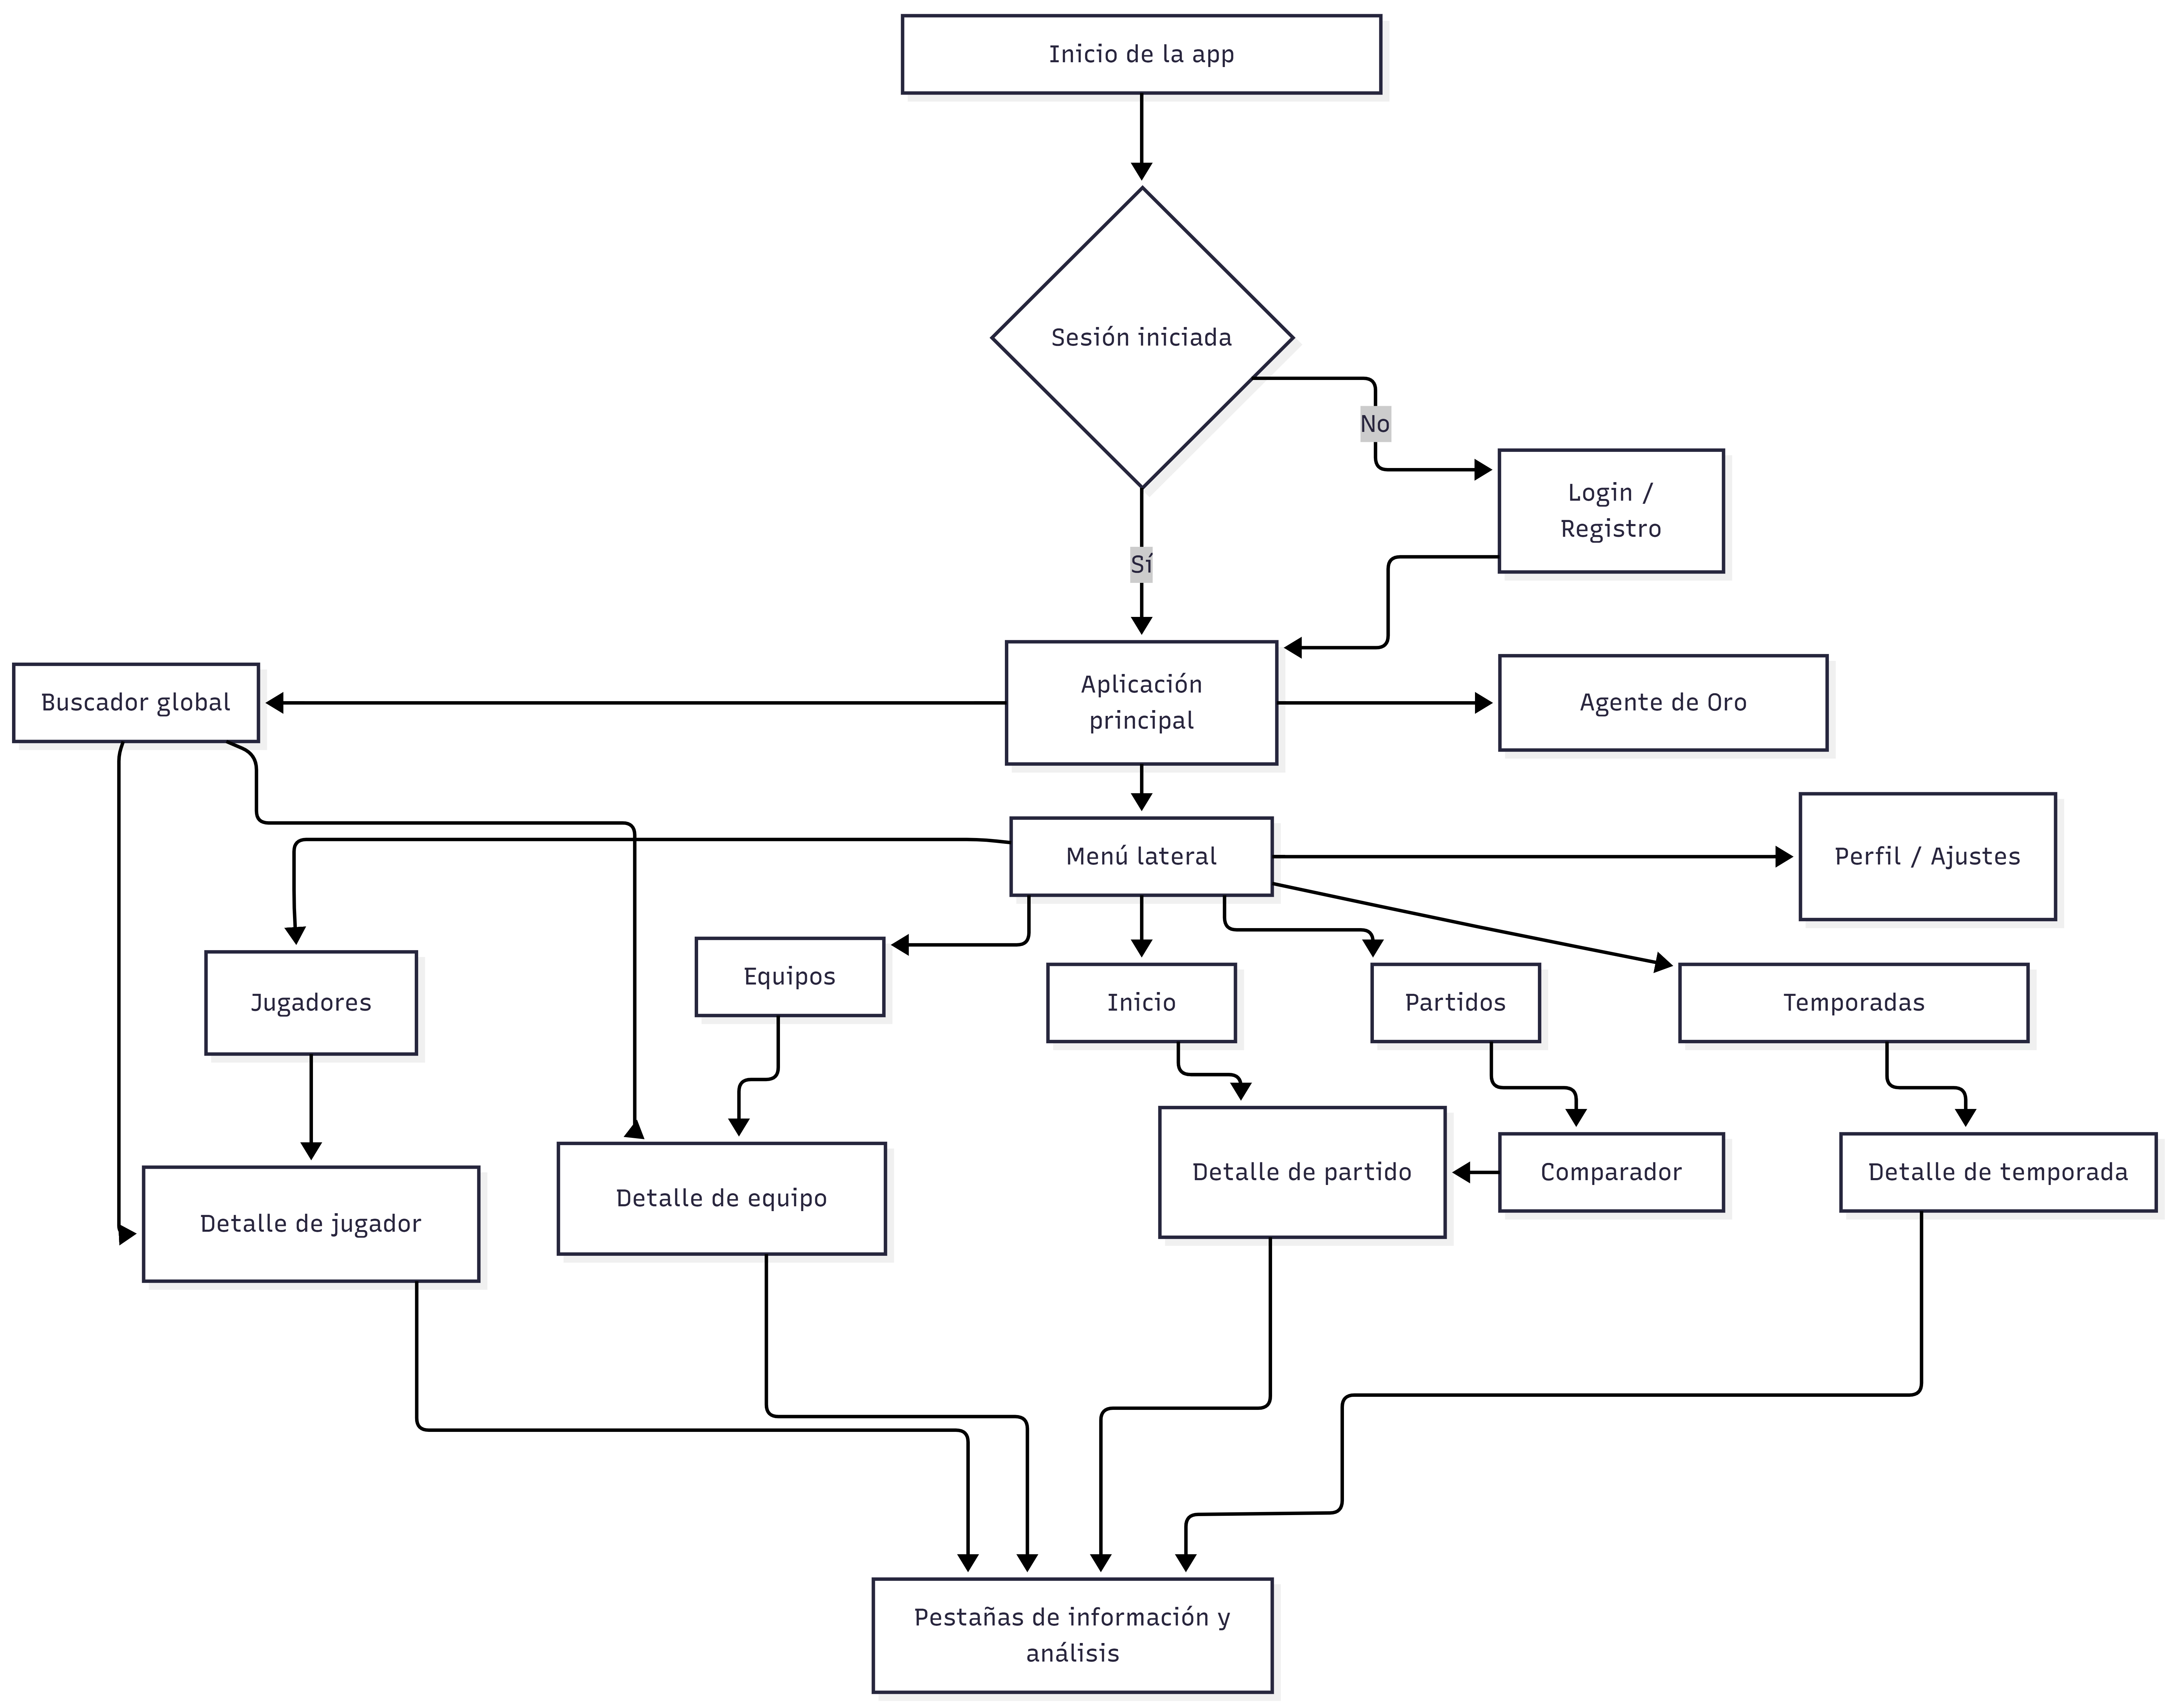
\includegraphics[width=1\linewidth]{figures/navegación.png}
    \caption{Diagrama de navegación.}
    \label{fig:navegacion}
\end{figure}
En este capítulo se recoge el diseño de la arquitectura del sistema informático, el diseño físico de datos y el diseño detallado de la interfaz de usuario.
\section{Diseño del sistema}
\subsection{Arquitectura del sistema}

La arquitectura del sistema se basa en un modelo de flujo de datos enriquecido, donde la información es captada, procesada y transformada mediante técnicas de analítica avanzada antes de su almacenamiento y exposición. El diseño estructural, representado en la Figura \ref{fig:arquitectura}, se divide en las siguientes etapas funcionales:

\begin{figure}[H]
    \centering
    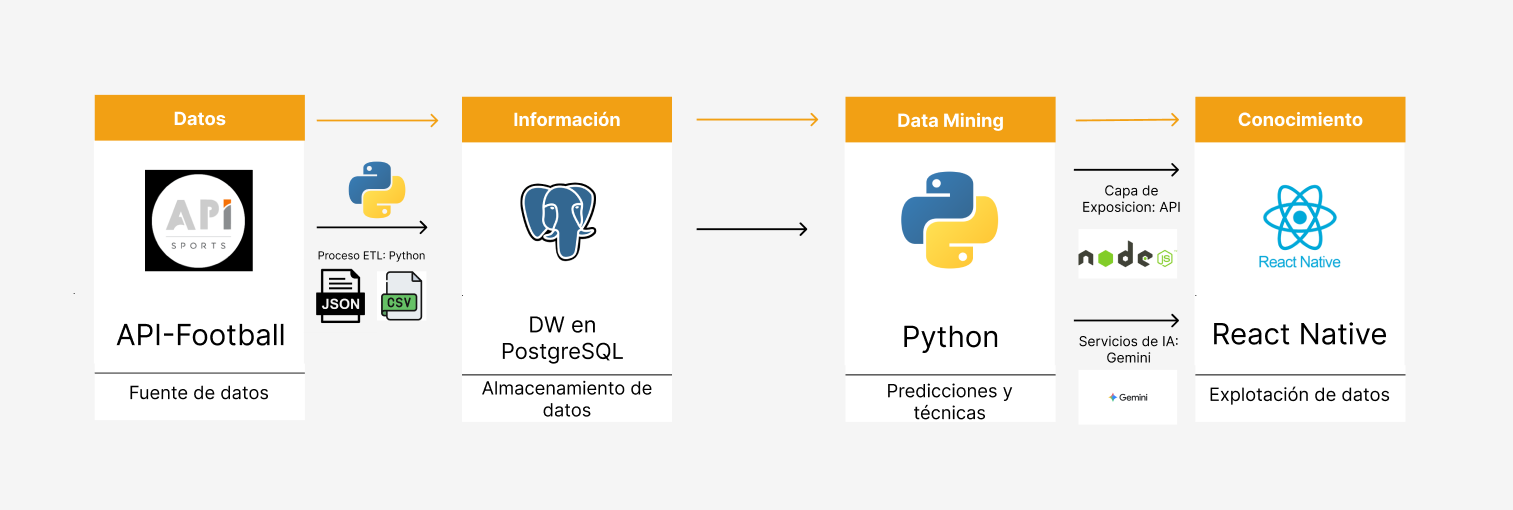
\includegraphics[width=1\linewidth]{figures/arquitectura_bi.png}
    \caption{Arquitectura BI.}
    \label{fig:arquitectura}
\end{figure}

\begin{itemize}
    \item Fuentes de datos (Ingesta): punto de entrada encargado de la extracción de información en bruto desde la API externa API-FOOTBALL en formato JSON.
    \item Proceso ETL: capa de procesamiento desarrollada en Python mediante las librerías pandas y numpy para la limpieza y transformación de archivos JSON a estructuras tabulares CSV.
    \item \textit{Data mining}: motor de analítica avanzada basado en scikit-learn donde se ejecutan los modelos de aprendizaje automático para la generación de métricas predictivas y los algoritmos de métricas estadísticas.
    \item Capa de información: almacén de datos centralizado en PostgreSQL, gestionado mediante DBeaver, que garantiza la persistencia e integridad de los datos procesados.
    \item Capa de exposicion (API): interfaz de servicios desarrollada en Node.js y
    Express, que actúa como puente de comunicación entre PostgreSQL, los servicios
    analíticos, el chatbot y el cliente móvil, y consulta entre el almacén de datos y el cliente.
    \item Servicios de IA: dentro de la capa backend se integran servicios avanzados como la API de Gemini, como el chatbot basado en IA generativa, que permite consultar la base de datos mediante preguntas en lenguaje natural, y el módulo de simulación, que ejecuta escenarios personalizados a partir de los resultados introducidos por el usuario.
    \item Explotación de datos: capa de presentación final desarrollada en React Native, encargada de la visualización de la información y los resultados del análisis para el usuario.
\end{itemize}

\subsection{Diseño físico de datos}

En esta sección se define la estructura física de datos que utilizará el sistema, a partir del modelo conceptual de clases, de manera que, teniendo presentes los requisitos establecidos para el sistema de información y las particularidades del entorno tecnológico, se consiga un acceso eficiente a los datos. La estructura física se compone de tablas, índices, procedimientos almacenados, secuencias y otros elementos dependientes del SGBD utilizado.

El diseño físico de la base de datos se ha planteado siguiendo un esquema en constelación, propio de entornos de \textit{data warehouse}. Este tipo de modelo se caracteriza por la existencia de varias tablas de hechos que comparten dimensiones comunes, permitiendo analizar la información desde distintas perspectivas. En el caso de este proyecto, las tablas de hechos almacenan métricas relacionadas con partidos, jugadores, equipos, temporadas y eventos, mientras que las tablas de dimensiones contienen información descriptiva como equipos, jugadores, partidos o tiempo. Esta organización facilita la realización de consultas analíticas, la generación de indicadores y la explotación posterior de los datos mediante técnicas de \textit{business intelligence} y \textit{data mining}.

Dentro de este modelo, las tablas de dimensiones representan entidades descriptivas del sistema y permiten contextualizar los datos almacenados. Por ejemplo, una dimensión puede contener información sobre un equipo, un jugador, un partido o una temporada. Por otro lado, las tablas de hechos almacenan datos cuantitativos o medibles, normalmente asociados a una o varias dimensiones. En este proyecto, estas tablas recogen estadísticas de rendimiento, resultados, eventos y métricas acumuladas, permitiendo analizar el comportamiento deportivo desde diferentes niveles de detalle.

\begin{figure}[H]
    \centering
    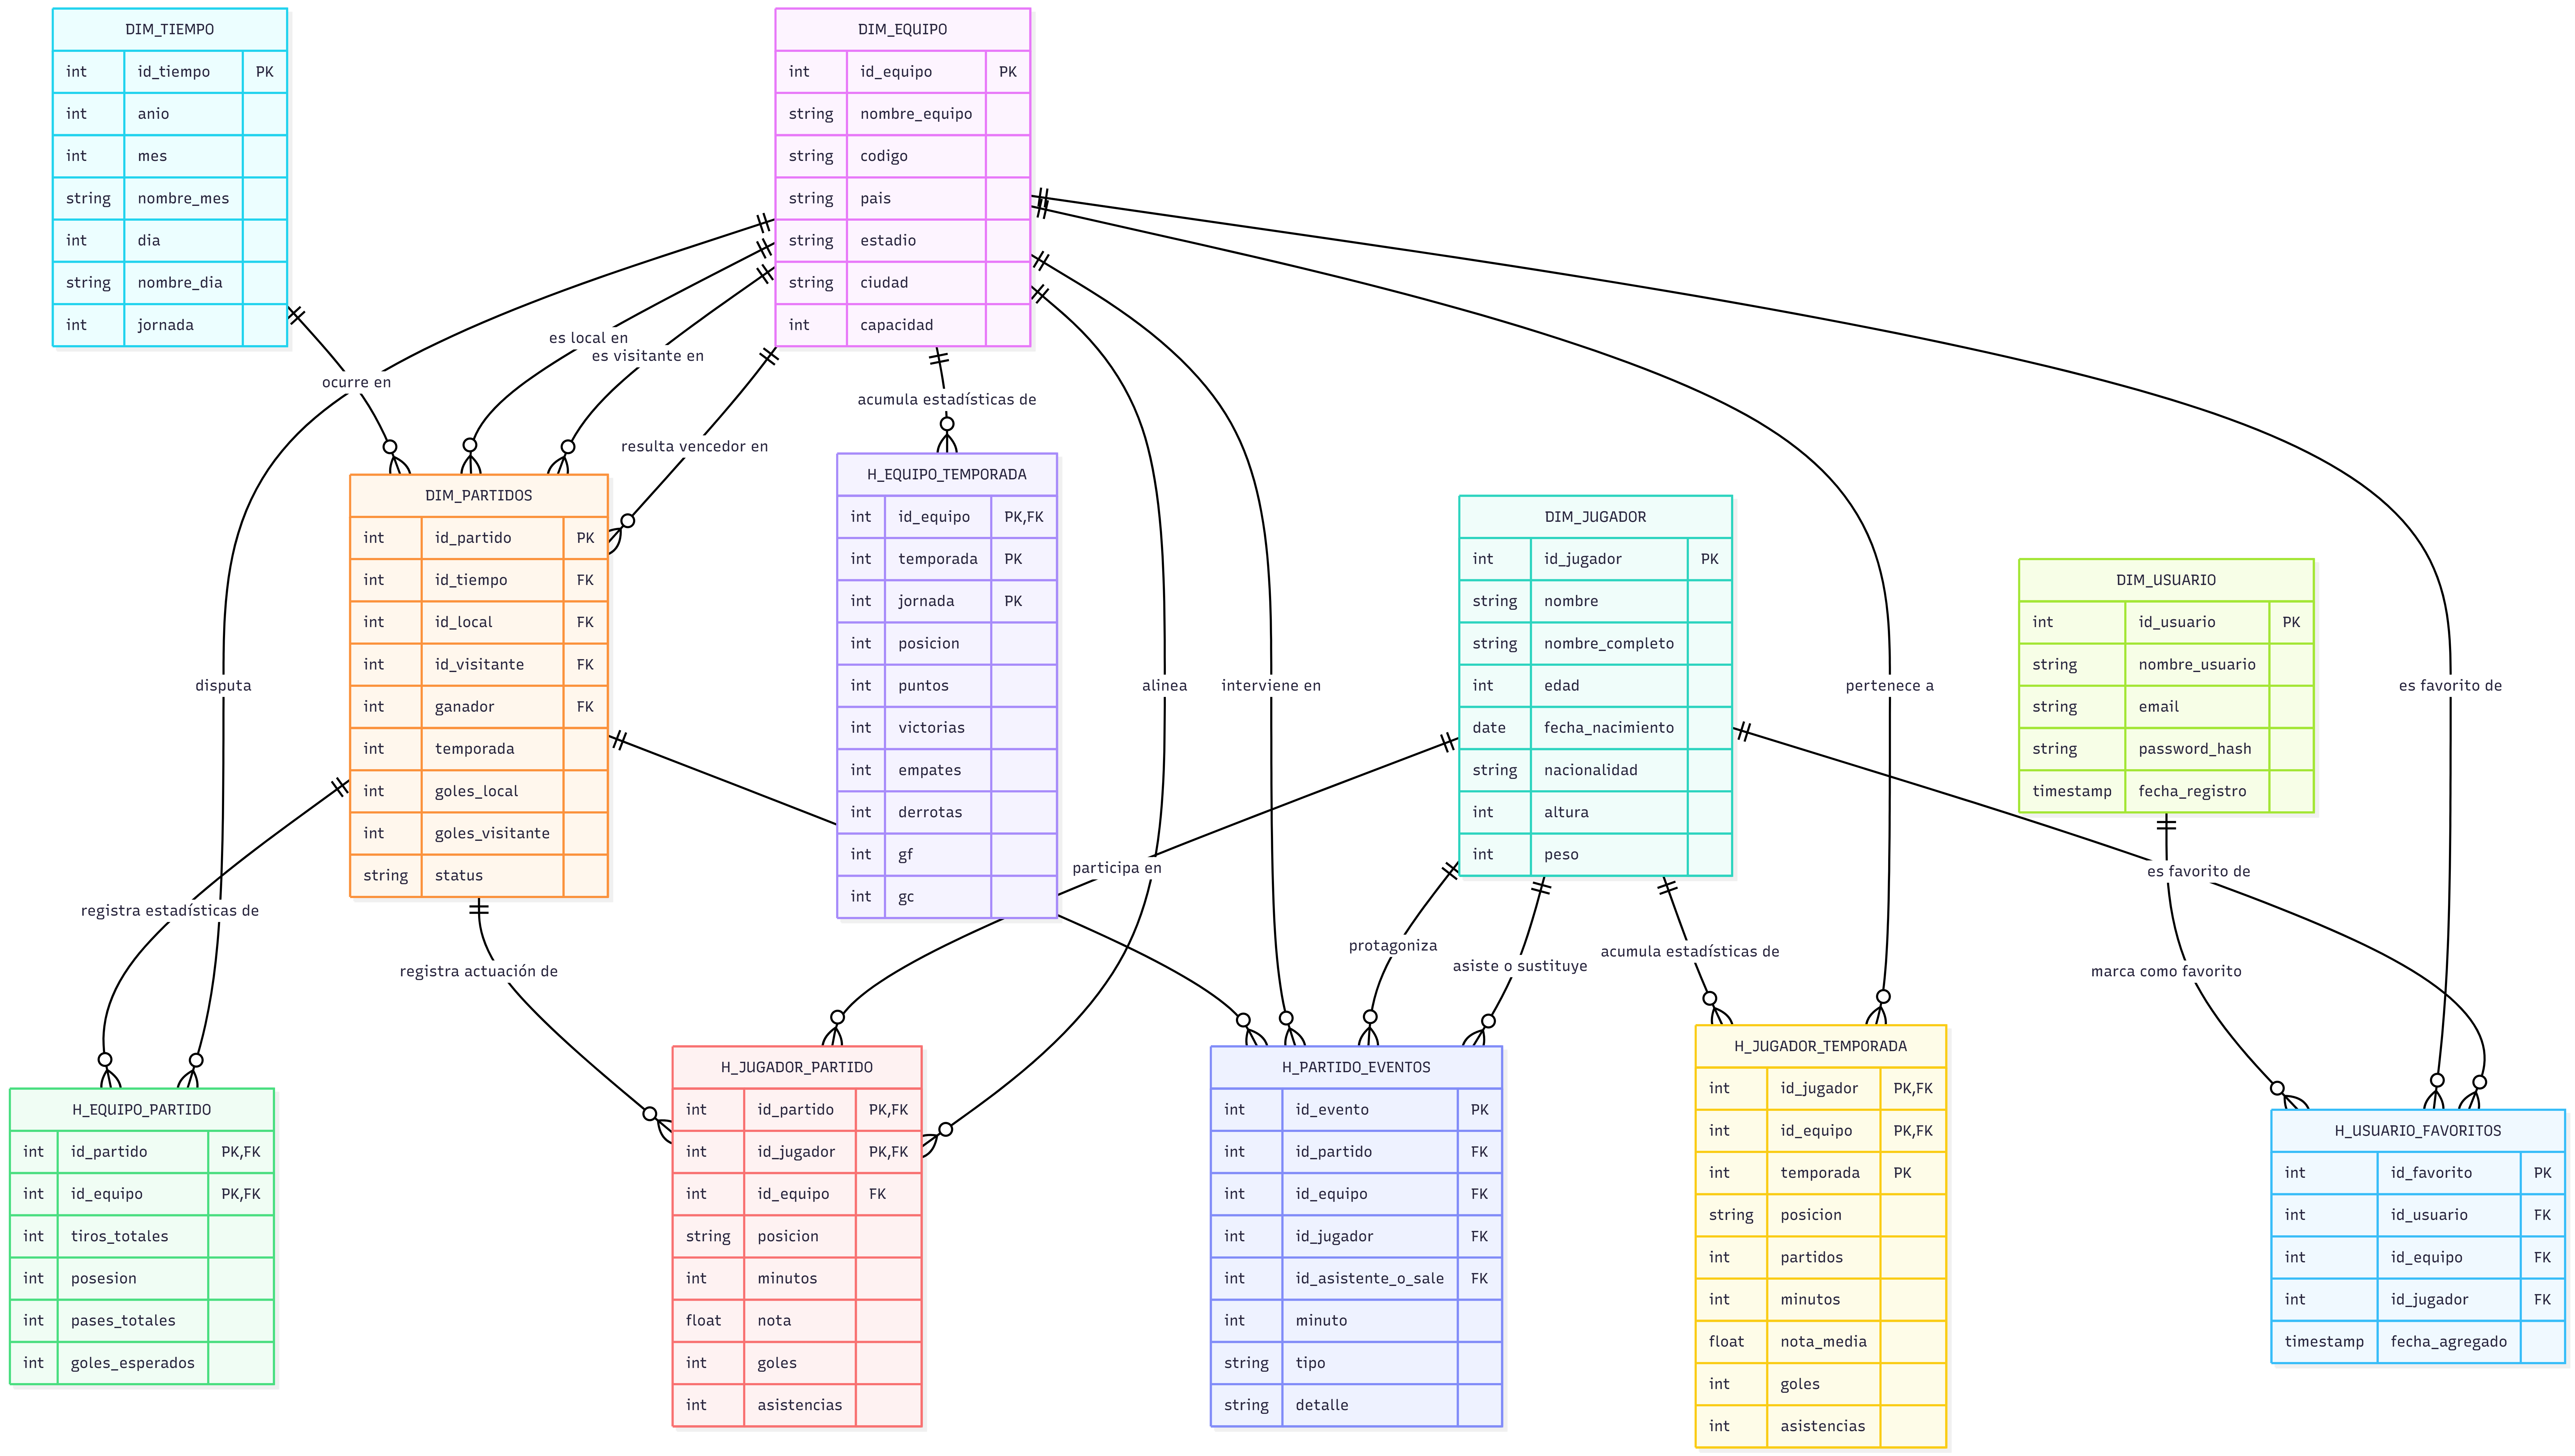
\includegraphics[width=1\linewidth]{figures/modelo_fisico.png}
    \caption{Modelo físico de la base de datos.}
    \label{fig:modelo_fisico}
\end{figure}

A continuación se describen las principales tablas que componen el modelo físico de datos. Para cada una de ellas se indican sus atributos más relevantes y su función dentro del sistema.
\subsubsection{Tablas de dimensión}

\begin{longtable}{|l|l|}
\caption{Atributos de la tabla dim\_equipo.} \\

\hline
\textbf{Atributo} & \textbf{Descripción} \\
\hline
\endfirsthead

\hline
\textbf{Atributo} & \textbf{Descripción} \\
\hline
\endhead

\hline
\multicolumn{2}{r}{\textit{Continúa en la siguiente página}} \\
\hline
\endfoot

\hline
\endlastfoot

id\_equipo & Identificador único del equipo. \\
nombre\_equipo & Nombre del equipo. \\
codigo & Código abreviado del equipo. \\
pais & País del equipo. \\
fundado\_en & Año de fundación.\\
logo & URL o ruta del escudo.\\
estadio & Nombre del estadio.\\
direccion & Dirección del estadio. \\
ciudad & Ciudad del equipo. \\
capacidad & Capacidad del estadio. \\
\hline

\end{longtable}

\begin{longtable}{|l|l|}
\caption{Atributos de la tabla dim\_jugador.} \\

\hline
\textbf{Atributo} & \textbf{Descripción} \\
\hline
\endfirsthead

\hline
\textbf{Atributo} & \textbf{Descripción} \\
\hline
\endhead

\hline
\multicolumn{2}{r}{\textit{Continúa en la siguiente página}} \\
\hline
\endfoot

\hline
\endlastfoot

id\_jugador & Identificador único del jugador. \\
nombre & Nombre deportivo del jugador. \\
nombre\_completo & Nombre completo del jugador. \\
edad & Edad del jugador. \\
fecha\_nacimiento & Fecha de nacimiento. \\
lugar\_nacimiento & Lugar de nacimiento. \\
pais\_nacimiento & País de nacimiento. \\
nacionalidad & Nacionalidad del jugador. \\
altura & Altura en centímetros. \\
peso & Peso en kilogramos. \\
foto & URL o ruta de la imagen del jugador. \\
\hline

\end{longtable}

\begin{longtable}{|l|l|}
\caption{Atributos de la tabla dim\_partidos.} \\

\hline
\textbf{Atributo} & \textbf{Descripción} \\
\hline
\endfirsthead

\hline
\textbf{Atributo} & \textbf{Descripción} \\
\hline
\endhead

\hline
\multicolumn{2}{r}{\textit{Continúa en la siguiente página}} \\
\hline
\endfoot

\hline
\endlastfoot

id\_partido & Identificador único del partido. \\
id\_tiempo & Referencia temporal del partido. \\
hora & Hora de disputa. \\
arbitro & Árbitro del encuentro. \\
estadio & Estadio del partido. \\
temporada & Temporada a la que pertenece. \\
id\_local & Equipo local. \\
id\_visitante & Equipo visitante. \\
ganador & Equipo ganador del partido. \\
goles\_local & Goles anotados por el local. \\
goles\_visitante & Goles anotados por el visitante. \\
status & Estado del partido. \\
\hline

\end{longtable}

\begin{longtable}{|l|l|}
\caption{Atributos de la tabla dim\_tiempo.} \\

\hline
\textbf{Atributo} & \textbf{Descripción} \\
\hline
\endfirsthead

\hline
\textbf{Atributo} & \textbf{Descripción} \\
\hline
\endhead

\hline
\multicolumn{2}{r}{\textit{Continúa en la siguiente página}} \\
\hline
\endfoot

\hline
\endlastfoot

id\_tiempo & Identificador temporal. \\
anio & Año. \\
mes & Número del mes. \\
nombre\_mes & Nombre del mes. \\
dia & Día del mes. \\
nombre\_dia & Nombre del día de la semana. \\
jornada & Jornada de la competición. \\
\hline

\end{longtable}

\subsubsection{Tablas de hechos}

\begin{longtable}{|l|l|}
\caption{Atributos de la tabla h\_equipo\_partido.} \\

\hline
\textbf{Atributo} & \textbf{Descripción} \\
\hline
\endfirsthead

\hline
\textbf{Atributo} & \textbf{Descripción} \\
\hline
\endhead

\hline
\multicolumn{2}{r}{\textit{Continúa en la siguiente página}} \\
\hline
\endfoot

\hline
\endlastfoot

id\_partido & Partido al que pertenecen las estadísticas. \\
id\_equipo & Equipo analizado. \\
tiros\_a\_puerta & Tiros realizados a portería. \\
tiros\_totales & Total de tiros. \\
tiros\_en\_area & Tiros realizados dentro del área. \\
tiros\_fuera\_area & Tiros realizados fuera del área. \\
faltas\_cometidas & Faltas realizadas. \\
corners & Saques de esquina. \\
fueras\_de\_juego & Fueras de juego. \\
posesion & Porcentaje de posesión. \\
tarjetas\_amarillas & Tarjetas amarillas recibidas. \\
tarjetas\_rojas & Tarjetas rojas recibidas. \\
paradas & Paradas realizadas. \\
pases\_totales & Total de pases. \\
pases\_acertados & Pases completados. \\
pct\_pases\_acertados & Porcentaje de acierto en pases. \\
goles\_esperados & Valor de goles esperados. \\
df\_goles\_esperados & Diferencia respecto a goles esperados. \\
\hline

\end{longtable}

\begin{longtable}{|l|l|}
\caption{Atributos de la tabla h\_equipo\_temporada.} \\

\hline
\textbf{Atributo} & \textbf{Descripción} \\
\hline
\endfirsthead

\hline
\textbf{Atributo} & \textbf{Descripción} \\
\hline
\endhead

\hline
\multicolumn{2}{r}{\textit{Continúa en la siguiente página}} \\
\hline
\endfoot

\hline
\endlastfoot

id\_equipo & Equipo al que pertenece el registro. \\
temporada & Temporada analizada. \\
jornada & Jornada correspondiente. \\
posicion & Posición en la clasificación. \\
nombre\_equipo & Nombre del equipo. \\
puntos & Puntos acumulados. \\
dg & Diferencia de goles. \\
forma & Racha reciente del equipo. \\
partidos\_jugados & Partidos disputados. \\
victorias & Victorias totales. \\
empates & Empates totales. \\
derrotas & Derrotas totales. \\
gf & Goles a favor. \\
gc & Goles en contra. \\
victorias\_local & Victorias como local. \\
empates\_local & Empates como local. \\
derrotas\_local & Derrotas como local. \\
victorias\_visitante & Victorias como visitante. \\
empates\_visitante & Empates como visitante. \\
derrotas\_visitante & Derrotas como visitante. \\
\hline

\end{longtable}

\begin{longtable}{|l|l|}
\caption{Atributos de la tabla h\_jugador\_partido.} \\

\hline
\textbf{Atributo} & \textbf{Descripción} \\
\hline
\endfirsthead

\hline
\textbf{Atributo} & \textbf{Descripción} \\
\hline
\endhead

\hline
\multicolumn{2}{r}{\textit{Continúa en la siguiente página}} \\
\hline
\endfoot

\hline
\endlastfoot

id\_partido & Partido disputado. \\
id\_jugador & Jugador analizado. \\
id\_equipo & Equipo del jugador. \\
posicion & Posición ocupada en el partido. \\
minutos & Minutos disputados. \\
nota & Valoración del jugador. \\
capitan & Indica si fue capitán. \\
sustituto & Indica si fue suplente. \\
goles & Goles anotados. \\
asistencias & Asistencias realizadas. \\
paradas & Paradas realizadas. \\
goles\_concedidos & Goles concedidos. \\
tiros\_totales & Tiros totales. \\
tiros\_a\_puerta & Tiros a puerta. \\
pases\_totales & Pases realizados. \\
pases\_clave & Pases clave. \\
precision\_pases & Precisión de pase. \\
regates & Regates completados. \\
duelos\_totales & Duelos disputados. \\
duelos\_ganados & Duelos ganados. \\
faltas\_cometidas & Faltas realizadas. \\
faltas\_recibidas & Faltas recibidas. \\
entradas & Entradas realizadas. \\
bloqueos & Bloqueos realizados. \\
intercepciones & Intercepciones realizadas. \\
amarilla & Tarjetas amarillas. \\
roja & Tarjetas rojas. \\
\hline

\end{longtable}

\begin{longtable}{|l|l|}
\caption{Atributos de la tabla h\_jugador\_temporada.} \\

\hline
\textbf{Atributo} & \textbf{Descripción} \\
\hline
\endfirsthead

\hline
\textbf{Atributo} & \textbf{Descripción} \\
\hline
\endhead

\hline
\multicolumn{2}{r}{\textit{Continúa en la siguiente página}} \\
\hline
\endfoot

\hline
\endlastfoot

id\_jugador & Jugador analizado. \\
id\_equipo & Equipo del jugador. \\
temporada & Temporada correspondiente. \\
posicion & Posición habitual del jugador. \\
partidos & Partidos disputados. \\
minutos & Minutos jugados. \\
titular & Partidos como titular. \\
nota\_media & Valoración media. \\
goles & Goles anotados. \\
asistencias & Asistencias realizadas. \\
tiros\_totales & Tiros totales. \\
tiros\_a\_puerta & Tiros a puerta. \\
pases\_totales & Pases realizados. \\
pases\_clave & Pases clave. \\
precision\_pases & Precisión de pase. \\
entradas & Entradas realizadas. \\
bloqueos & Bloqueos realizados. \\
intercepciones & Intercepciones realizadas. \\
duelos\_totales & Duelos disputados. \\
duelos\_ganados & Duelos ganados. \\
faltas\_sufridas & Faltas recibidas. \\
faltas\_cometidas & Faltas realizadas. \\
regates\_intentados & Regates intentados. \\
regates\_exito & Regates completados. \\
amarillas & Tarjetas amarillas. \\
rojas & Tarjetas rojas. \\
goles\_concedidos & Goles concedidos. \\
paradas & Paradas realizadas. \\
\hline

\end{longtable}

\begin{longtable}{|l|l|}
\caption{Atributos de la tabla h\_partido\_eventos.} \\

\hline
\textbf{Atributo} & \textbf{Descripción} \\
\hline
\endfirsthead

\hline
\textbf{Atributo} & \textbf{Descripción} \\
\hline
\endhead

\hline
\multicolumn{2}{r}{\textit{Continúa en la siguiente página}} \\
\hline
\endfoot

\hline
\endlastfoot

id\_evento & Identificador único del evento. \\
id\_partido & Partido en el que ocurre el evento. \\
minuto & Minuto del evento. \\
extra & Tiempo añadido. \\
id\_equipo & Equipo relacionado con el evento. \\
id\_jugador & Jugador protagonista del evento. \\
id\_asistente\_o\_sale & Jugador asistente o sustituido. \\
tipo & Tipo de evento. \\
detalle & Detalle del evento. \\
comentarios & Comentarios adicionales. \\
\hline

\end{longtable}

\subsubsection{Tablas de usuario}

\begin{longtable}{|l|l|}
\caption{Atributos de la tabla dim\_usuario.} \\

\hline
\textbf{Atributo} & \textbf{Descripción} \\
\hline
\endfirsthead

\hline
\textbf{Atributo} & \textbf{Descripción} \\
\hline
\endhead

\hline
\multicolumn{2}{r}{\textit{Continúa en la siguiente página}} \\
\hline
\endfoot

\hline
\endlastfoot

id\_usuario & Identificador único del usuario. \\
nombre\_usuario & Nombre de usuario. \\
email & Correo electrónico del usuario. \\
password\_hash & Contraseña cifrada. \\
fecha\_registro & Fecha de registro en el sistema. \\
\hline

\end{longtable}

\begin{longtable}{|l|l|}
\caption{Atributos de la tabla h\_usuario\_favoritos.} \\

\hline
\textbf{Atributo} & \textbf{Descripción} \\
\hline
\endfirsthead

\hline
\textbf{Atributo} & \textbf{Descripción} \\
\hline
\endhead

\hline
\multicolumn{2}{r}{\textit{Continúa en la siguiente página}} \\
\hline
\endfoot

\hline
\endlastfoot

id\_favorito & Identificador único del favorito. \\
id\_usuario & Usuario que guarda el favorito. \\
id\_equipo & Equipo marcado como favorito. \\
id\_jugador & Jugador marcado como favorito. \\
fecha\_agregado & Fecha en la que se añadió el favorito. \\
\hline

\end{longtable}

\subsection{Diseño de tablas de \textit{data mining}}

Los algoritmos de minería de datos desarrollados en este trabajo generan una serie de tablas auxiliares que almacenan los resultados obtenidos por cada técnica de análisis. Estas tablas no forman parte del modelo conceptual principal del sistema, sino que constituyen una capa analítica utilizada por la aplicación para mostrar predicciones, simulaciones e indicadores avanzados.

Cada tabla es generada automáticamente mediante scripts desarrollados en Python, cuyos resultados son posteriormente almacenados en la base de datos PostgreSQL para ser consumidos por la API y la aplicación móvil.

\renewcommand{\arraystretch}{1.2}
\begin{longtable}{|p{4cm}|p{3cm}|p{2.2cm}|p{5cm}|}
\caption{Diseño de las tablas de \textit{data mining} implementadas.}
\label{tab:tablas_dm} \\

\hline
\textbf{Tabla} & \textbf{Algoritmo} & \textbf{Clave primaria} & \textbf{Descripción} \\
\hline
\endfirsthead

\hline
\textbf{Tabla} & \textbf{Algoritmo} & \textbf{Clave primaria} & \textbf{Descripción} \\
\hline
\endhead

\hline
\multicolumn{4}{r}{\textit{Continúa en la siguiente página}} \\
\hline
\endfoot

\hline
\endlastfoot

\path{dm_estado_forma_jugadores} &
Índice de forma &
\texttt{id\_jugador} &
Almacena el estado de forma actual de cada jugador y su evolución reciente. \\
\hline

\path{dm_estado_forma_equipos} &
Índice de forma &
\texttt{id\_equipo} &
Almacena el estado de forma actual de cada equipo junto con indicadores de tendencia y variabilidad. \\
\hline

\path{dm_perfil_estadistico_jugadores} &
Métricas estadísticas &
\texttt{id\_jugador, temporada} &
Contiene el perfil estadístico de cada jugador en distintas dimensiones del juego. \\
\hline

\path{dm_necesidades_plantilla} &
Reglas heurísticas &
\texttt{id\_equipo, temporada, necesidad} &
Recoge las necesidades detectadas en la plantilla de cada equipo y la causa que las justifica. \\
\hline

\path{dm_recomendacion_fichajes} &
Reglas heurísticas &
\texttt{id\_equipo, id\_jugador, necesidad} &
Acosia las necesidades de cada equipo en la temporada actual con jugadores que encajen con lo que buscan, generando una recomendación por necesidad. \\
\hline

\path{dm_probables_goleadores} &
Cálculo heurístico &
\texttt{id\_partido, id\_jugador} &
Contiene los jugadores con mayor probabilidad de marcar en cada partido. \\
\hline

\path{dm_prediccion_partidos} &
SVM &
\texttt{id\_partido} &
Almacena las probabilidades de victoria local, empate y victoria visitante para cada partido pendiente. \\
\hline

\path{dm_simulacion_montecarlo} &
Monte Carlo &
\texttt{id\_equipo} &
Guarda las probabilidades de campeón, clasificación europea, permanencia y descenso de cada equipo. \\
\hline

\path{dm_similitud_jugadores} &
K-means &
\texttt{id\_jugador, temporada} &
Agrupa a los jugadores según la similitud de sus características estadísticas e identifica los cinco jugadores más parecidos. \\
\hline

\path{dm_golesesperados_partidos} &
Random Forest Regressor &
\texttt{id\_partido} &
Almacena el número estimado de goles que marcará cada equipo en un partido. \\
\hline

\end{longtable}
\subsection{Diseño de la interfaz de usuario} 
En esta sección se presenta el diseño visual final de la aplicación, describiendo la organización de las pantallas, la distribución de los elementos de la interfaz y las decisiones tomadas en relación con la identidad visual del sistema. Además, se detallan aspectos como el logotipo, la paleta de colores y el nombre de la aplicación, con el objetivo de mostrar cómo se ha construido una interfaz coherente, intuitiva y adaptada al contexto de una aplicación de análisis futbolístico.
\subsection{Diseño final}

El diseño final de la aplicación mantiene la idea inicial de ofrecer una herramienta visual e intuitiva para consultar información relacionada con LaLiga, aunque durante el desarrollo se incorporaron nuevas funcionalidades que hicieron necesario adaptar varias pantallas. En la versión final no solo se permite consultar equipos, jugadores, partidos y temporadas, sino también acceder a análisis estadísticos, simulaciones, predicciones y consultas mediante inteligencia artificial.

La interfaz se ha organizado para facilitar la navegación entre las distintas secciones principales de la aplicación. Para ello se utilizaron vistas diferenciadas para el acceso de usuarios, la consulta de información deportiva, las funcionalidades avanzadas y la configuración. Además, se incorporó soporte para tema claro y tema oscuro.

La navegación principal se realiza mediante un menú desde el que el usuario puede acceder a las diferentes funcionalidades, junto con un buscador que facilita la localización de información dentro del sistema.

\begin{figure}[H]
\centering
\begin{subfigure}[b]{0.4\textwidth}
\centering
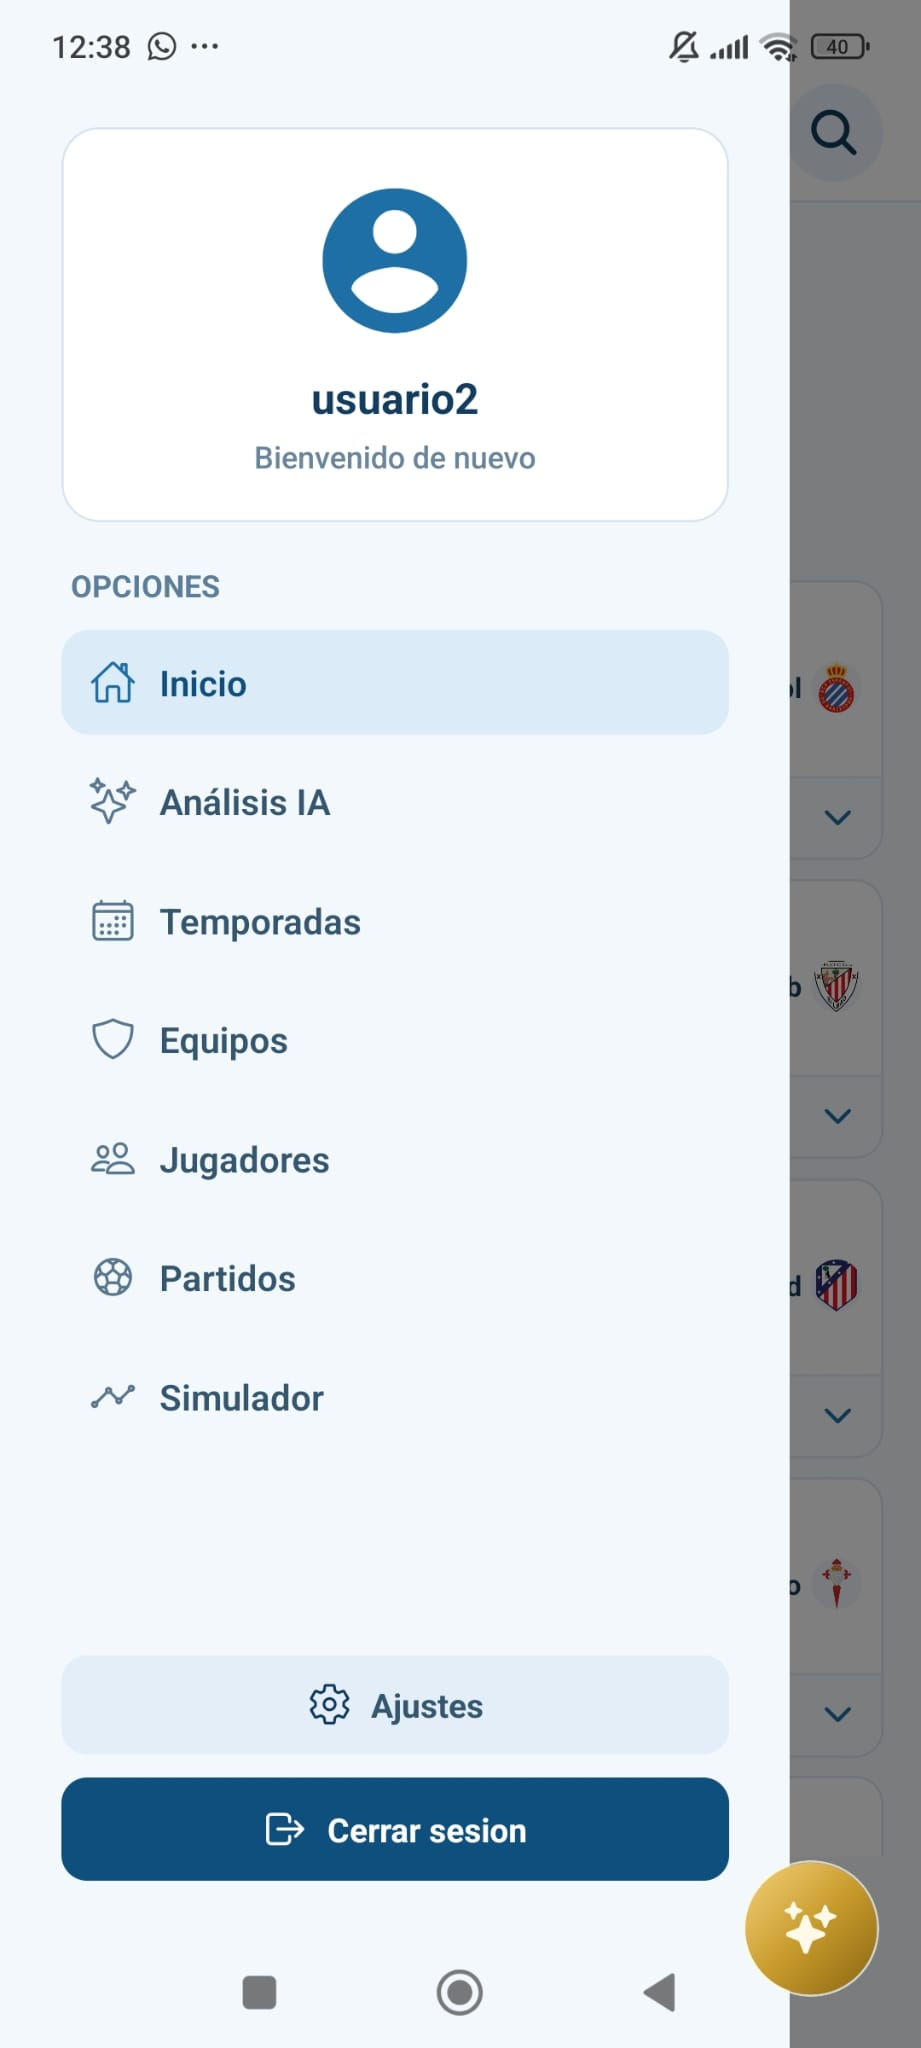
\includegraphics[width=0.5\textwidth]{figures/cap_menu.jpeg}
\caption{Menú principal}
\label{fig:menu}
\end{subfigure}
%
\begin{subfigure}[b]{0.4\textwidth}
\centering
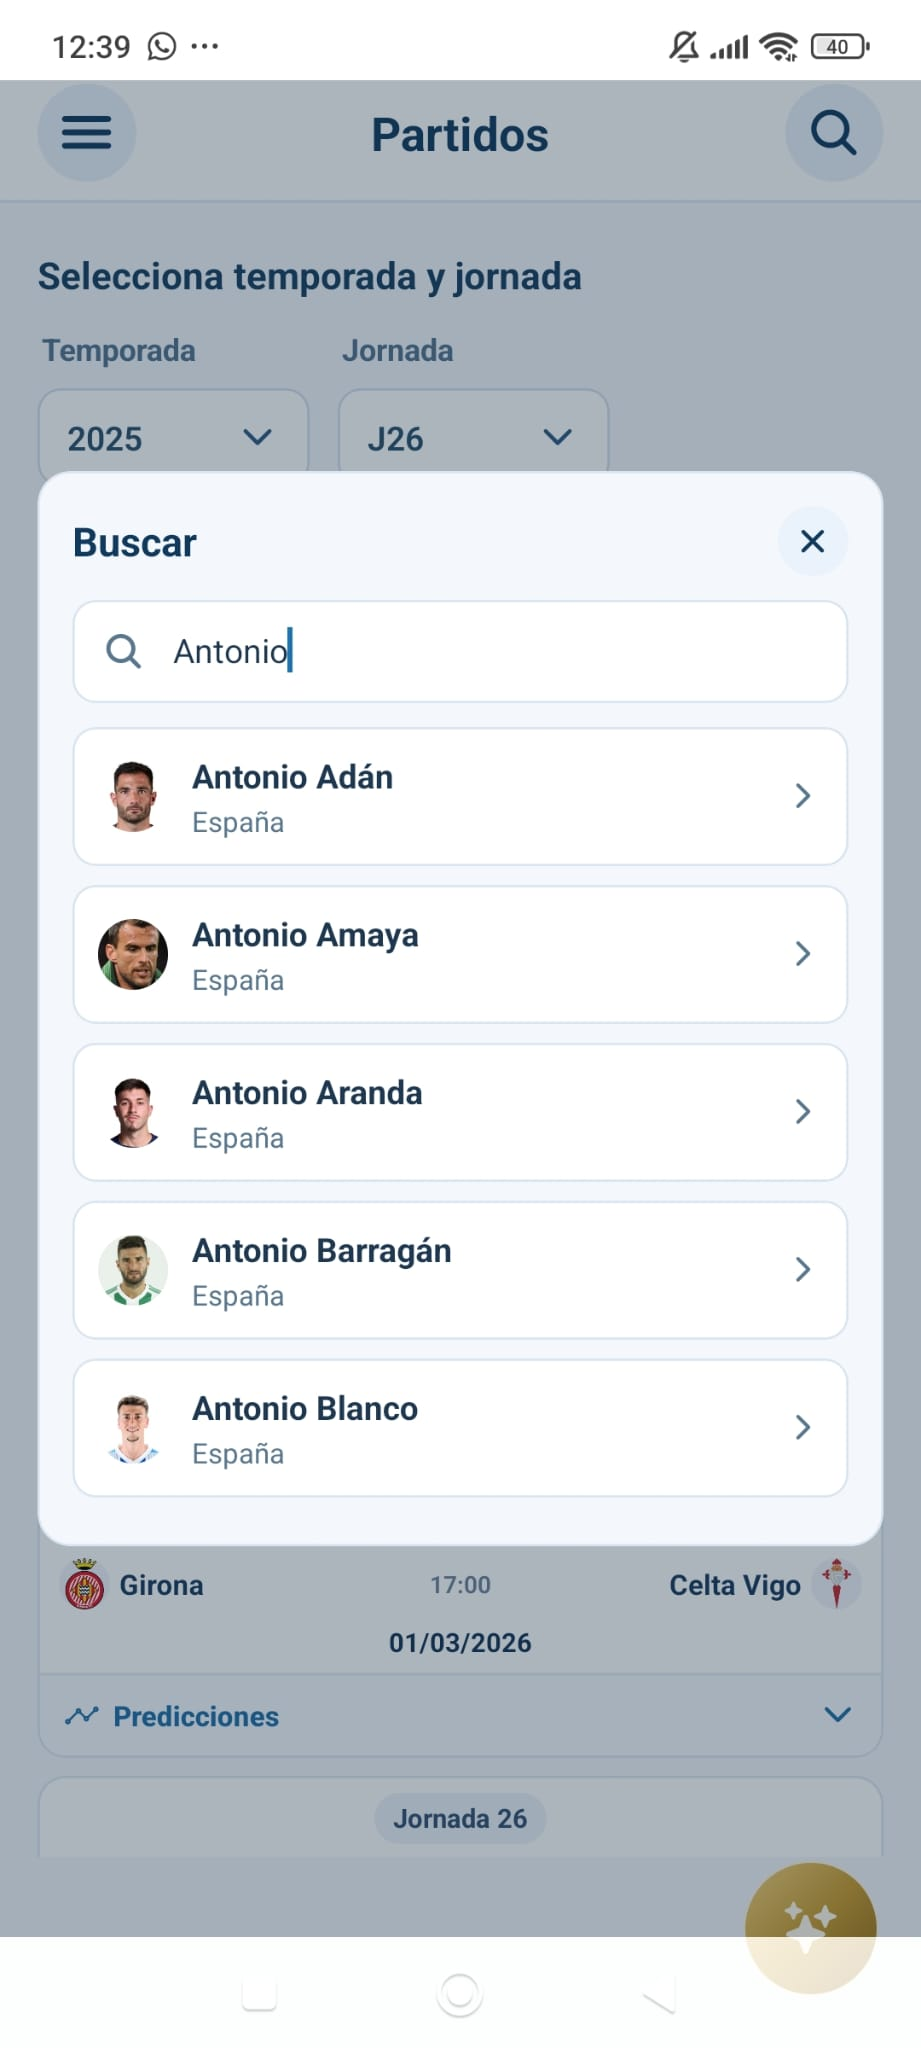
\includegraphics[width=0.5\textwidth]{figures/cap_buscador.jpeg}
\caption{Buscador}
\label{fig:buscador}
\end{subfigure}
\caption{Navegación y búsqueda dentro de la aplicación}
\label{fig:menu_buscador}
\end{figure}

Las pantallas de acceso y gestión de usuario permiten iniciar sesión, registrar una nueva cuenta y consultar o modificar los datos del perfil.

\begin{figure}[H]
\centering
\begin{subfigure}[b]{0.32\textwidth}
\centering
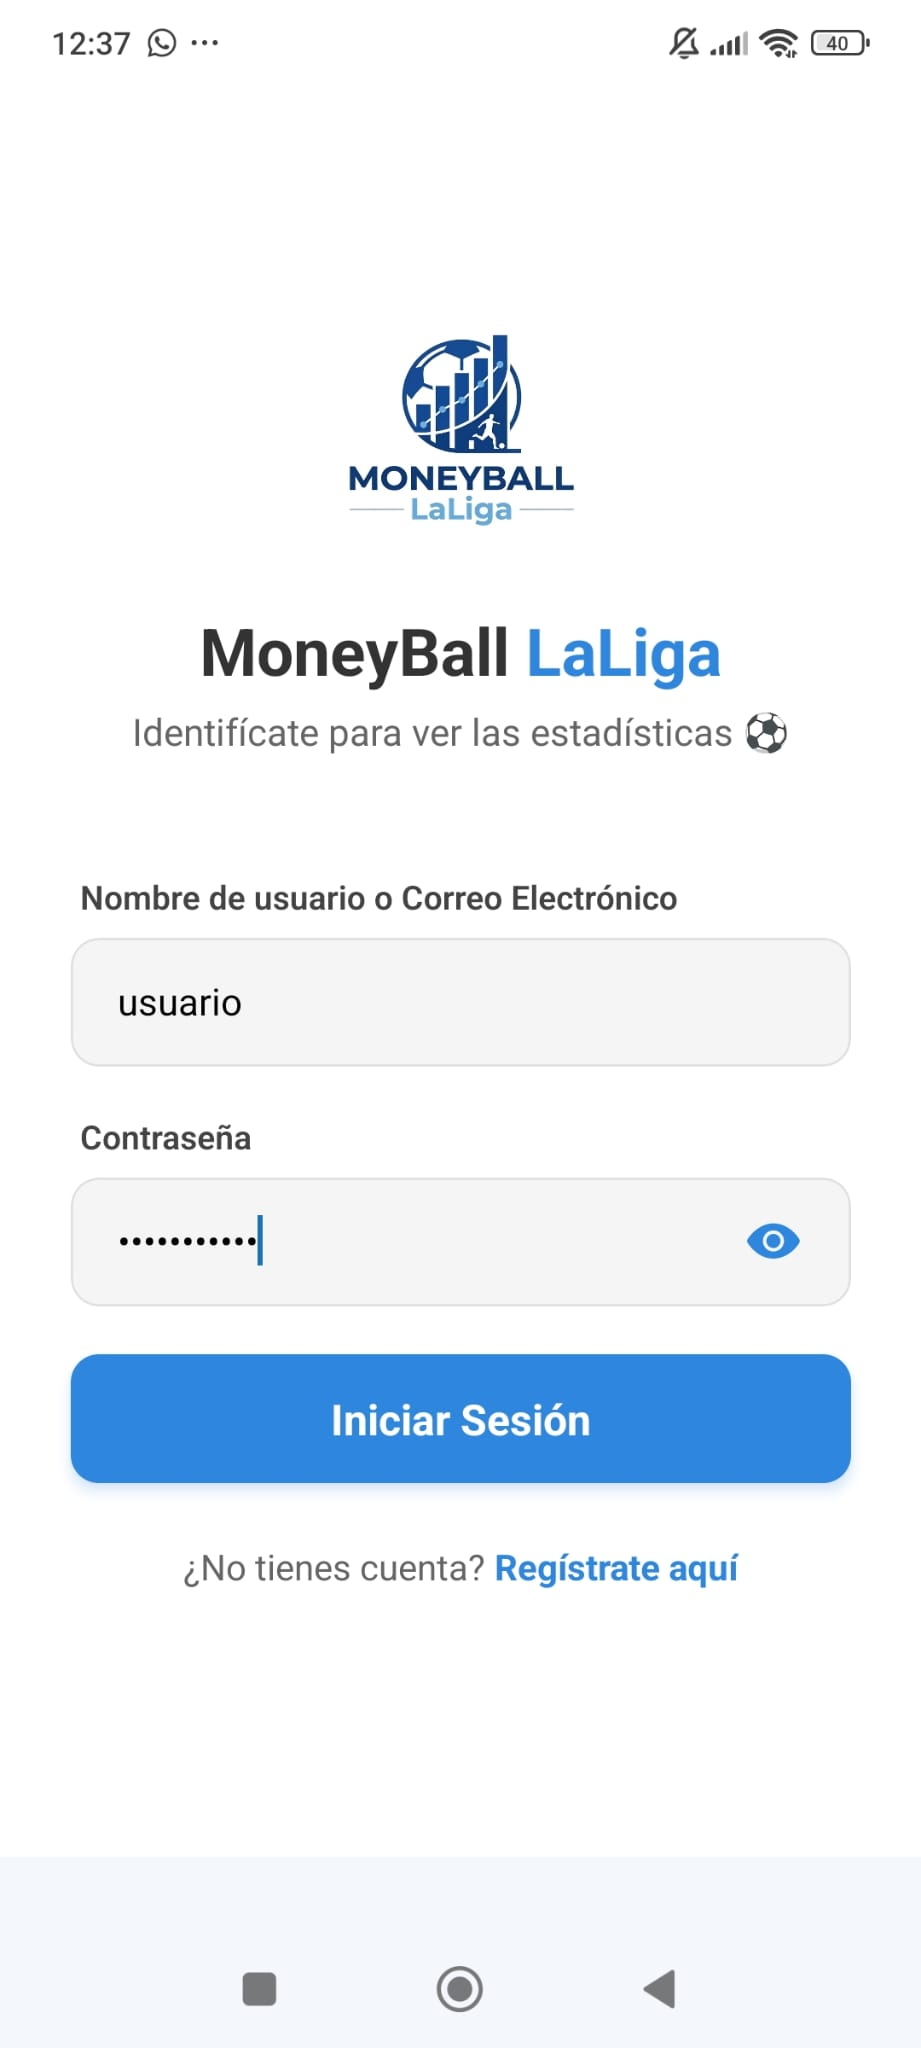
\includegraphics[width=0.8\textwidth]{figures/cap_iniciosesion.jpeg}
\caption{Inicio de sesión}
\label{fig:inicio_sesion}
\end{subfigure}
\hfill
\begin{subfigure}[b]{0.32\textwidth}
\centering
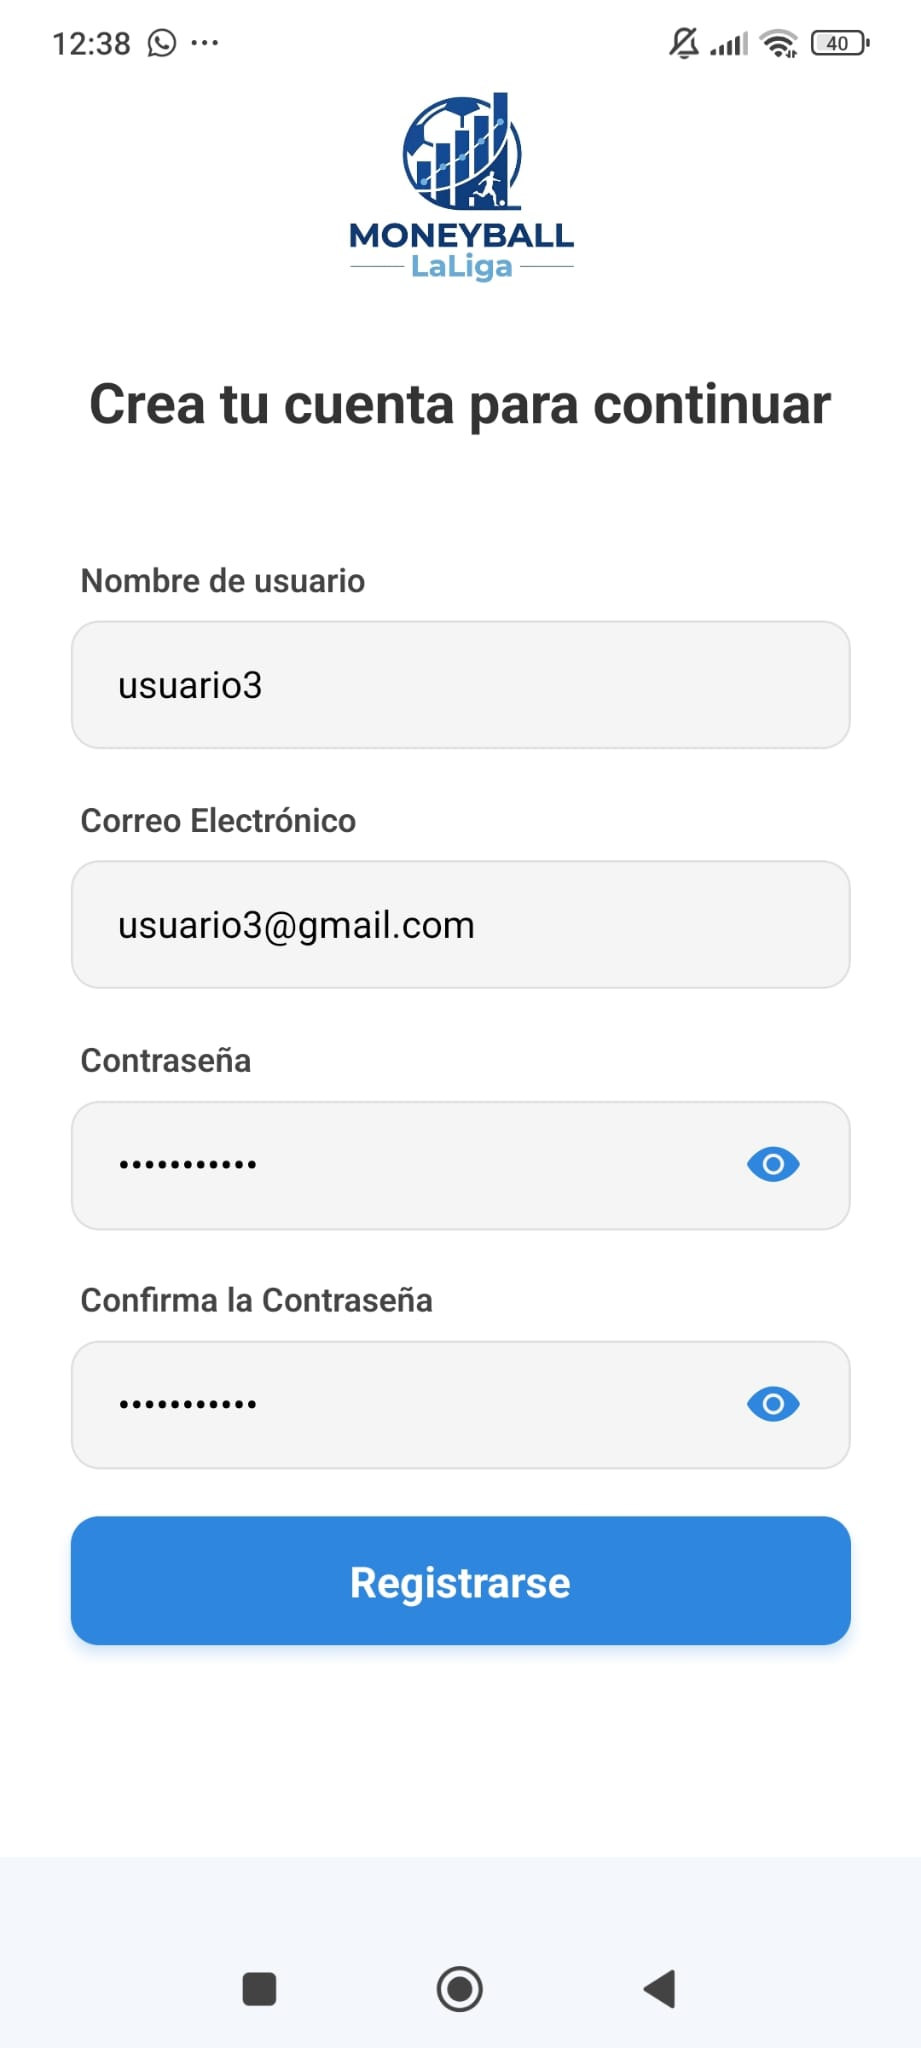
\includegraphics[width=0.8\textwidth]{figures/cap_registro.jpeg}
\caption{Registro}
\label{fig:registro}
\end{subfigure}
\hfill
\begin{subfigure}[b]{0.32\textwidth}
\centering
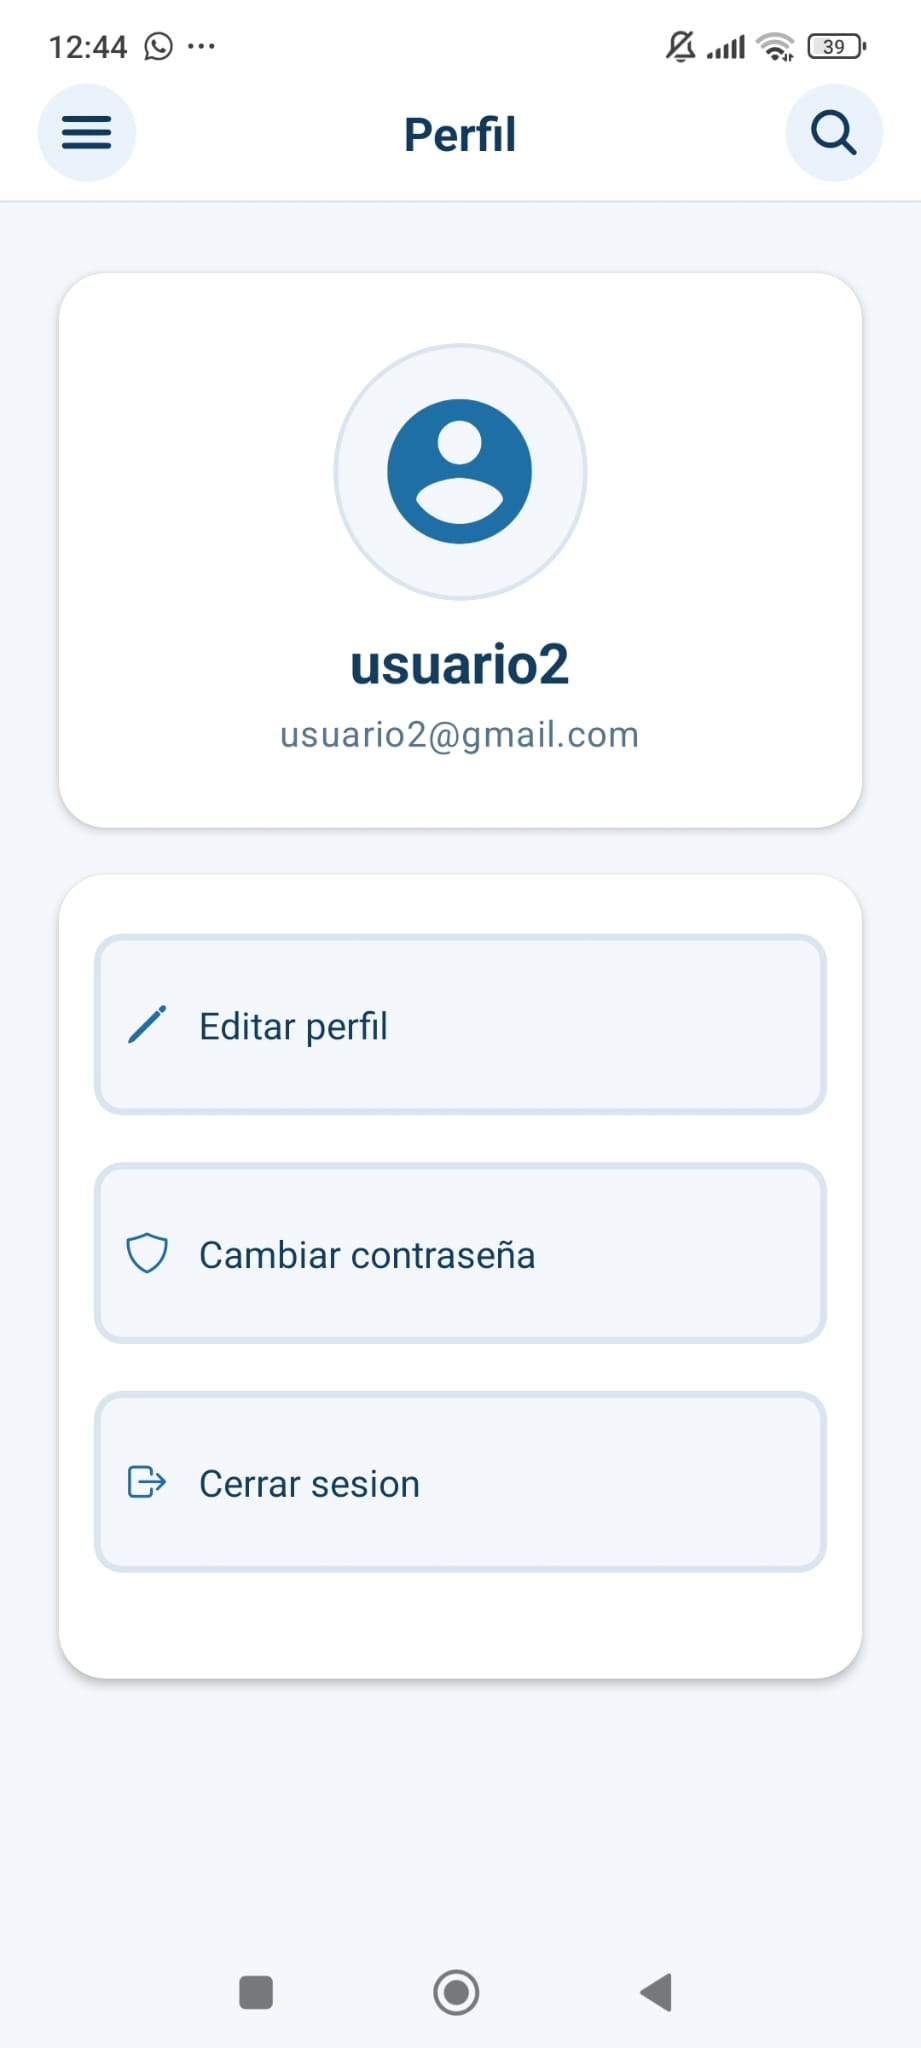
\includegraphics[width=0.8\textwidth]{figures/cap_perfil.jpeg}
\caption{Perfil}
\label{fig:perfil}
\end{subfigure}

\caption{Pantallas de acceso y gestión del usuario}
\label{fig:gestion_usuario}
\end{figure}

Las principales pantallas de consulta deportiva permiten acceder a jugadores, partidos y temporadas. Desde estas vistas se puede explorar la información almacenada en la base de datos y consultar estadísticas, eventos, clasificaciones y otros datos relevantes.

\begin{figure}[H]
\centering
\begin{subfigure}[b]{0.32\textwidth}
\centering
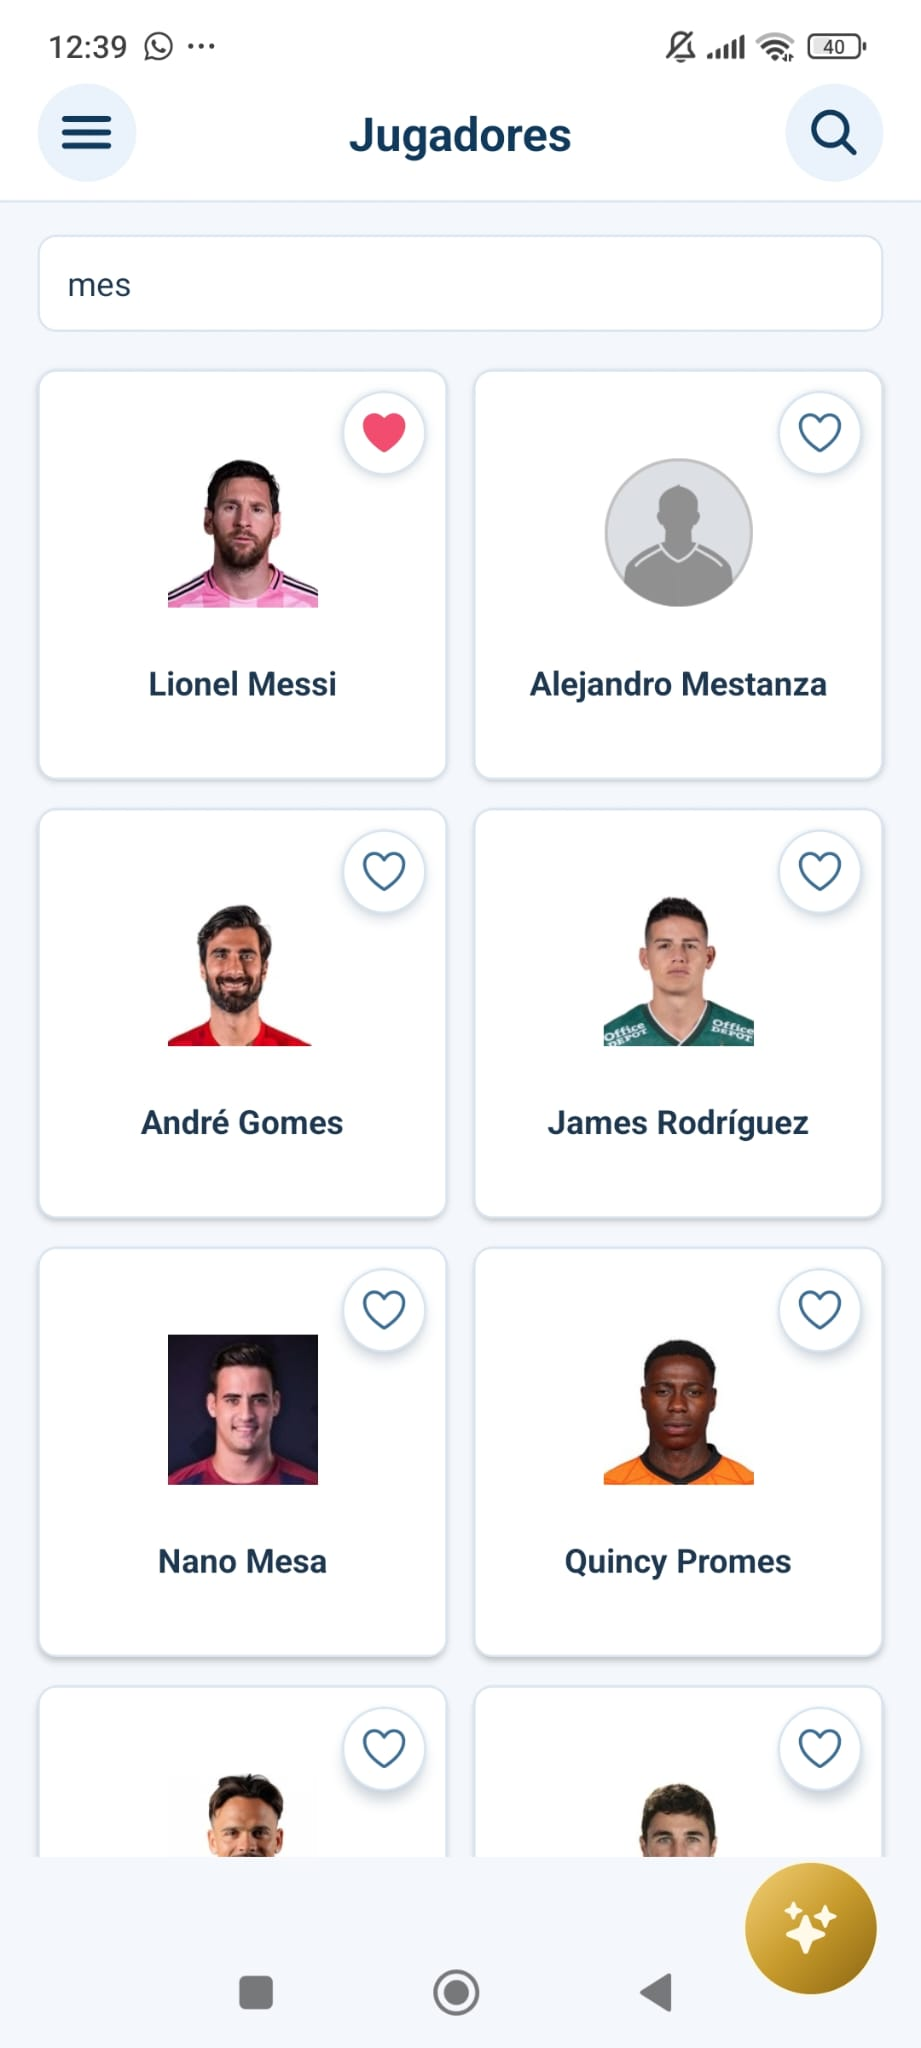
\includegraphics[width=0.8\textwidth]{figures/cap_jugadores.jpeg}
\caption{Jugadores}
\label{fig:jugadores}
\end{subfigure}
\hfill
\begin{subfigure}[b]{0.32\textwidth}
\centering
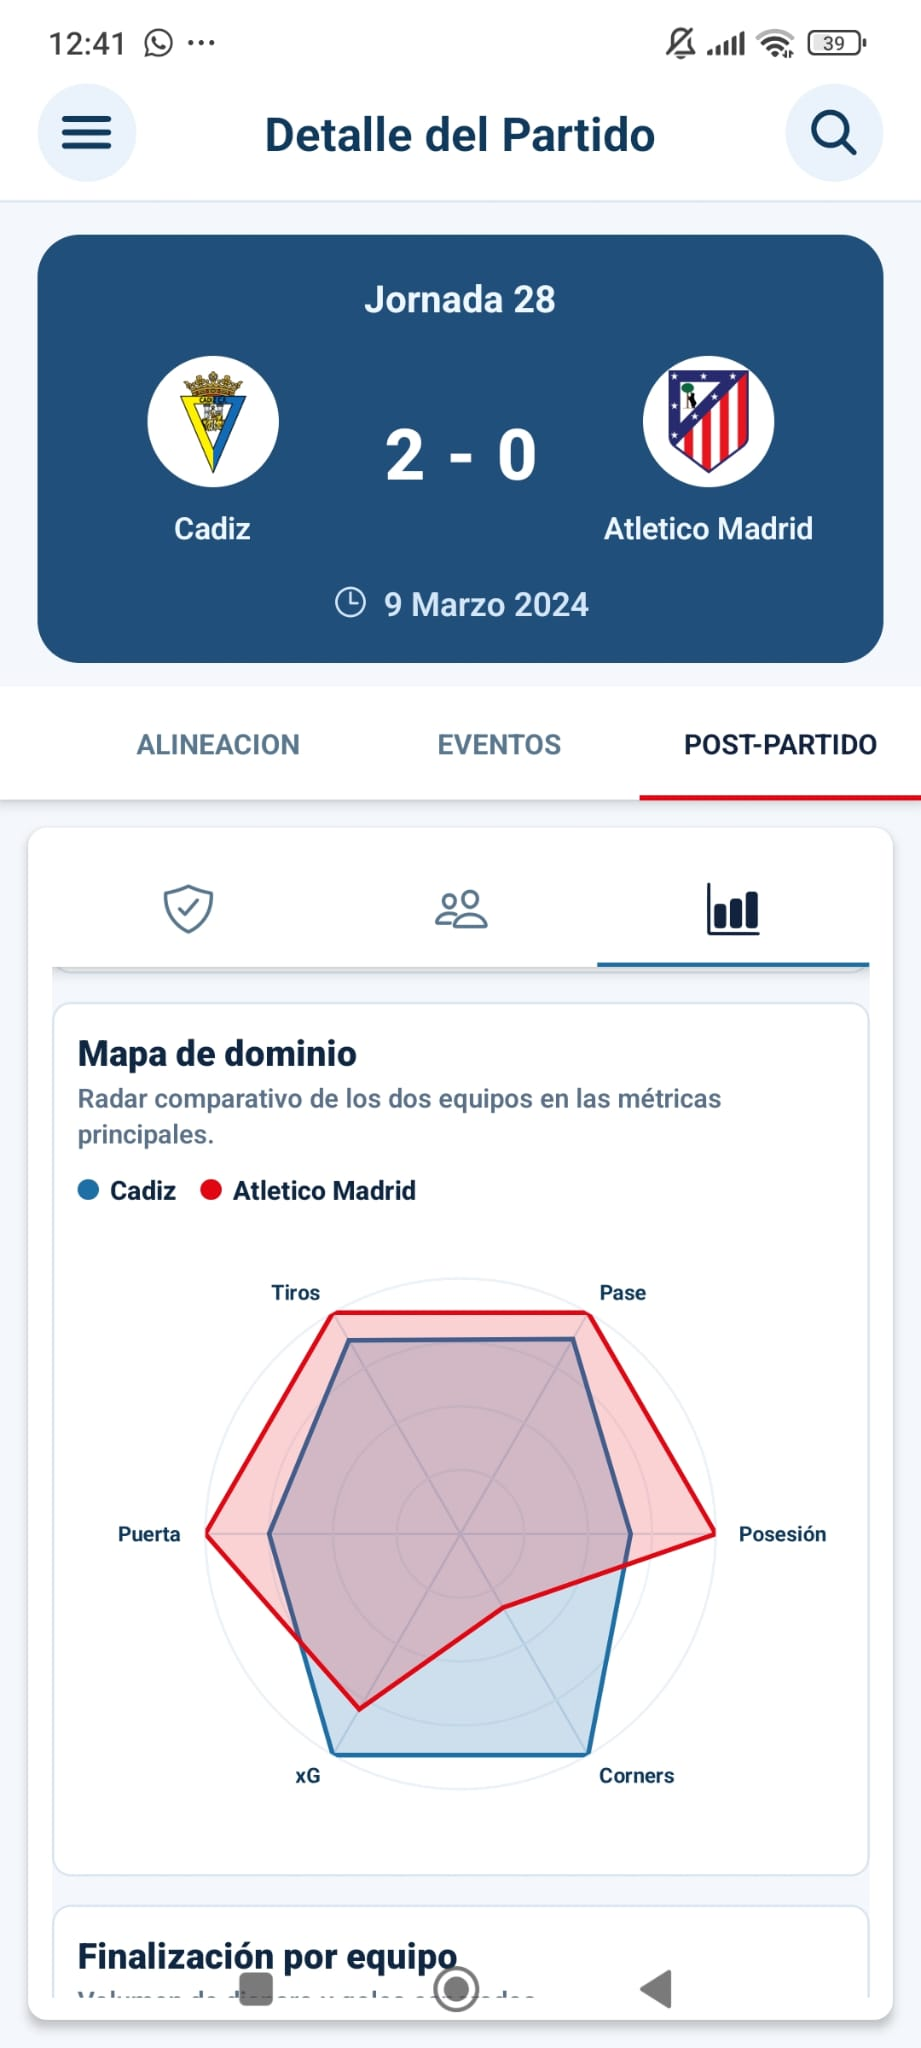
\includegraphics[width=0.8\textwidth]{figures/cap_dash_partido.jpeg}
\caption{Partido}
\label{fig:dashboard_partido}
\end{subfigure}
\hfill
\begin{subfigure}[b]{0.32\textwidth}
\centering
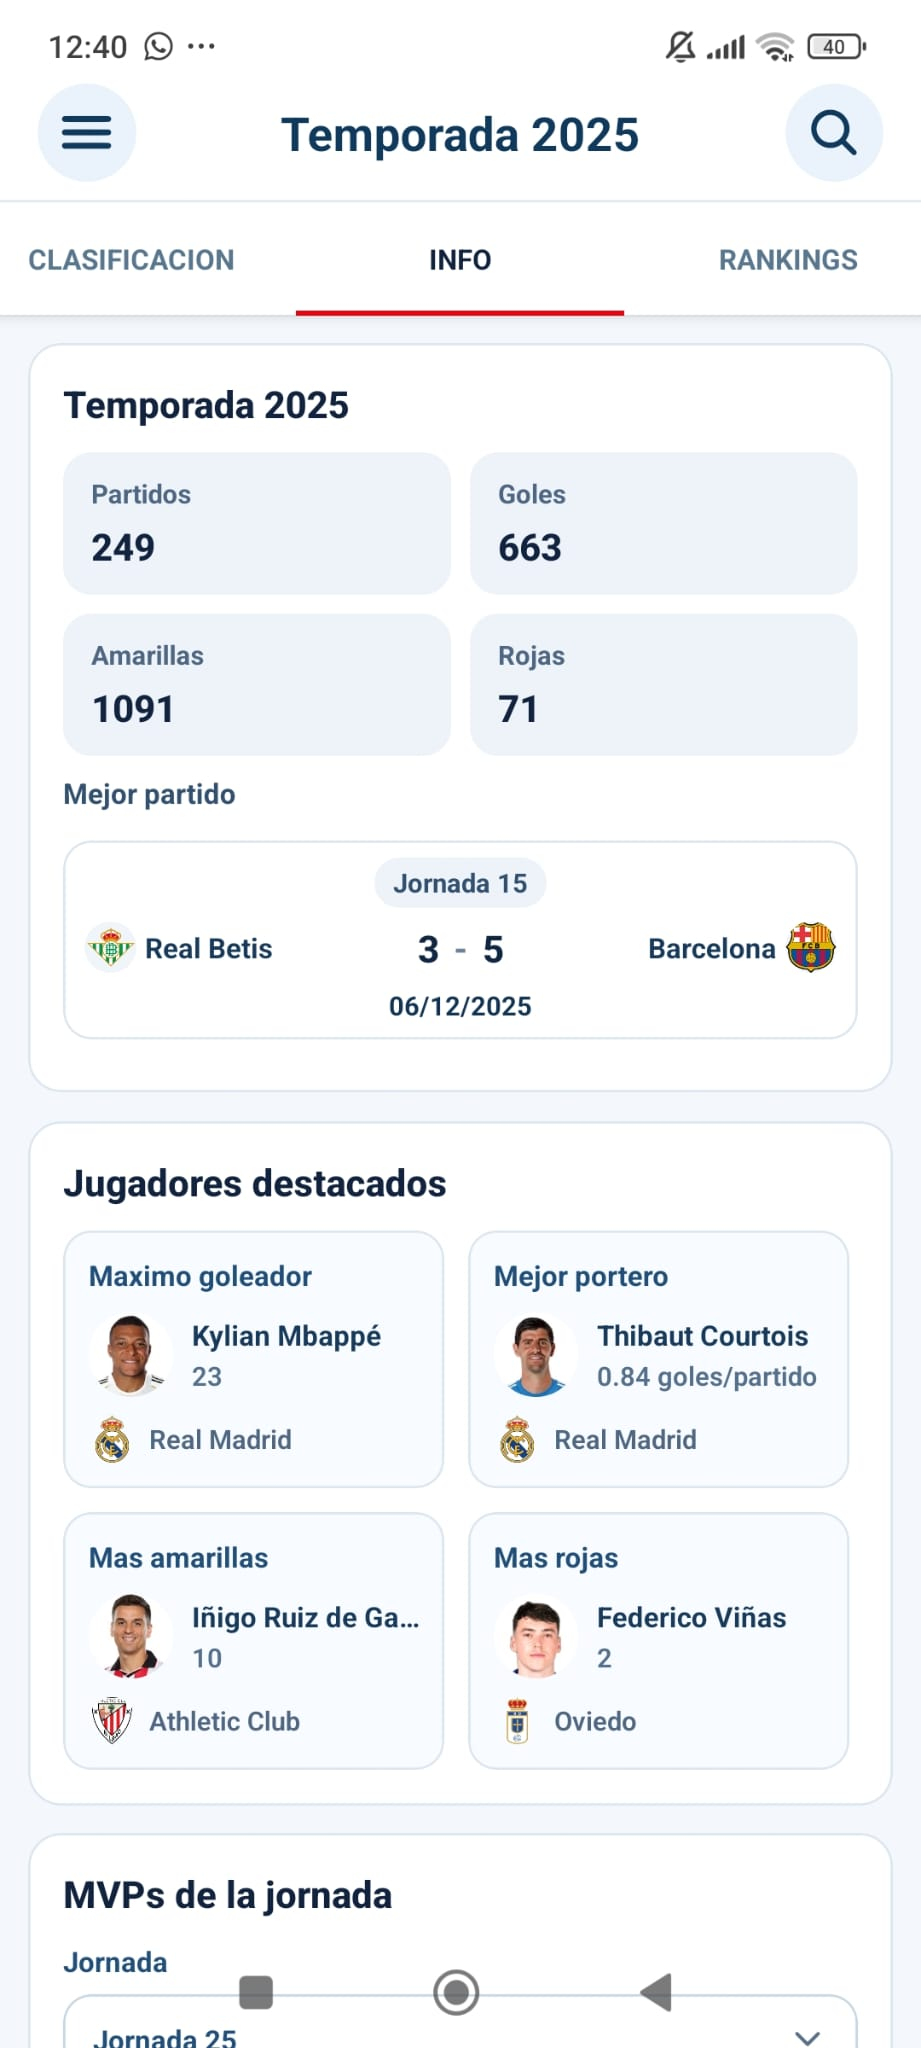
\includegraphics[width=0.8\textwidth]{figures/cap_tempo_inof.jpeg}
\caption{Temporada}
\label{fig:temporada}
\end{subfigure}

\caption{Principales pantallas de consulta deportiva}
\label{fig:consultas_deportivas}
\end{figure}

Entre las funcionalidades avanzadas se encuentran el análisis mediante inteligencia artificial y la simulación de temporadas. El módulo de inteligencia artificial permite generar información procesada a partir de los datos disponibles y guardar determinados análisis como favoritos.

\begin{figure}[H]
\centering
\begin{subfigure}[b]{0.4\textwidth}
\centering
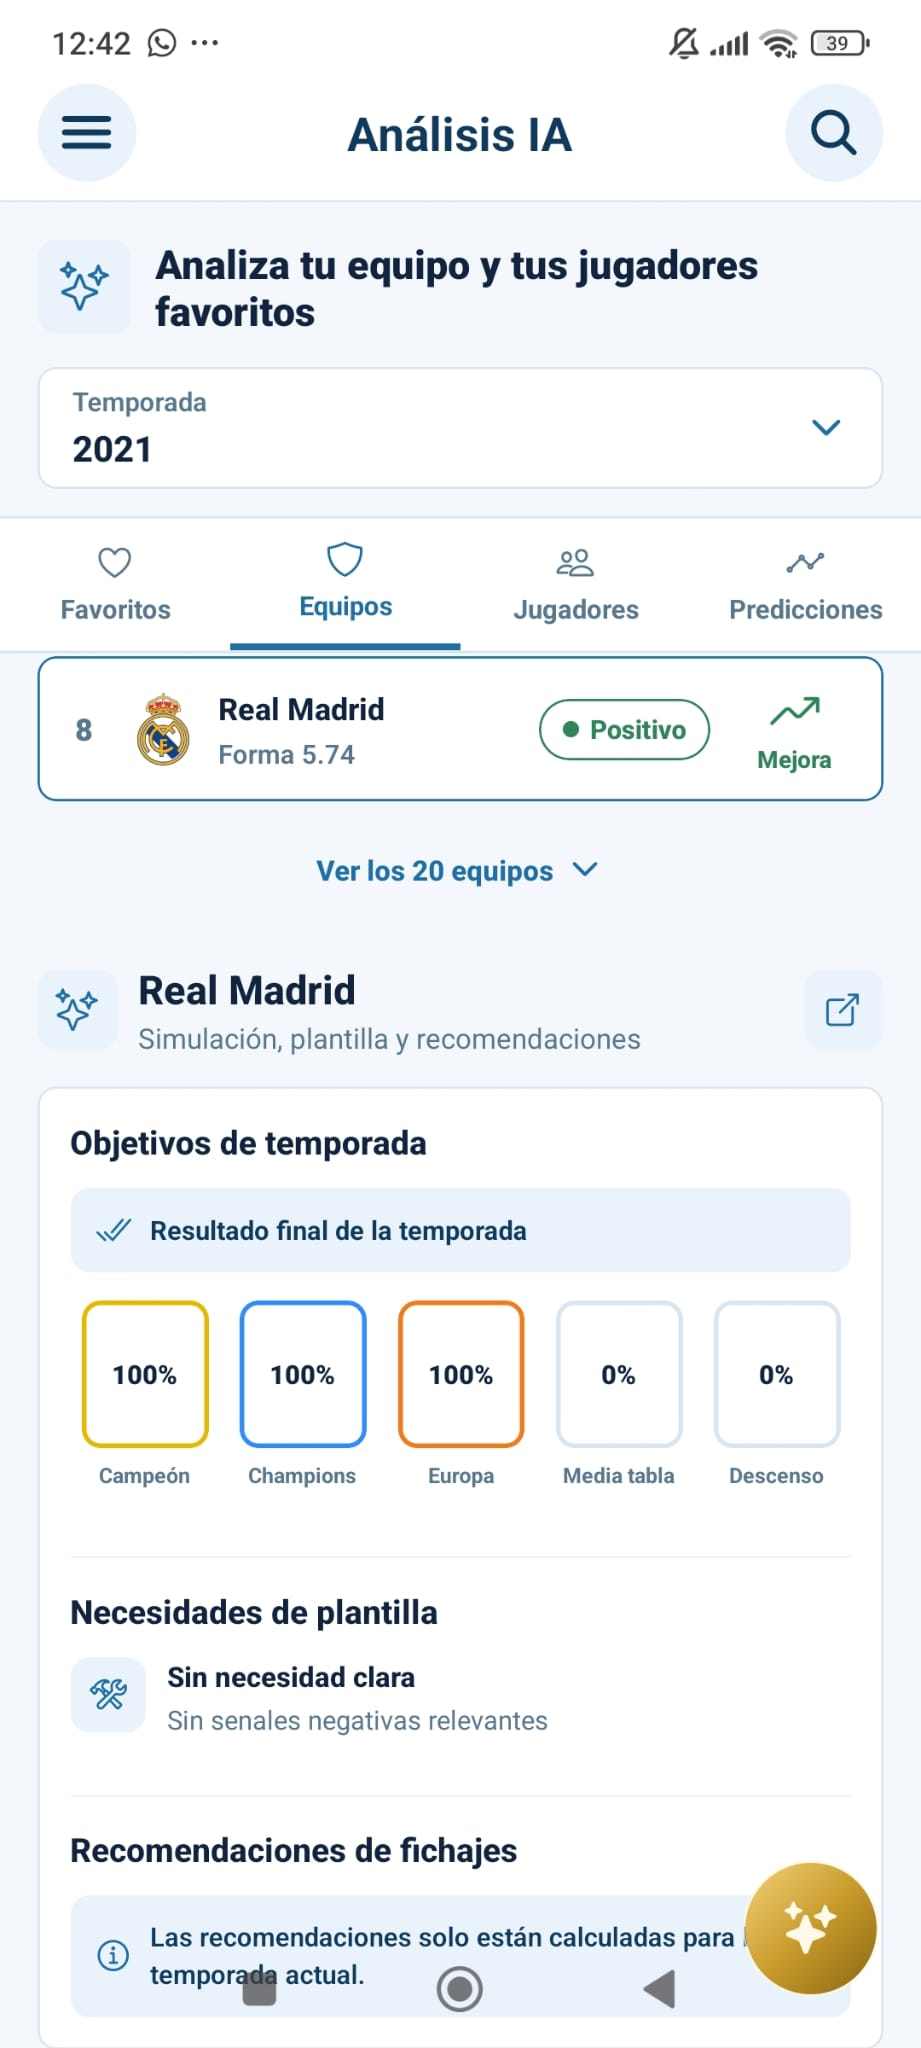
\includegraphics[width=0.5\textwidth]{figures/cap_analisisIA.jpeg}
\caption{Análisis mediante IA}
\label{fig:analisis_ia}
\end{subfigure}
%
\begin{subfigure}[b]{0.4\textwidth}
\centering
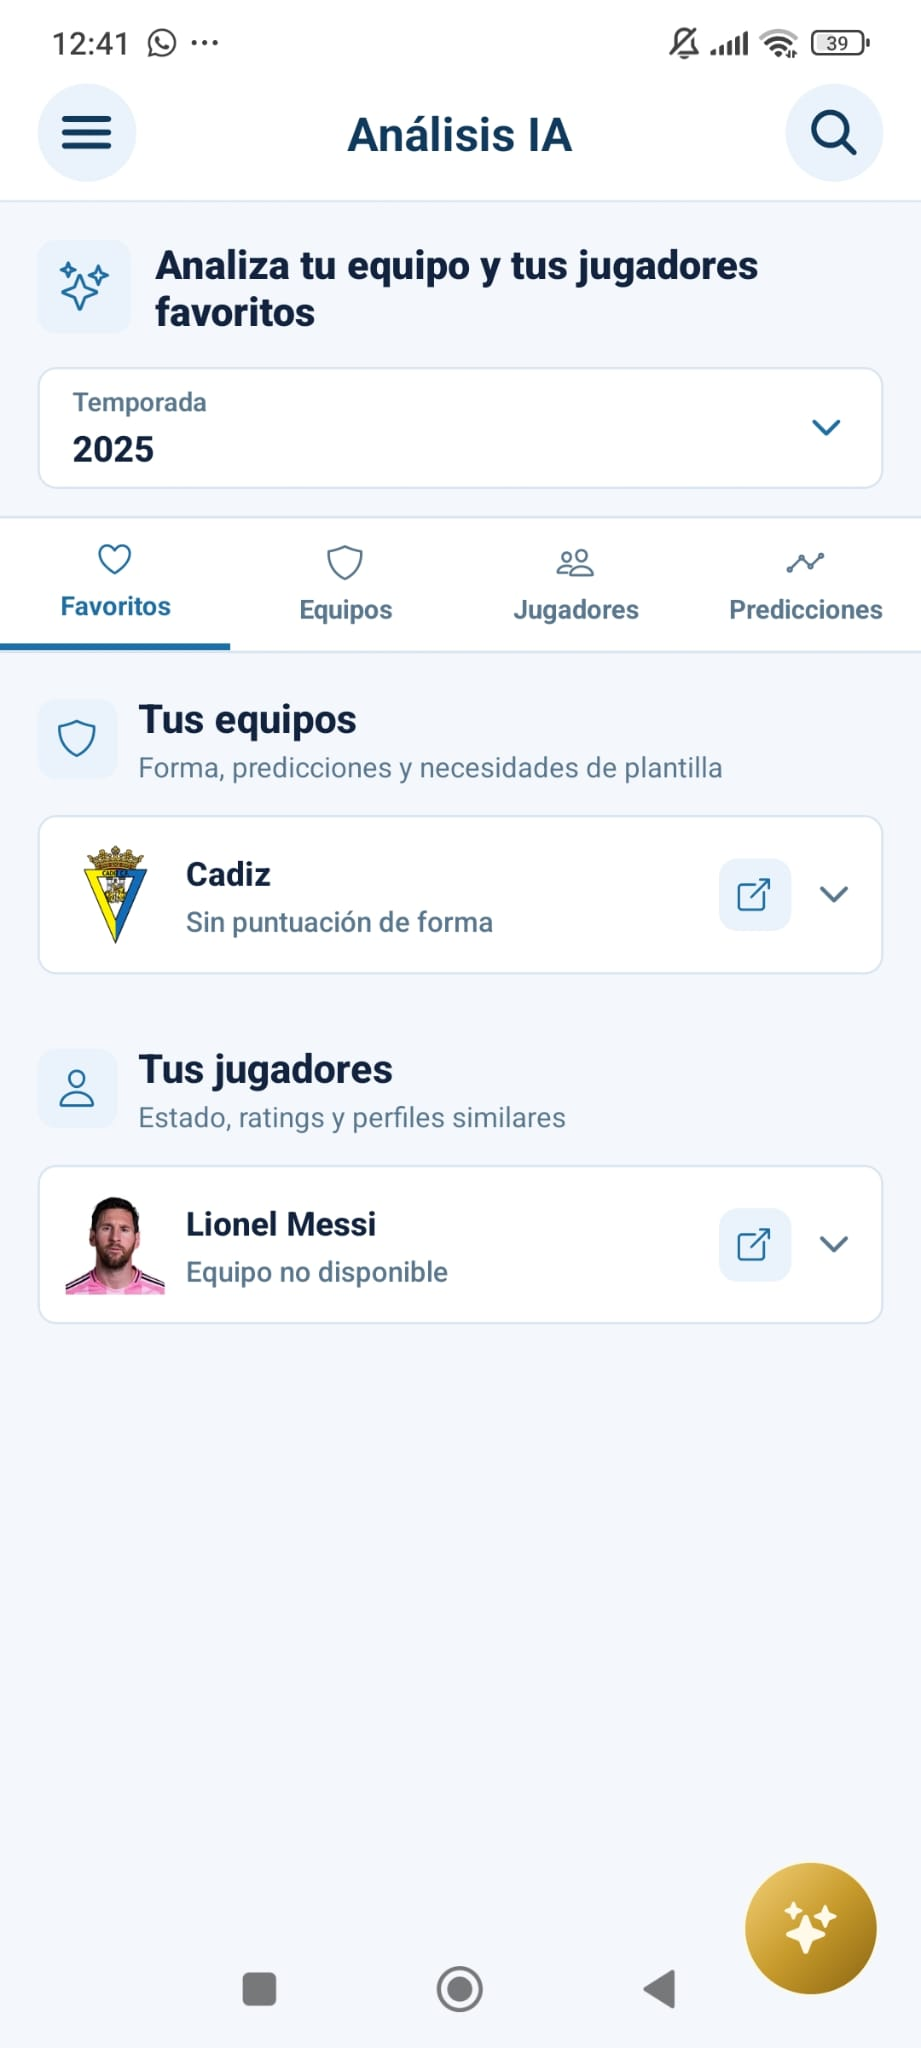
\includegraphics[width=0.5\textwidth]{figures/cap_analisisIA_Fav.jpeg}
\caption{Análisis guardado como favorito}
\label{fig:analisis_ia_fav}
\end{subfigure}
\caption{Funcionalidades de análisis mediante inteligencia artificial}
\label{fig:analisis_ia_general}
\end{figure}

La simulación permite analizar posibles escenarios futuros de la competición mediante el cálculo de probabilidades y la ejecución de simulaciones. El usuario puede consultar tanto la clasificación simulada como las probabilidades empleadas y los resultados finales obtenidos.

\begin{figure}[H]
\centering
\begin{subfigure}[b]{0.32\textwidth}
\centering
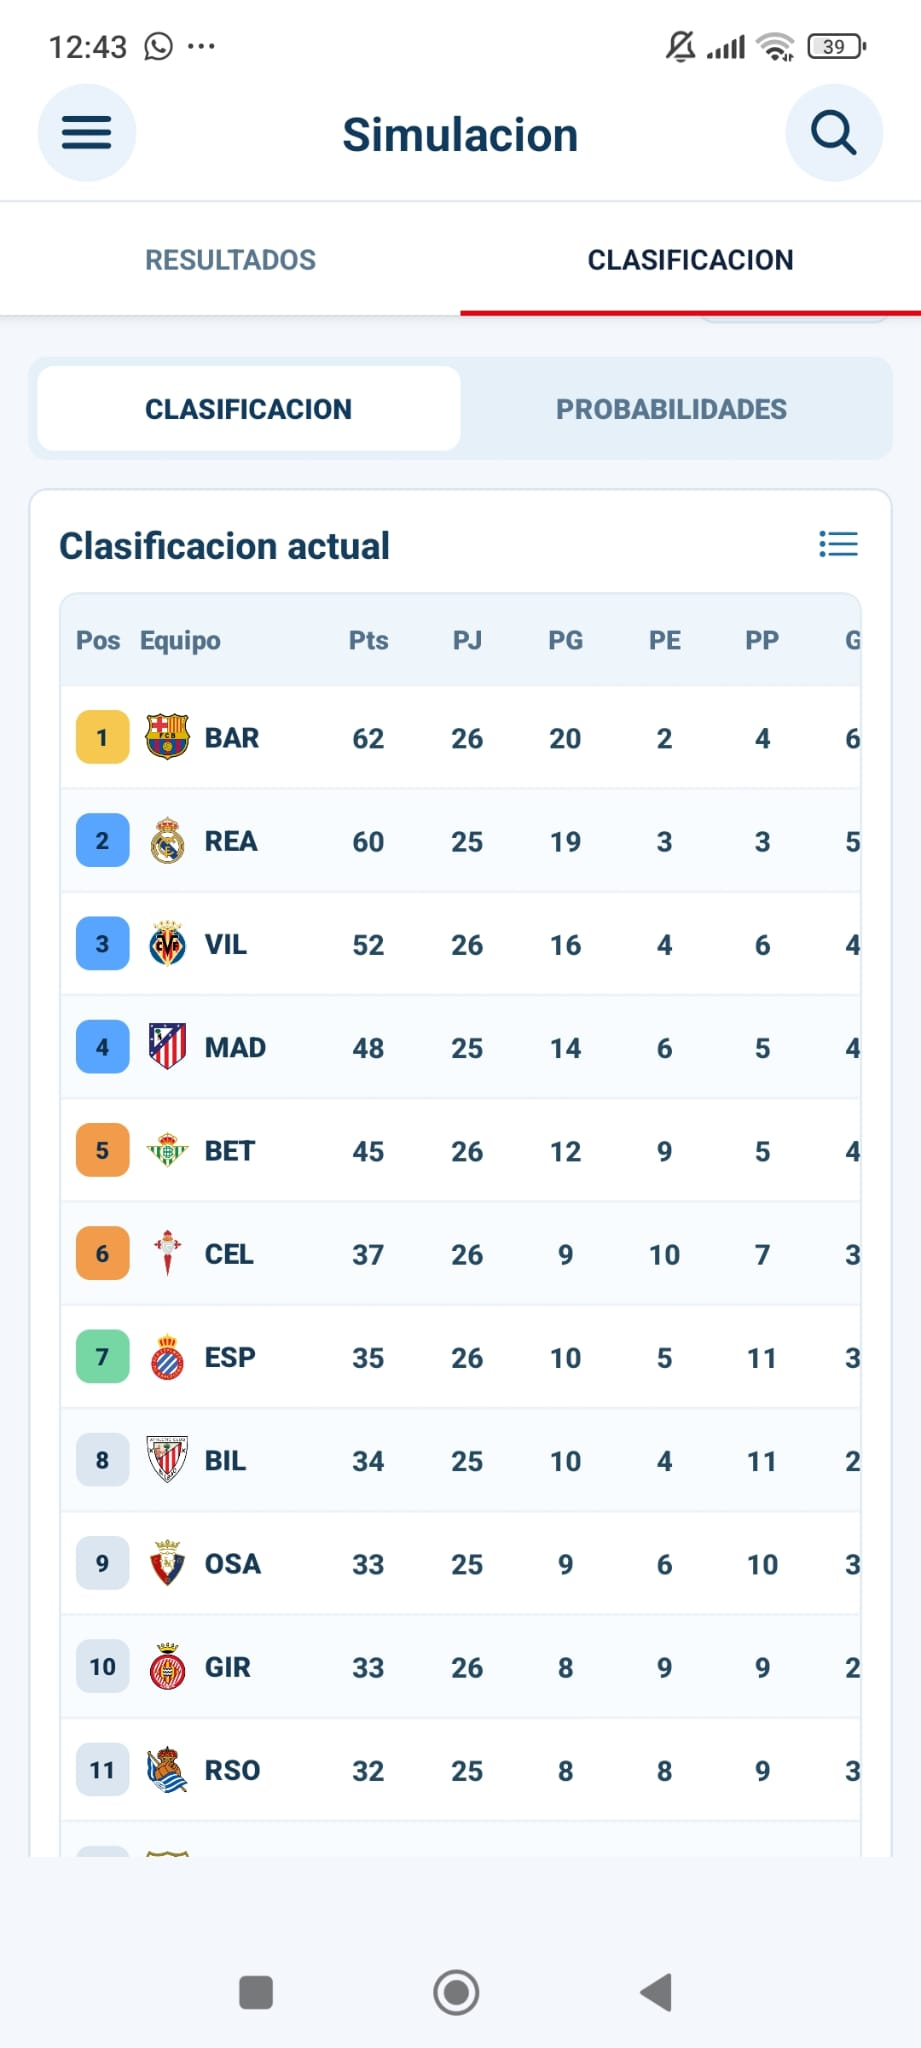
\includegraphics[width=0.8\textwidth]{figures/cap_sim_clasi.jpeg}
\caption{Clasificación simulada}
\label{fig:sim_clasi}
\end{subfigure}
\hfill
\begin{subfigure}[b]{0.32\textwidth}
\centering
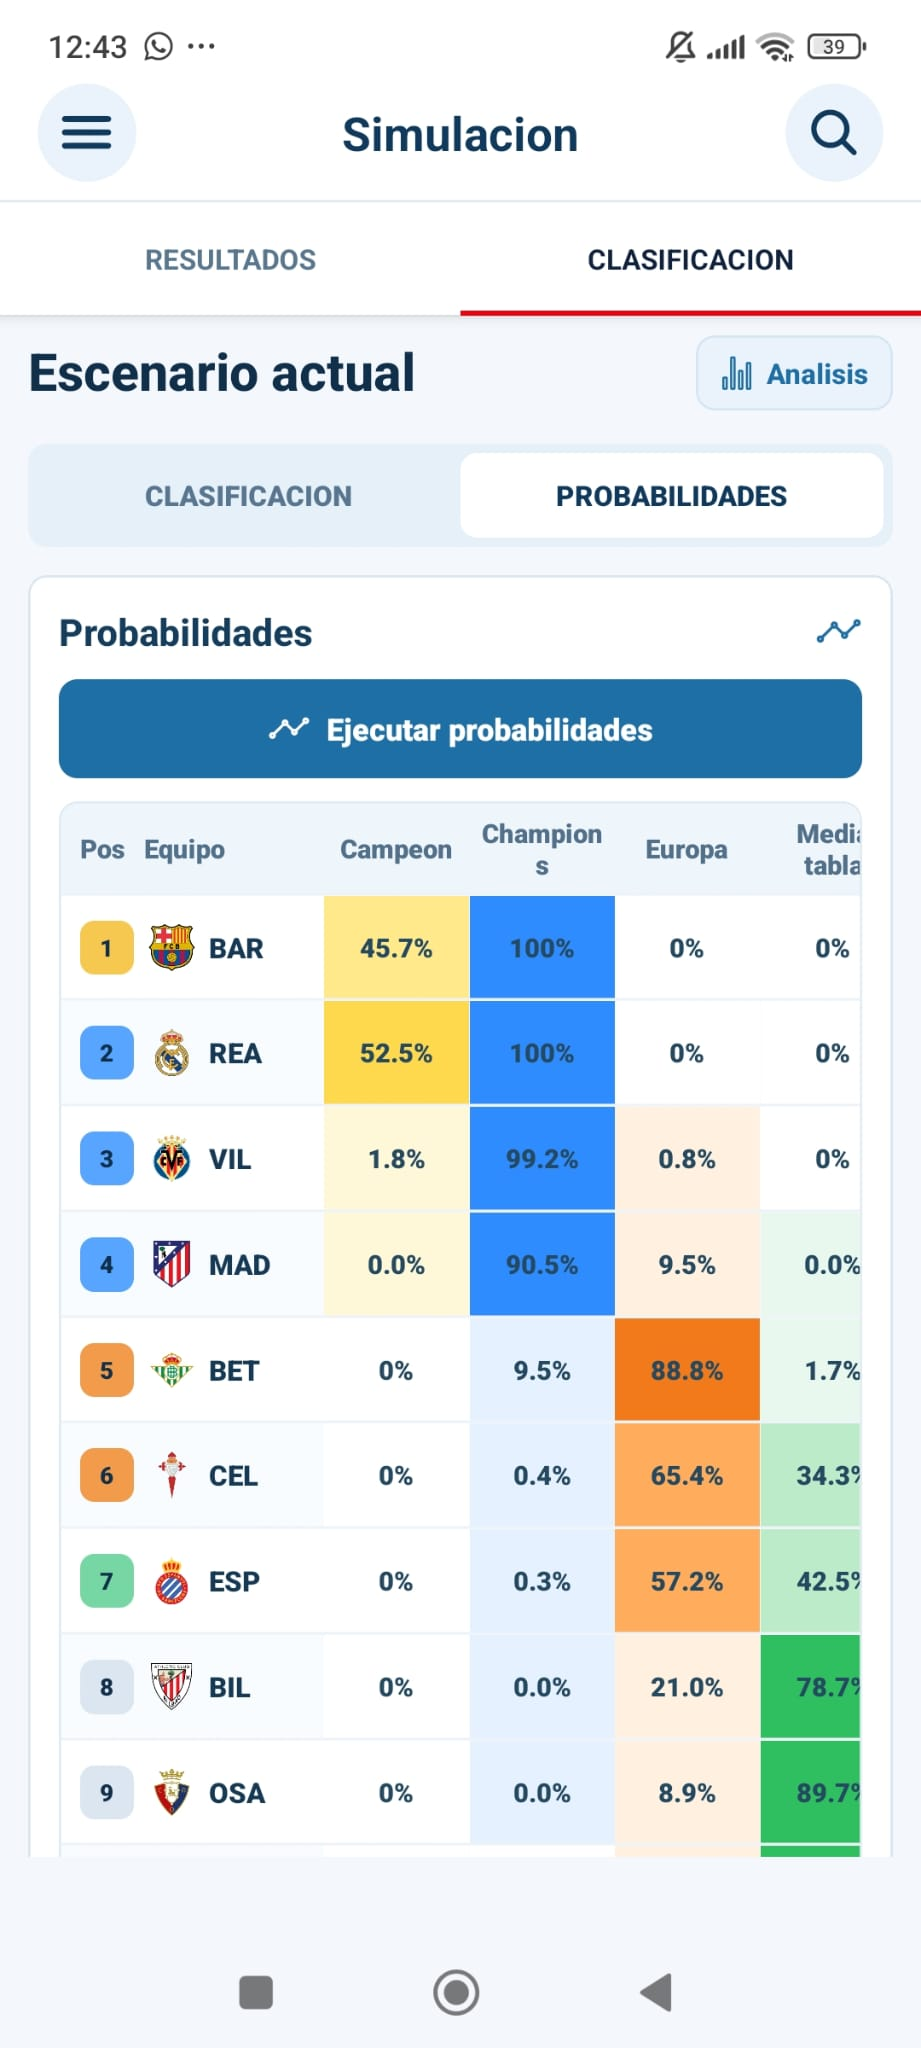
\includegraphics[width=0.8\textwidth]{figures/cap_sim_prob.jpeg}
\caption{Probabilidades}
\label{fig:sim_prob}
\end{subfigure}
\hfill
\begin{subfigure}[b]{0.32\textwidth}
\centering
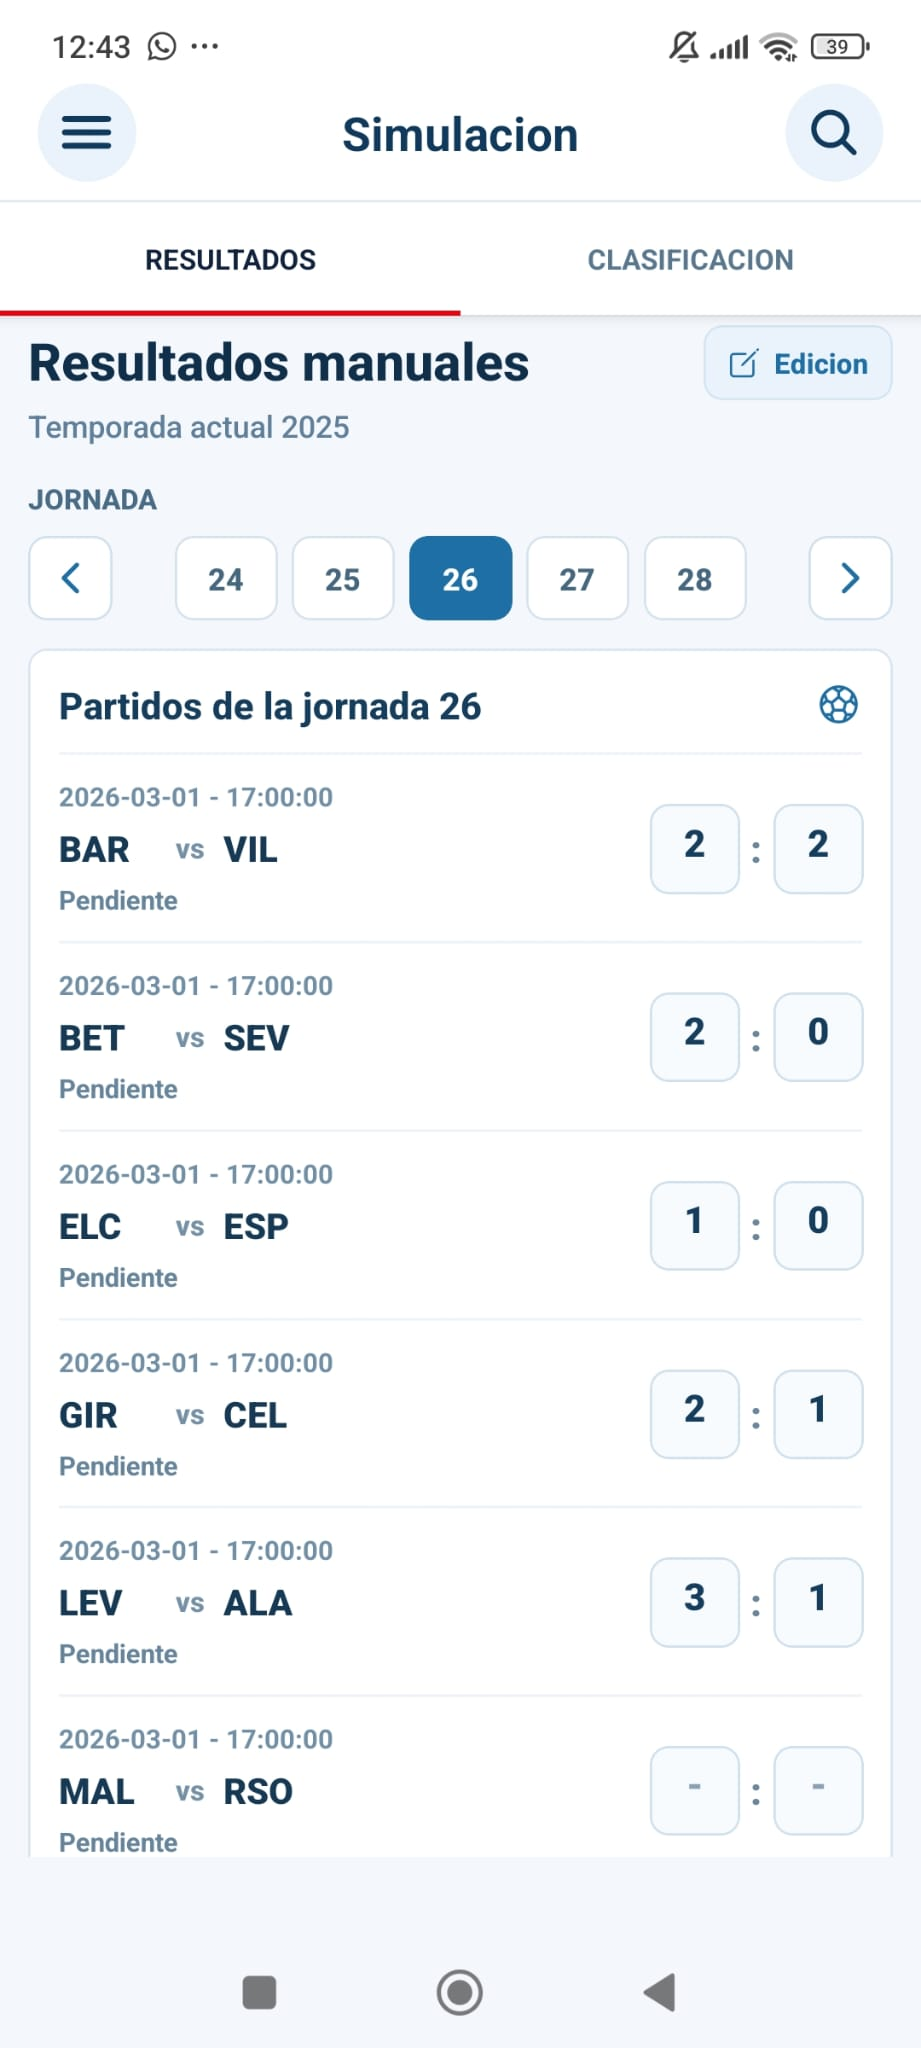
\includegraphics[width=0.8\textwidth]{figures/cap_sim_result.jpeg}
\caption{Resultados}
\label{fig:sim_result}
\end{subfigure}

\caption{Pantallas correspondientes al proceso de simulación}
\label{fig:simulacion}
\end{figure}

Por último, la aplicación incluye diferentes opciones de configuración y personalización de la cuenta, entre ellas la actualización de la contraseña y la adaptación de la interfaz mediante los temas claro y oscuro.

\begin{figure}[H]
\centering
\begin{subfigure}[b]{0.4\textwidth}
\centering
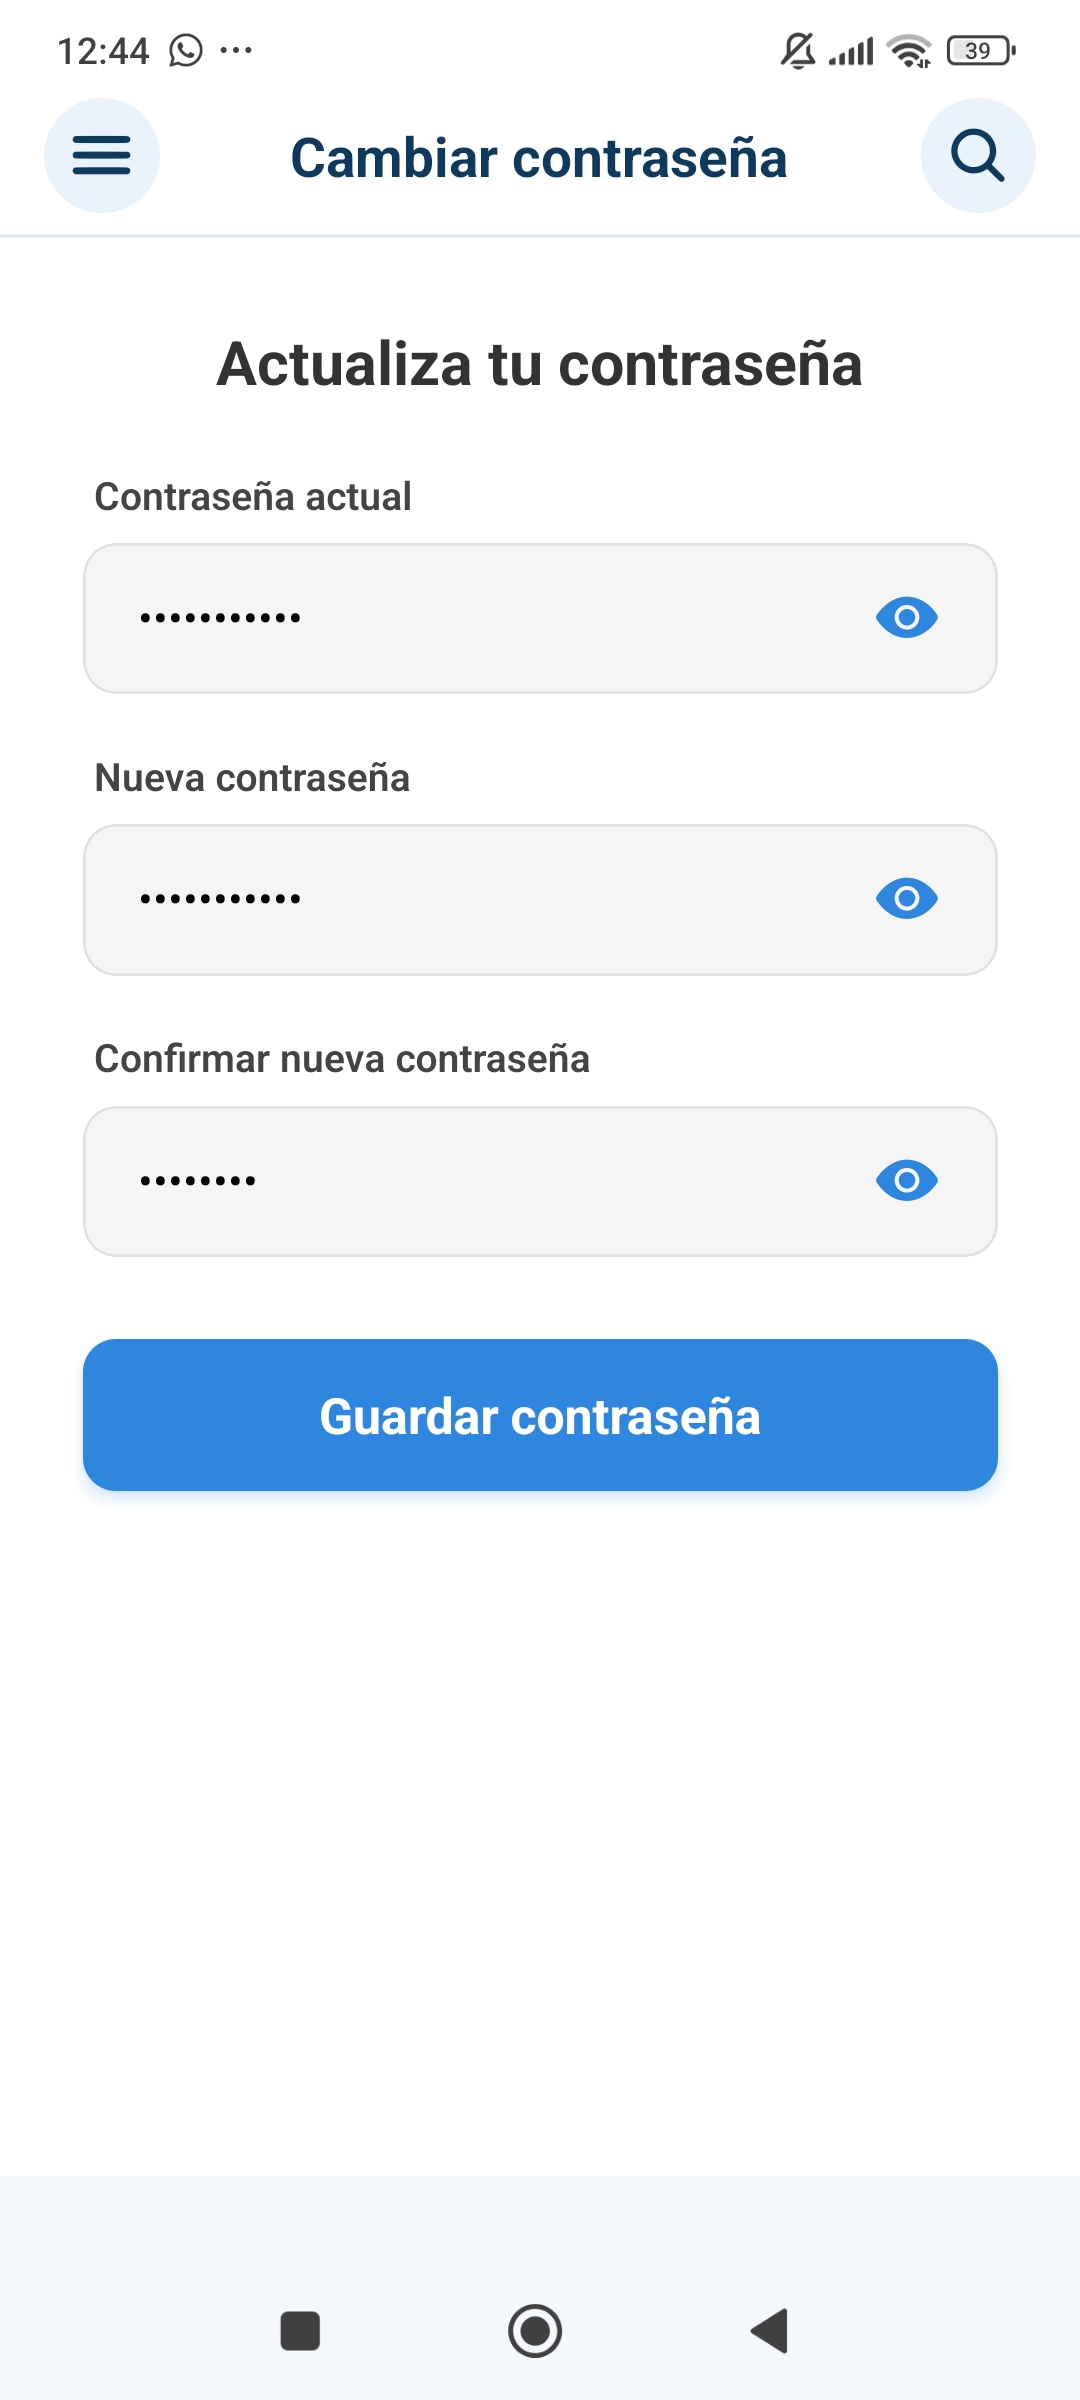
\includegraphics[width=0.5\textwidth]{figures/cap_act_contr.jpeg}
\caption{Actualización de contraseña}
\label{fig:actualizar_contrasena}
\end{subfigure}
\caption{Gestión y configuración de la cuenta}
\label{fig:configuracion}
\end{figure}

\subsection{Logotipo, colores y nombre de la aplicación}

El nombre de la aplicación, \textit{MoneyBall LaLiga}, toma como referencia la película \textit{Moneyball}, basada en la aplicación de métodos estadísticos y analíticos al ámbito deportivo. En dicha obra se muestra cómo el uso de datos puede ayudar a construir un equipo competitivo con recursos económicos limitados, identificando jugadores infravalorados a partir de indicadores objetivos de rendimiento. Esta idea se relaciona directamente con la finalidad del presente Trabajo Fin de Grado, ya que la aplicación busca facilitar el análisis de datos futbolísticos y apoyar la interpretación del rendimiento de equipos y jugadores. Además, se incorpora el término \textit{LaLiga} debido a que el proyecto se centra exclusivamente en esta competición.

En cuanto al logotipo, mostrado en la Figura~\ref{fig:logo}, se diseñó con apoyo de una herramienta de generación de imágenes basada en inteligencia artificial. Para su creación se partió de la idea de una aplicación denominada \textit{MoneyBall LaLiga}, utilizando tonos azules y una representación sencilla de elementos relacionados con gráficos y análisis de datos. El objetivo era obtener una imagen visual sobria, minimalista y coherente con el carácter analítico de la aplicación, evitando un diseño excesivamente recargado.

\begin{figure}[H]
    \centering
    
\includegraphics[width=0.6\linewidth]{figures/logo.png}
    \caption{Logo de la app.}
    \label{fig:logo}
\end{figure}

A partir de esta identidad visual se seleccionó una paleta principal basada en tonos azules. Esta elección busca transmitir una imagen tecnológica, limpia y profesional, manteniendo al mismo tiempo un contraste adecuado para los distintos elementos de la interfaz. La paleta fue elaborada mediante la herramienta Coolors y se muestra en la Figura~\ref{fig:paleta}.

\begin{figure}[H]
    \centering
    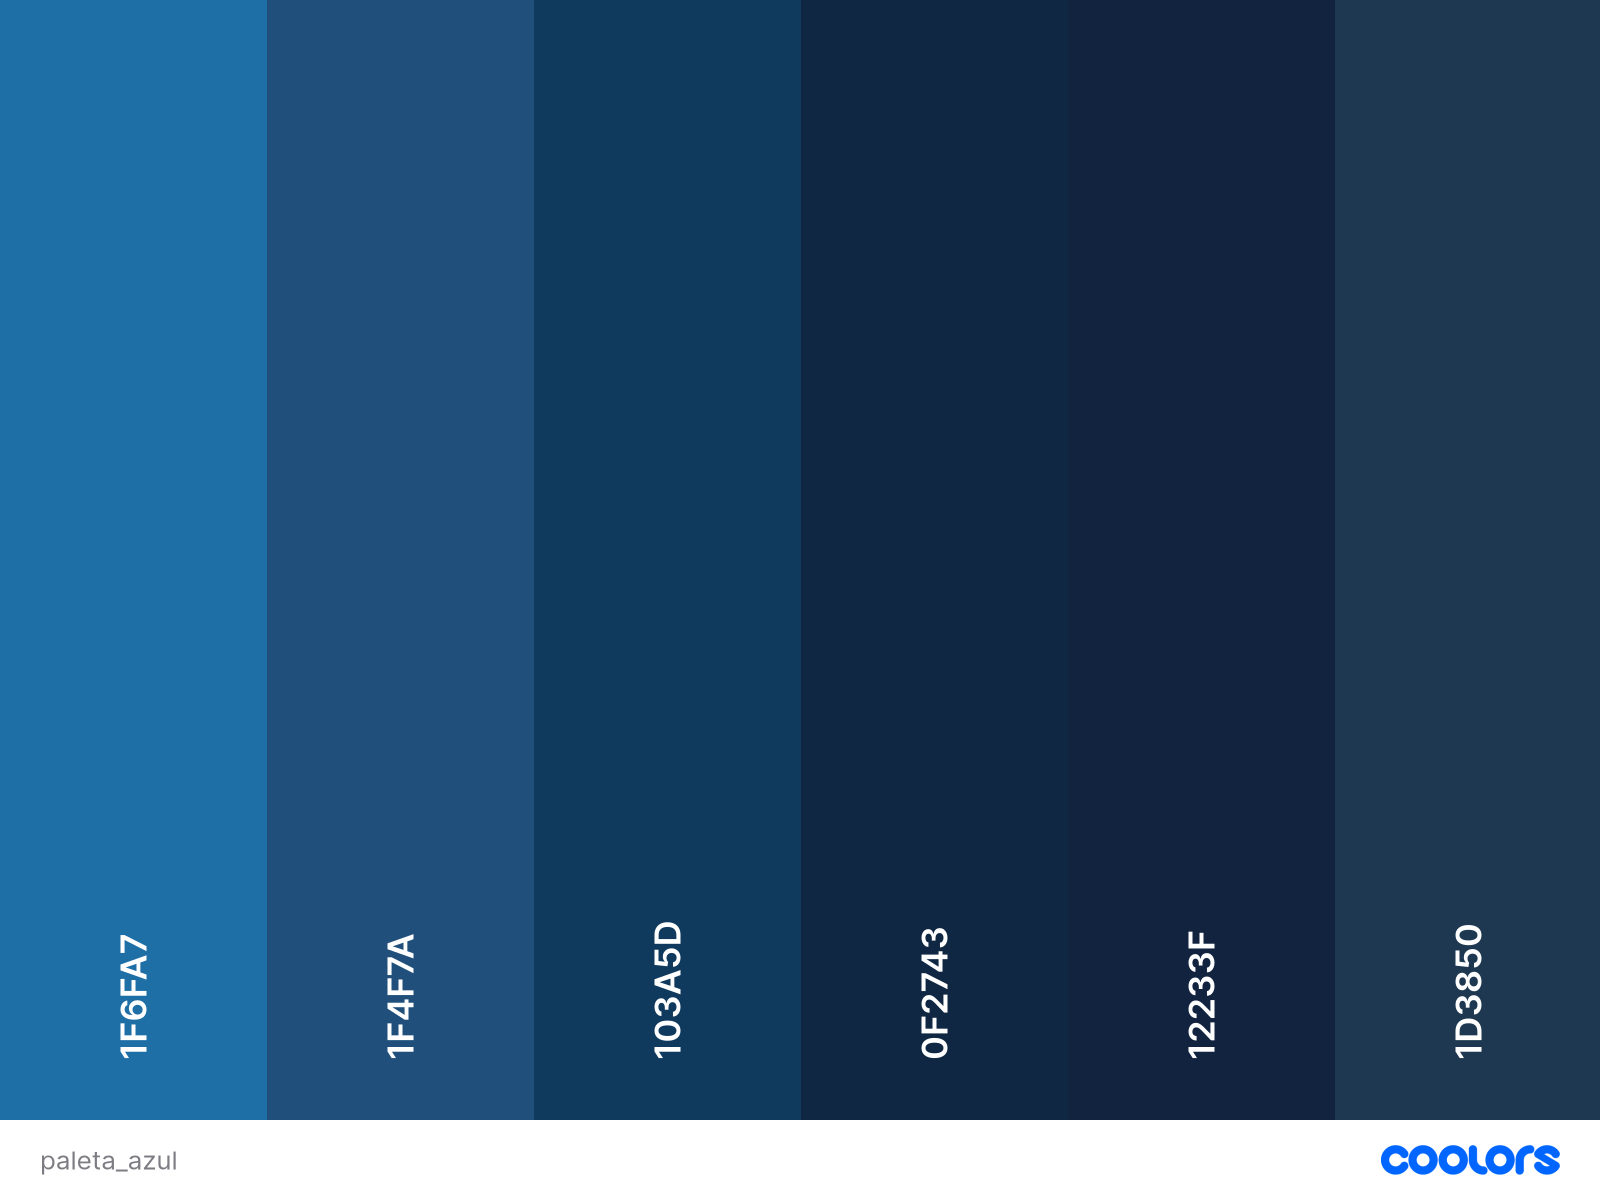
\includegraphics[width=0.8\linewidth]{figures/paleta_azul.png}
    \caption{Paleta de colores.}
    \label{fig:paleta}
\end{figure}

Para los fondos de la aplicación se escogió una combinación de colores claros y suaves, con el objetivo de favorecer la legibilidad y resaltar el azul principal utilizado en botones, encabezados y elementos interactivos. Esta paleta complementaria puede observarse en la Figura~\ref{fig:paleta_fondo}.

\begin{figure}[H]
    \centering
    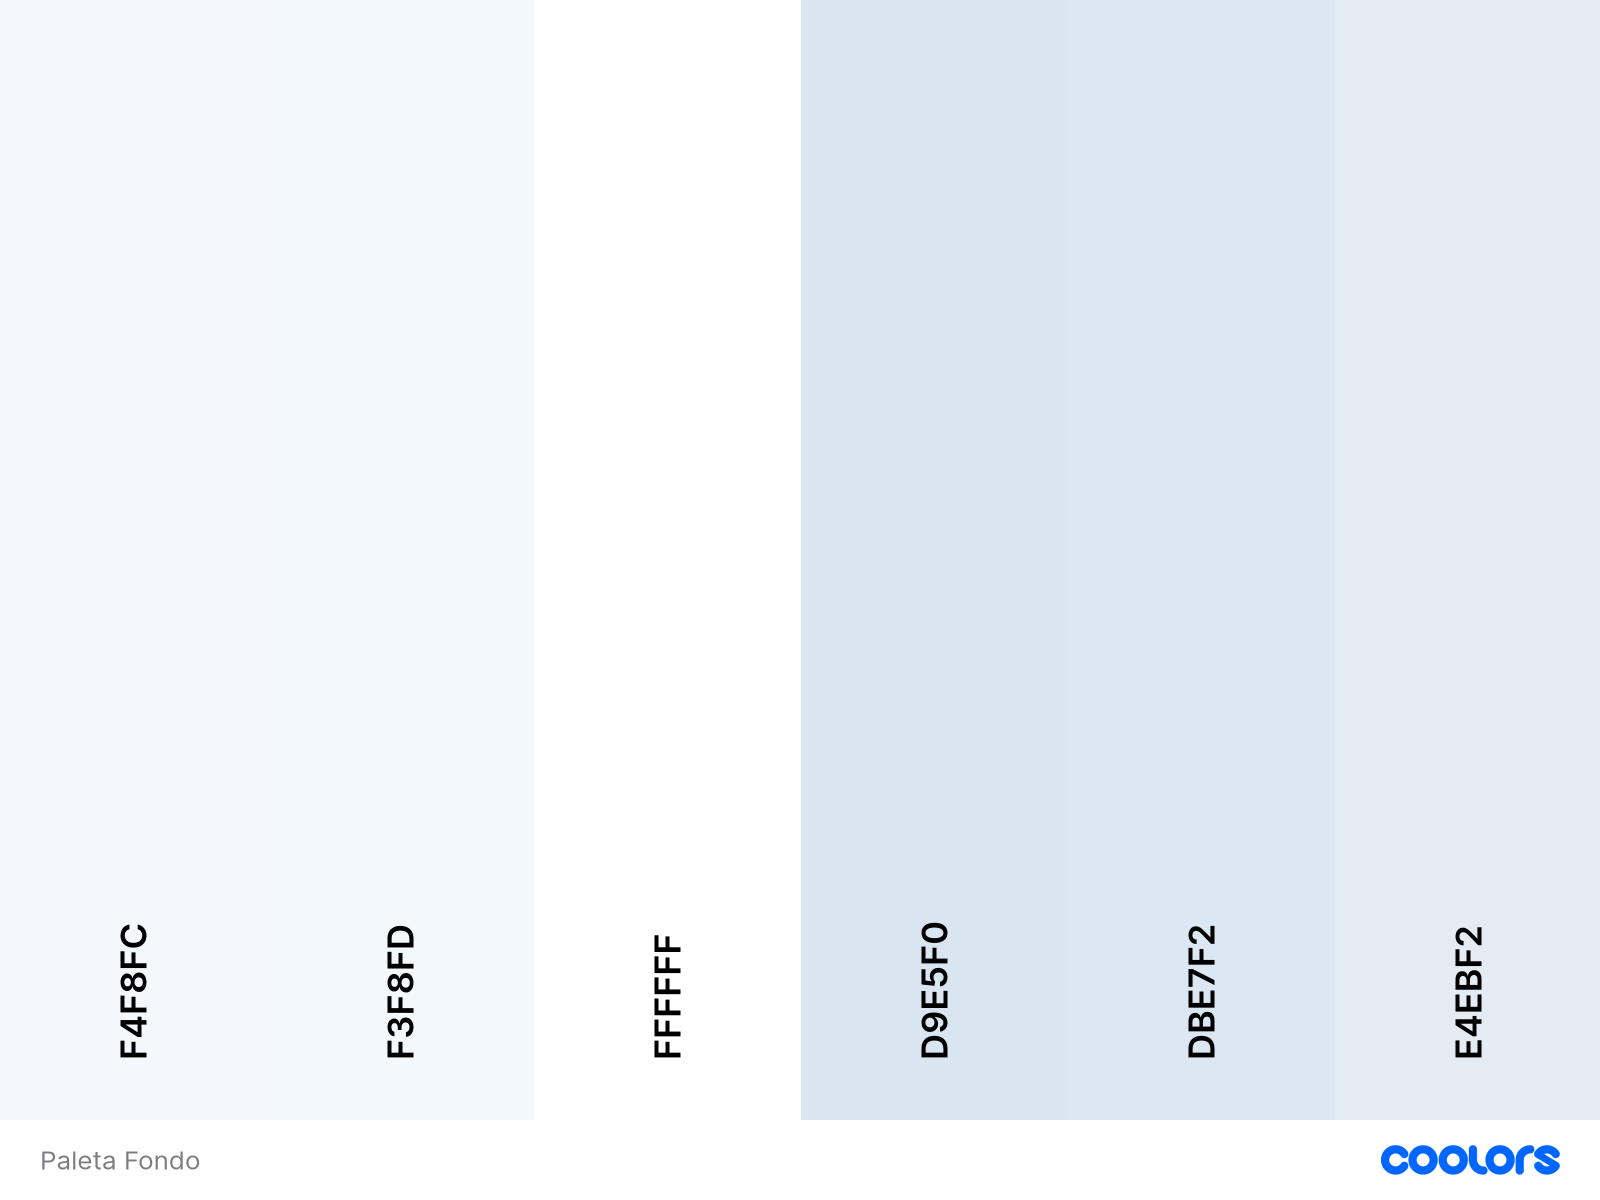
\includegraphics[width=0.8\linewidth]{figures/Paleta Fondo.png}
    \caption{Paleta de fondos.}
    \label{fig:paleta_fondo}
\end{figure}

Además, se definió una paleta específica para la pantalla del asistente conversacional, denominado \textit{Agente de oro}. En este caso se emplean tonos dorados con distintos niveles de contraste, con el fin de diferenciar visualmente esta funcionalidad del resto de la aplicación y reforzar su identidad propia dentro del sistema. La paleta correspondiente se recoge en la Figura~\ref{fig:paleta_agente}.

\begin{figure}[H]
    \centering
    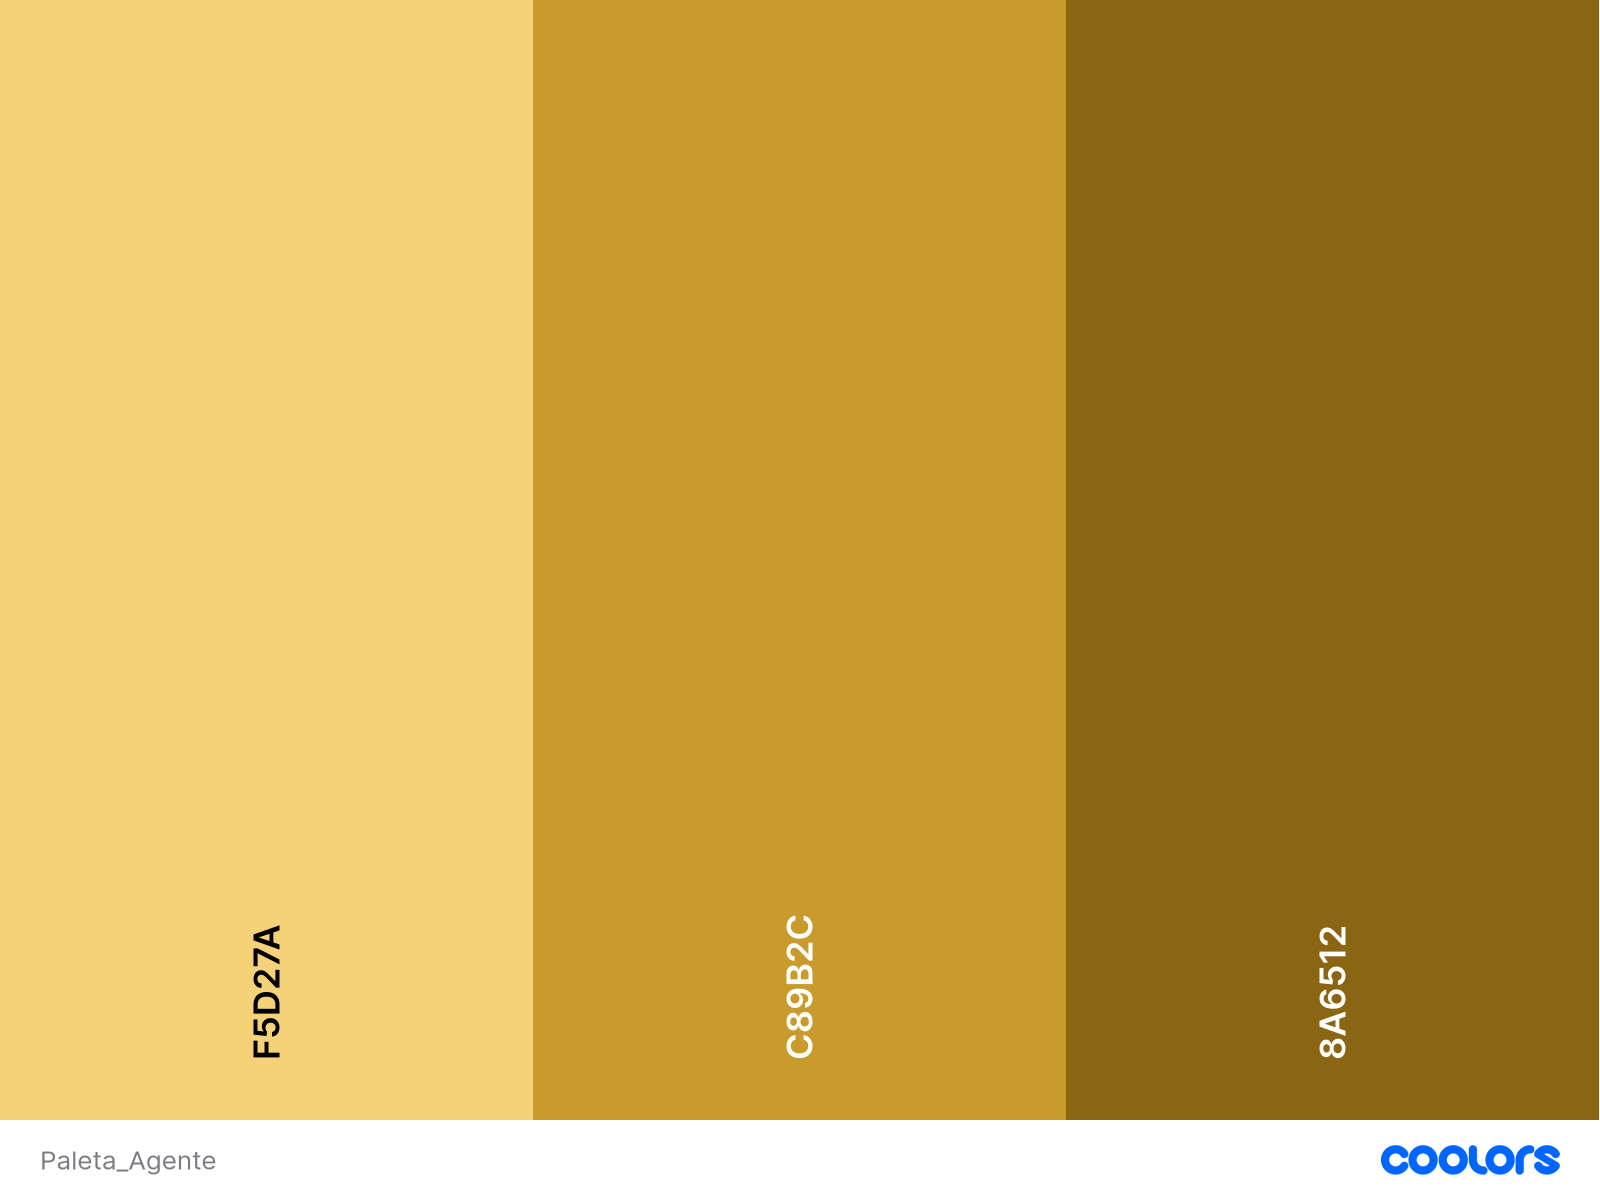
\includegraphics[width=0.8\linewidth]{figures/Paleta_Agente.png}
    \caption{Paleta de Agente de oro.}
    \label{fig:paleta_agente}
\end{figure}

Por último, para el modo oscuro se mantiene la misma línea visual basada en tonos azules, pero adaptada a fondos más oscuros. En este caso, los fondos de las pantallas y tarjetas emplean colores oscuros, mientras que los textos y elementos principales utilizan tonos claros para asegurar una correcta legibilidad. De esta forma, el modo oscuro conserva la identidad visual de la aplicación y ofrece una alternativa más cómoda en entornos con poca iluminación.

\newpage{\ }
\cleardoublepage

\chapter{Construcción del sistema}
\input{./sections/development/implementation}

\newpage{\ }
\cleardoublepage

\chapter{Minería de datos}
Este capítulo describe las técnicas de análisis implementadas en la aplicación, las variables utilizadas y los resultados que generan. Se distinguen dos grupos de procedimientos: por una parte, indicadores heurísticos construidos mediante agregaciones, reglas y ponderaciones definidas específicamente para el proyecto; por otra, modelos de aprendizaje automático y una simulación probabilística. Los scripts se encuentran en el directorio \path{DATA_MINING/SCRIPTS/} y sus salidas se almacenan en \path{DATA_MINING/DSA_DM/}.

\section{Métricas e indicadores estadísticos}

Los indicadores de este apartado no son modelos de aprendizaje automático. Se calculan mediante reglas deterministas que agregan, normalizan y ponderan las estadísticas disponibles. Su finalidad es resumir la información deportiva y facilitar su interpretación dentro de la aplicación.

\subsection{Índice de forma de un jugador}

El índice de forma de los jugadores se implementa en el script \path{estado_forma_jugador.py} y se calcula para la temporada 2025. El procedimiento parte de las estadísticas de cada futbolista por partido y construye primero una puntuación individual:

\begin{equation}
    S_{partido}=0.6\,N+0.4\,A,
\end{equation}

donde $N$ es la valoración del jugador proporcionada por la fuente de datos y $A$ representa una suma ponderada de sus acciones. Todos los jugadores reciben puntuación por goles y asistencias; además, se aplican contribuciones específicas según su posición. Por ejemplo, los defensas reciben puntuación por entradas e intercepciones y son penalizados por regates recibidos y goles concedidos, mientras que los porteros reciben puntuación por paradas y penaltis detenidos y son penalizados por los goles encajados.

La puntuación de la temporada se obtiene como la media de los encuentros en los que el jugador ha disputado al menos 15 minutos. Para calcular la forma reciente, se consideran sus siete apariciones más recientes y se conservan aquellas en las que ha jugado al menos 20 minutos. Si quedan menos de tres partidos válidos, el estado se clasifica como \textit{Pocos minutos}. En caso contrario, la evolución se define como:

\begin{equation}
    E=S_{reciente}-S_{temporada}.
\end{equation}

El jugador se clasifica con \textit{Rendimiento alto} cuando $E>0.3$, con \textit{Rendimiento bajo} cuando $E<-0.3$ y como \textit{Estable} en el resto de los casos. El resultado se almacena en \path{ESTADO_FORMA_JUGADORES_2025.csv}, junto con las puntuaciones de temporada y de forma reciente.

Este indicador permite detectar cambios recientes respecto al rendimiento medio del propio jugador. No constituye una valoración absoluta de su calidad ni una predicción de su rendimiento futuro.

\subsection{Índice de forma de un equipo}

El índice de forma de los equipos se implementa en \path{estado_forma_equipo.py}. Para cada equipo se seleccionan los cinco partidos más recientes y se asignan inicialmente 3 puntos por victoria, 1 por empate y 0 por derrota. Esta puntuación se ajusta utilizando los goles esperados del encuentro y la dificultad del rival. En particular, se añade un bono de 0.5 puntos cuando el rival pertenece a los seis primeros puestos de la clasificación tomada como referencia.

Los partidos más recientes reciben mayor importancia mediante una ponderación exponencial. Si los encuentros se ordenan del más antiguo al más reciente, sus pesos son $0.85^4$, $0.85^3$, $0.85^2$, $0.85$ y $1$. La media ponderada se normaliza posteriormente sobre una escala de 0 a 10:

\begin{equation}
    S_{equipo}=\min\left(10,\frac{10}{3}\frac{\sum_i w_i p_i}{\sum_i w_i}\right),
\end{equation}

donde $p_i$ es la puntuación ajustada de cada partido y $w_i$ su peso temporal. El estado se considera \textit{Positivo} cuando la nota es igual o superior a 5.5, \textit{Estable} cuando se encuentra entre 3.2 y 5.5, y \textit{Crítico} cuando es inferior a 3.2.

El script también almacena la media ponderada y la desviación estándar de las puntuaciones ponderadas en los campos \texttt{tendencia} y \texttt{variabilidad}, respectivamente. Estas medidas resumen el nivel reciente y su dispersión, pero no representan una tendencia temporal estimada mediante regresión.

\subsection{Análisis de necesidades de plantilla}

El script \path{aspectos_a_mejorar.py} identifica posibles posiciones que convendría reforzar. Para ello, agrega las estadísticas de los jugadores por equipo, temporada y posición, calcula tasas por 90 minutos y compara cada equipo con la media de la competición para esa misma temporada y posición.

Una métrica se considera baja cuando se encuentra al menos un 10\% por debajo de la media y alta cuando la supera, como mínimo, en un 10\%. Las reglas aplicadas se resumen en la Tabla~\ref{tab:criterios_necesidades}.

\begin{table}[H]
\centering
\caption{Criterios utilizados para detectar necesidades de plantilla.}
\label{tab:criterios_necesidades}
\begin{tabular}{|p{2.5cm}|p{4.7cm}|p{5.7cm}|}
\hline
\textbf{Necesidad} & \textbf{Indicadores analizados} & \textbf{Condición general} \\
\hline
Delantero & Goles a favor del equipo & Valor inferior a la media de la liga. \\
\hline
Extremo & Tasa de regates completados y asistencias por 90 minutos de los delanteros & Ambos valores inferiores a la media de la posición. \\
\hline
Medio ofensivo & Precisión de pase, pases clave y asistencias por 90 minutos de los mediocentros & Los tres valores inferiores a la media de la posición. \\
\hline
Pivote defensivo & Faltas, precisión de pase e intercepciones por 90 minutos de los mediocentros & Faltas superiores a la media y precisión e intercepciones inferiores. \\
\hline
Laterales & Asistencias y regates recibidos por 90 minutos de los defensas & Pocas asistencias y más regates recibidos que la media. \\
\hline
Central & Goles encajados, entradas, bloqueos e intercepciones por 90 minutos & Goles encajados superiores a la media y métricas defensivas inferiores. \\
\hline
Portero & Paradas y goles concedidos por 90 minutos & Menos paradas y más goles concedidos que la media. \\
\hline
\end{tabular}
\end{table}

Si no se cumple ninguna regla, el resultado indica que no existe una necesidad clara. Se trata de un sistema heurístico de apoyo: las asociaciones anteriores no demuestran por sí mismas que una posición sea la causa del rendimiento del equipo.

\subsection{Perfil estadístico de un jugador}

El script \path{ratings.py} transforma las estadísticas acumuladas de cada jugador en seis dimensiones: ataque, creación, defensa, portería, duelos y regates. Cada dimensión combina variables relacionadas con ese aspecto del juego. Por ejemplo, ataque utiliza goles y tiros a puerta; creación emplea pases, pases clave, asistencias y precisión; y defensa considera entradas, intercepciones, bloqueos y determinadas penalizaciones disciplinarias.

Para reducir el efecto de muestras pequeñas se aplica un factor de experiencia definido como:

\begin{equation}
    F_{experiencia}=\min\left(1,\frac{partidos}{10}\right).
\end{equation}

Las seis puntuaciones se calculan por jugador y temporada. Después se normalizan de forma independiente dentro de cada temporada, asignando el valor 10 al máximo observado en cada dimensión y escalando proporcionalmente el resto. También se calcula el percentil del jugador respecto a los demás futbolistas de esa campaña.

El resultado se guarda en \path{perfil_estadistico_jugadores.csv}. Estas puntuaciones son índices internos de la aplicación y no deben interpretarse como escalas universales o directamente comparables con valoraciones de otras fuentes.

\subsection{Recomendador de fichajes}

El recomendador se implementa en \path{recomendacion_fichajes_refuerzo.py}. Combina las necesidades de plantilla, los perfiles estadísticos, los grupos obtenidos mediante \textit{K-means}, las estadísticas por temporada, la clasificación de los equipos, la edad y el estado de forma reciente de los jugadores.

Primero se selecciona la temporada más reciente común a todas las fuentes y se consolidan las necesidades que corresponden a una misma posición general. Después se descartan los futbolistas con menos de 600 minutos y los que pertenecen al propio equipo. Los clubes se distribuyen en cuatro tramos según su posición: 1--3, 4--7, 8--14 y 15--20. Un club solo recibe candidatos procedentes de su mismo tramo o de uno inferior. También se excluyen cuatro parejas de clubes rivales definidas explícitamente en el script.

Para cada necesidad se identifica el clúster con mayor puntuación media en los atributos relevantes. Dentro de ese grupo se construye un perfil objetivo a partir del cuartil superior de jugadores. La similitud de cada candidato con dicho perfil se calcula mediante similitud coseno después de estandarizar las seis dimensiones estadísticas.

La puntuación final combina los siguientes factores:

\begin{itemize}
    \item Similitud con el perfil objetivo: 40\%;
    \item Nota media de la temporada: 25\%;
    \item Estado de forma reciente: 15\%;
    \item Edad: 10\%;
    \item Experiencia, medida mediante partidos disputados: 10\%.
\end{itemize}

La puntuación de edad alcanza su máximo en los 23,5 años, punto medio del intervalo ideal definido entre 20 y 27 años, y disminuye linealmente al alejarse de ese valor. Finalmente, se devuelven como máximo tres candidatos por necesidad. El resultado es determinista y explicable, pero no incorpora precio, duración del contrato, salario, lesiones ni disponibilidad real en el mercado; por tanto, debe entenderse como una recomendación estadística preliminar.

\subsection{Indicador de posibles goleadores}

El script \path{prob_goleadores.py} ordena a los jugadores de cada equipo según su propensión estimada a marcar en los partidos pendientes. Para cada futbolista, combina la media de goles de sus siete apariciones más recientes, su promedio goleador en la temporada 2025 y los goles anotados históricamente contra el rival:

\begin{equation}
    z=0.35\,G_{reciente}+0.45\,G_{temporada}+0.05\,\min(G_{rival},3).
\end{equation}

El valor se transforma mediante una función sigmoide, $p=1/(1+e^{-2(z-0.5)})$, y se limita a un máximo de 0.75. Para cada partido se seleccionan los tres jugadores con mayor valor de cada equipo.

Aunque el campo de salida se denomina \texttt{probabilidad}, el valor no ha sido calibrado contra frecuencias observadas. En consecuencia, debe interpretarse como un indicador heurístico para ordenar candidatos y no como una probabilidad estadística validada de marcar.

\section{Técnicas de minería de datos y aprendizaje automático}

\subsection{Jugadores similares mediante \textit{K-means}}

\textit{K-means} es una técnica de aprendizaje no supervisado que agrupa observaciones tratando de minimizar la distancia cuadrática respecto al centroide de su clúster \cite{azzami_clustering_2025}. En este proyecto se utiliza como primera etapa para reducir el conjunto de candidatos con perfiles estadísticos próximos.

\begin{figure}[H]
    \centering
    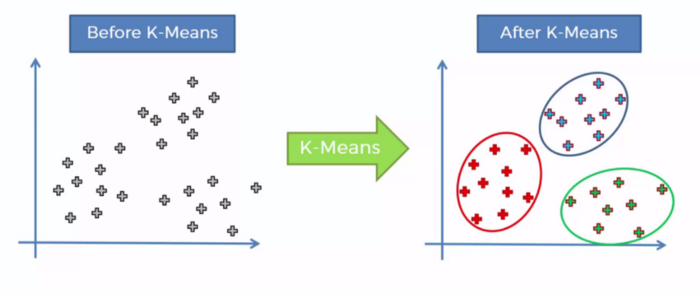
\includegraphics[width=0.7\linewidth]{figures/kmeans.png}
    \caption{Representación del funcionamiento de \textit{K-means}.}
    \label{fig:kmeans}
\end{figure}

\subsubsection{Implementación}

La implementación se encuentra en \path{similitud_jugadores.py} y utiliza como entrada \path{perfil_estadistico_jugadores.csv}. Las variables son ataque, creación, defensa, portería, duelos y regates. Los valores ausentes se sustituyen por la mediana y las variables se estandarizan mediante puntuaciones $z$ para evitar que su escala determine las distancias.

El proceso se ejecuta de forma independiente para cada temporada. El número de clústeres se calcula mediante $\lfloor\sqrt{n/2}\rfloor$, con un mínimo de 2 y un máximo de 20 cuando existen al menos tres jugadores. Se realizan cinco inicializaciones con semilla reproducible y se conserva la solución con menor inercia. Cada ejecución admite un máximo de 100 iteraciones.

Una vez asignados los clústeres, la similitud final se calcula mediante el coseno entre los perfiles estandarizados. Para cada jugador se buscan primero futbolistas de la misma posición y del mismo clúster. Si no existen cinco candidatos, la lista se completa con jugadores de la misma posición pertenecientes a otros clústeres. Por tanto, \textit{K-means} realiza la agrupación inicial, mientras que la similitud coseno determina el orden final de los cinco jugadores más parecidos.

\subsection{Predicción de partidos mediante clasificación supervisada}

El script \path{predicccion.py} plantea la predicción como un problema multiclase con tres resultados: victoria local, empate y victoria visitante. Se comparan Random Forest, Gradient Boosting y una máquina de vectores soporte (SVM) con núcleo RBF.

Para cada equipo se calculan, utilizando únicamente encuentros anteriores a la fecha del partido, las medias de puntos, goles a favor y goles en contra durante los últimos 5 y 10 partidos. También se obtienen las mismas variables restringidas a la condición de local o visitante. A estas características se añaden estadísticas acumuladas de temporada, como posición, puntos, diferencia de goles, victorias, empates, derrotas y resultados desglosados por localía.

Los partidos completados se ordenan cronológicamente. El 80\% inicial se utiliza para entrenamiento y el 20\% final para validación. Los valores ausentes se sustituyen por la mediana del conjunto de entrenamiento. En el caso de SVM, las variables se estandarizan antes de ajustar el modelo.

\subsubsection{Evaluación de los modelos}

Se emplean las métricas \textit{accuracy}, precisión macro, \textit{recall} macro y F1 macro. La F1 macro concede el mismo peso a las tres clases y resulta útil porque el empate suele estar peor representado que las victorias locales o visitantes.

\begin{table}[H]
\centering
\caption{Comparación de modelos para la predicción de partidos.}
\label{tab:evaluacion_prediccion}
\begin{tabular}{|l|c|c|c|c|}
\hline
\textbf{Modelo} & \textbf{Accuracy} & \textbf{Precisión macro} & \textbf{Recall macro} & \textbf{F1 macro} \\
\hline
SVM & 0.5586 & 0.5593 & 0.5527 & 0.5464 \\
\hline
Random forest & 0.5698 & 0.5464 & 0.5376 & 0.5385 \\
\hline
Gradient boosting & 0.5599 & 0.5446 & 0.5338 & 0.5311 \\
\hline
\end{tabular}
\end{table}

Random Forest obtiene la mayor tasa global de acierto, con un 56,98\%. Sin embargo, SVM alcanza la mejor F1 macro, con 0,5464, por lo que se utiliza para generar las predicciones de los partidos pendientes. El modelo se vuelve a entrenar con todos los partidos completados y produce las probabilidades de victoria local, empate y victoria visitante que consume posteriormente la simulación de Monte Carlo.

Las probabilidades proceden de la estimación interna habilitada por \texttt{SVC (probability=True)}. No se ha realizado una calibración externa adicional, por lo que deben interpretarse con cautela.

\subsection{Probabilidades de clasificación mediante simulación de Monte Carlo}

La simulación de Monte Carlo permite aproximar la distribución de resultados de un sistema mediante la repetición de escenarios aleatorios \cite{stock_physics-based_2022}. En este proyecto se utiliza para estimar la posición final de los equipos a partir de la clasificación actual y de las probabilidades 1X2 generadas por SVM.

El script \path{simulacion_montecarlo_laliga.py} ejecuta 10.000 simulaciones con semilla 42. En cada partido pendiente se genera un número aleatorio y se asigna una victoria local, un empate o una victoria visitante según las probabilidades correspondientes. A continuación se actualizan los puntos de ambos equipos.

Para aproximar el desempate, cada victoria simulada modifica la diferencia de goles $+1$ para el vencedor y $-1$ para el derrotado; los empates no la alteran. Si dos equipos continúan igualados a puntos y diferencia de goles, se ordenan por nombre. Esta simplificación permite generar una clasificación completa, aunque no reproduce todos los criterios oficiales de desempate ni simula marcadores exactos.

Al finalizar cada iteración se registran las siguientes categorías: campeón, puestos 1--4, puestos 5--7, puestos 8--17 y descenso, correspondiente a las posiciones 18--20. Las frecuencias obtenidas tras las 10.000 iteraciones se presentan como porcentajes estimados.

\subsection{Estimación de goles mediante regresión}

El script \path{prediccion_goles_partidos.py} complementa la predicción 1X2 estimando dos valores continuos: los goles del equipo local y los goles del visitante. Se emplean las mismas características recientes y acumuladas que en el modelo de clasificación.

Se comparan Random Forest Regressor, Gradient Boosting Regressor, Support Vector Regression y una red neuronal MLP. La evaluación utiliza la misma división temporal 80/20. Los valores predichos se limitan inferiormente a cero y se calculan el error absoluto medio (MAE), la raíz del error cuadrático medio (RMSE) y el coeficiente de determinación ($R^2$).

\begin{table}[H]
\centering
\caption{Comparación de modelos para la estimación de goles.}
\label{tab:evaluacion_goles_estimados}
\begin{tabular}{|l|c|c|c|}
\hline
\textbf{Modelo} & \textbf{MAE} & \textbf{RMSE} & \textbf{$R^2$} \\
\hline
Random Forest Regressor & 0.8237 & 1.0663 & 0.1791 \\
\hline
MLP Regressor & 0.8647 & 1.1016 & 0.1239 \\
\hline
SVR & 0.8844 & 1.1627 & 0.0240 \\
\hline
Gradient Boosting Regressor & 0.9063 & 1.1716 & 0.0091 \\
\hline
\end{tabular}
\end{table}

Random Forest Regressor obtiene el menor MAE y RMSE y el mayor$R^2$, por lo que se selecciona como modelo final. Un MAE de 0.8237 indica un error absoluto medio ligeramente inferior a un gol por equipo y partido. No obstante, el $R^2$ de 0.1791 muestra que el modelo explica una proporción reducida de la variabilidad de los marcadores.

La salida incluye los goles estimados de ambos equipos, su diferencia, un resultado 1X2 derivado y un marcador obtenido mediante redondeo. Estos valores no representan la métrica convencional de goles esperados o xG basada en la calidad de cada ocasión, sino una predicción agregada de goles a partir del historial de los equipos.

\section{Limitaciones metodológicas}

Los resultados presentados deben interpretarse dentro del alcance académico del proyecto. Los indicadores de forma, necesidades de plantilla, recomendación de fichajes y posibles goleadores se basan en reglas y ponderaciones diseñadas para la aplicación; no han sido validados mediante estudios con clubes, analistas o usuarios expertos.

Además, aunque las características recientes de los modelos predictivos se calculan utilizando partidos anteriores a cada encuentro, la implementación incorpora a todos los partidos de una temporada la última instantánea disponible de sus estadísticas acumuladas. En los encuentros históricos, esta instantánea puede contener información posterior a la fecha que se intenta predecir. Por ello, la división temporal reduce la mezcla cronológica entre entrenamiento y validación, pero no elimina por completo la posible fuga de información. Las métricas obtenidas deben considerarse una evaluación preliminar y no una estimación definitiva del rendimiento ante datos futuros.

Por último, los modelos dependen de la cobertura y calidad de API-Football y no incorporan variables potencialmente relevantes como lesiones, sanciones, alineaciones confirmadas, cambios de entrenador o descanso entre encuentros. Estas limitaciones no impiden su uso como demostración funcional, pero sí desaconsejan interpretar los resultados como pronósticos profesionales.


\newpage{\ }
\cleardoublepage

\chapter{Pruebas del sistema}
% ------------------------------------------------------------------------------
% Este fichero es parte de la plantilla LaTeX para la realización de Proyectos
% Final de Grado, protegido bajo los términos de la licencia GFDL.
% Para más información, la licencia completa viene incluida en el
% fichero fdl-1.3.tex

% Copyright (C) 2012 SPI-FM. Universidad de Cádiz
% ------------------------------------------------------------------------------

En este capítulo se presenta el plan de pruebas del sistema de información, incluyendo los diferentes tipos de pruebas que se han llevado a cabo, ya sean manuales (mediante listas de comprobación) o automatizadas mediante algún \textit{software} específico de pruebas.

\section{Estrategia}

La validación se realizó de forma incremental mediante pruebas unitarias, de
integración y de sistema. Se comprobaron las funcionalidades principales y la
comunicación entre el \textit{frontend}, el \textit{backend}, la base de datos y
los servicios externos. Las tablas recogen los casos más representativos, que se
consideraron superados cuando el resultado obtenido coincidió con el esperado.

Tras cada corrección se repitió la prueba afectada y los flujos principales de
acceso, consulta y gestión de datos, con el fin de detectar posibles regresiones.
Las pruebas fueron ejecutadas por el autor en un entorno local, utilizando
Docker para el \textit{backend} y PostgreSQL, y Expo Go en un dispositivo Android
para la aplicación móvil.

\section{Pruebas Unitarias}

Las pruebas unitarias tienen por objetivo localizar errores en cada nuevo artefacto \textit{software} desarrollado, antes de que se produzca la integración con el resto de artefactos del sistema.

En este proyecto, las pruebas unitarias se han centrado principalmente en aquellos módulos que contienen lógica propia de la aplicación, como la autenticación de usuarios, la validación de datos, la gestión de favoritos, el tratamiento de respuestas del backend y determinadas funciones auxiliares utilizadas por la interfaz. No se han considerado dentro de este apartado los procesos internos de extracción o generación de resultados analíticos, ya que el plan de pruebas se orienta principalmente a la validación de la aplicación final.

Las pruebas se han realizado de forma manual y mediante comprobaciones controladas sobre funciones concretas, verificando que cada módulo devuelve el resultado esperado ante entradas válidas, entradas incorrectas y situaciones límite.

\begin{table}[H]
\centering
\caption{Pruebas unitarias realizadas}
\label{tab:pruebas_unitarias}
\renewcommand{\arraystretch}{1.2}
\begin{tabular}{|l|p{3cm}|p{5cm}|p{4cm}|}
\hline
\textbf{Código} & \textbf{Módulo} & \textbf{Prueba realizada} & \textbf{Resultado esperado} \\ \hline

PU-01 & Autenticación & Iniciar sesión con credenciales válidas. & El sistema devuelve los datos del usuario y permite acceder a la aplicación. \\ \hline

PU-02 & Autenticación & Iniciar sesión con una contraseña incorrecta. & El sistema rechaza el acceso y muestra un mensaje de error. \\ \hline

PU-03 & Registro & Crear una cuenta con datos válidos. & La cuenta se registra correctamente. \\ \hline

PU-04 & Registro & Crear una cuenta con un correo ya existente. & El sistema informa de que el correo ya está registrado. \\ \hline

PU-05 & Validación de formularios & Enviar formularios con campos obligatorios vacíos. & El sistema solicita completar los campos necesarios. \\ \hline

PU-06 & Favoritos & Añadir un equipo o jugador a favoritos. & El elemento queda marcado como favorito. \\ \hline

PU-07 & Favoritos & Eliminar un equipo o jugador de favoritos. & El elemento deja de aparecer como favorito. \\ \hline

PU-08 & Buscador & Introducir un texto parcial de búsqueda. & El sistema devuelve coincidencias relacionadas con equipos o jugadores. \\ \hline

PU-09 & Chatbot & Enviar una pregunta vacía. & La consulta no se envía y se mantiene la interfaz sin cambios. \\ \hline

PU-10 & Chatbot & Enviar una consulta fuera del dominio futbolístico. & El asistente informa de que no puede responder de forma fiable. \\ \hline

PU-11 & Gestión de sesión & Cerrar sesión desde la aplicación. & Se eliminan los datos locales de sesión y se vuelve a la pantalla de inicio. \\ \hline

PU-12 & Tratamiento de errores & Simular una respuesta incorrecta del backend. & La pantalla muestra un mensaje de error adecuado. \\ \hline

\end{tabular}
\end{table}

Estas pruebas permitieron comprobar el comportamiento básico de los módulos principales antes de validar su funcionamiento conjunto mediante las pruebas de integración. En aquellos casos en los que se detectaron errores, se corrigieron antes de continuar con la integración de las pantallas y servicios afectados.

\section{Pruebas de integración}

Las pruebas de integración permiten comprobar que los distintos componentes del
sistema se comunican correctamente. A diferencia de las pruebas unitarias, estas
pruebas no analizan cada módulo de manera aislada, sino el intercambio de
información entre ellos.

Para realizar las pruebas se utilizó un conjunto de datos conocido previamente.
Cada caso de prueba contiene una acción, un resultado esperado, el resultado
obtenido y una evidencia de su ejecución. Se probaron tanto situaciones correctas
como algunos errores representativos.

\subsection{\textit{Backend} -- Base de datos}

Estas pruebas comprueban que el \textit{backend} puede conectarse a PostgreSQL,
consultar la información almacenada y realizar correctamente las operaciones de
persistencia necesarias.

\begin{table}[H]
    \centering
    \small
    \begin{tabularx}{\textwidth}{|l|X|X|c|}
        \hline
        \textbf{ID} & \textbf{Prueba} & \textbf{Resultado esperado} &
        \textbf{Estado} \\ \hline

        PI-BD-01 &
        Solicitar mediante un \textit{endpoint} la información de un equipo,
        jugador o partido existente. &
        El servidor devuelve un código HTTP 200 y los datos coinciden con los
        almacenados en PostgreSQL. &
        Superada \\ \hline

        PI-BD-02 &
        Realizar una operación de almacenamiento disponible en la aplicación,
        como registrar un usuario o guardar una preferencia. &
        La operación devuelve una respuesta satisfactoria y el nuevo registro
        aparece correctamente en la base de datos. &
        Superada \\ \hline

        PI-BD-03 &
        Solicitar un recurso cuyo identificador no existe. &
        El servidor devuelve un código de error controlado, como HTTP 404, sin
        producir cambios en la base de datos. &
        Superada \\ \hline
    \end{tabularx}
    \caption{Pruebas de integración entre el \textit{backend} y la base de datos}
    \label{tab:pruebas-backend-bd}
\end{table}

La primera prueba puede verificarse comparando la respuesta obtenida mediante
Postman con el resultado de una consulta SQL ejecutada directamente sobre la
base de datos. En las operaciones de escritura, se comprueba también que el
registro haya sido almacenado y que no se hayan modificado otros datos.

% Insertar aquí una captura de Postman y, si se considera necesario,
% otra captura con la consulta realizada en PostgreSQL.
\subsection{\textit{Frontend} -- \textit{Backend}}

El objetivo de estas pruebas es comprobar que la aplicación móvil envía
correctamente las peticiones al \textit{backend}, interpreta sus respuestas y
muestra al usuario la información recibida.

\begin{table}[H]
    \centering
    \small
    \begin{tabularx}{\textwidth}{|l|X|X|c|}
        \hline
        \textbf{ID} & \textbf{Prueba} & \textbf{Resultado esperado} &
        \textbf{Estado} \\ \hline

        PI-FB-01 &
        Acceder desde la aplicación a una pantalla que muestre equipos,
        jugadores, partidos o estadísticas. &
        El \textit{frontend} realiza la petición y muestra los mismos datos que
        devuelve el \textit{backend}. &
        Superada \\ \hline

        PI-FB-02 &
        Enviar un formulario desde la aplicación, como el inicio de sesión o el
        registro de un usuario. &
        Los datos llegan al servidor y la aplicación procesa correctamente la
        respuesta recibida. &
        Superada \\ \hline

        PI-FB-03 &
        Introducir datos incorrectos en un formulario o provocar una respuesta
        de error del servidor. &
        La aplicación no se bloquea y muestra al usuario un mensaje de error
        comprensible. &
        Superada \\ \hline

        PI-FB-04 &
        Intentar realizar una consulta con el \textit{backend} detenido o sin
        conexión de red. &
        La aplicación controla el fallo de conexión y permite volver a intentar
        la operación. &
        Superada \\ \hline
    \end{tabularx}
    \caption{Pruebas de integración entre el \textit{frontend} y el
    \textit{backend}}
    \label{tab:pruebas-frontend-backend}
\end{table}

Para verificar estas pruebas se comparan los datos mostrados en la interfaz con
la respuesta del \textit{endpoint} correspondiente. Como evidencia se pueden
incluir capturas de la aplicación y de la respuesta obtenida mediante Postman.

\subsection{Chatbot -- \textit{Backend} -- Base de datos}

Estas pruebas validan el flujo completo de una consulta realizada al
chatbot. El mensaje introducido por el usuario debe enviarse al
\textit{backend}, procesarse y generar una consulta de lectura sobre la base de
datos. Finalmente, la respuesta debe regresar hasta la interfaz de la aplicación.

Debido a que el modelo puede generar respuestas con redacciones diferentes, no
se compara el texto de forma literal. La validación se realiza comprobando que
los datos relevantes de la respuesta coincidan con los almacenados en la base
de datos.

\begin{table}[H]
    \centering
    \small
    \begin{tabularx}{\textwidth}{|l|X|X|c|}
        \hline
        \textbf{ID} & \textbf{Prueba} & \textbf{Resultado esperado} &
        \textbf{Estado} \\ \hline

        PI-CB-01 &
        Formular una pregunta sobre un dato conocido, como la clasificación de
        un equipo o los goles marcados por un jugador en una temporada. &
        El chatbot devuelve una respuesta cuyo dato principal coincide
        con la información almacenada en PostgreSQL. &
        Superada \\ \hline

        PI-CB-02 &
        Realizar una consulta sobre información inexistente o que no se
        encuentre almacenada. &
        El sistema informa de que no dispone de la información y no genera un
        dato como si fuera verdadero. &
        Superada \\ \hline

        PI-CB-03 &
        Introducir una petición que intente modificar o eliminar información de
        la base de datos. &
        La operación es rechazada y la base de datos permanece sin cambios. &
        Superada \\ \hline

        PI-CB-04 &
        Enviar una pregunta vacía, incompleta o no relacionada con la información
        que puede consultar el sistema. &
        El sistema controla la entrada y devuelve un mensaje adecuado sin
        producir un error interno. &
        Superada \\ \hline
    \end{tabularx}
    \caption{Pruebas de integración del chatbot}
    \label{tab:pruebas-chatbot}
\end{table}

Para comprobar la exactitud de la primera prueba, se consulta directamente la
base de datos y se compara el resultado con la información proporcionada por el
chatbot. En la prueba de seguridad se registra el estado de la base de
datos antes y después de la petición, verificando que no se haya producido
ninguna modificación.
\section{Pruebas de Sistema}
En esta actividad se realizan las pruebas de sistema de modo que se asegure que el sistema cumple con todos los requisitos establecidos: funcionales, de almacenamiento, reglas de negocio y no funcionales. Se suelen desarrollar en un entorno específico para pruebas.

\subsection{Pruebas funcionales}

Las pruebas funcionales verifican de extremo a extremo los principales casos de
uso del sistema. Para evitar repeticiones, se agrupan las operaciones que forman
parte de un mismo flujo.

\begin{table}[H]
    \centering
    \small
    \begin{tabularx}{\textwidth}{|l|p{3cm}|X|c|}
        \hline
        \textbf{ID} & \textbf{Funcionalidad} & \textbf{Comprobación} &
        \textbf{Estado} \\ \hline

        PF-01 & Acceso a la aplicación &
        Registrar una cuenta, iniciar sesión con ella y cerrar la sesión. &
        Superada \\ \hline

        PF-02 & Consulta deportiva &
        Consultar temporadas, equipos, jugadores y partidos mediante listados,
        filtros y pantallas de detalle. &
        Superada \\ \hline

        PF-03 & Favoritos &
        Añadir y eliminar equipos o jugadores de la selección personal. &
        Superada \\ \hline

        PF-04 & Análisis avanzados &
        Seleccionar una temporada y consultar los análisis de favoritos,
        equipos, jugadores y predicciones. &
        Superada \\ \hline

        PF-05 & Chatbot &
        Realizar una consulta futbolística y comprobar que la respuesta utiliza
        los datos disponibles en el sistema. &
        Superada \\ \hline

        PF-06 & Simulador &
        Introducir resultados, recalcular la clasificación y consultar las
        probabilidades obtenidas mediante simulación. &
        Superada \\ \hline

        PF-07 & Gestión del perfil &
        Consultar y modificar el perfil, y cambiar la contraseña verificando la
        actual. &
        Superada \\ \hline

        PF-08 & Eliminación de cuenta &
        Confirmar la eliminación y comprobar que las credenciales dejan de
        permitir el acceso. &
        Superada \\ \hline
    \end{tabularx}
    \caption{Pruebas funcionales del sistema}
    \label{tab:pruebas-funcionales}
\end{table}

Todas las pruebas finalizaron con el resultado esperado, incluidos los mensajes
mostrados ante datos incorrectos o incompletos.

\subsection{Pruebas no funcionales}

Las pruebas no funcionales tienen como objetivo evaluar el comportamiento general del sistema en relación con los atributos de calidad definidos en los requisitos no funcionales. Para ello, se comprueban aspectos como el rendimiento, la compatibilidad, la usabilidad, la fiabilidad, la seguridad, la mantenibilidad y la portabilidad de la aplicación.

A continuación, se describen las pruebas planteadas para validar cada uno de estos requisitos:

\begin{itemize}

    \item PNF1. Adecuación funcional (RNF1): se comprueba que las funcionalidades disponibles cubren las necesidades principales del usuario. Para ello, se recorren los distintos módulos de la aplicación, verificando el acceso a los datos y estadísticas futbolísticas, la consulta de información, la interacción con el chatbot y la gestión de las funcionalidades asociadas al usuario. La prueba se considera satisfactoria si todas las acciones previstas pueden completarse correctamente.

    \item PNF2. Eficiencia de desempeño (RNF2): se miden los tiempos de respuesta de las principales operaciones del sistema, como la carga de estadísticas, la consulta de información almacenada en PostgreSQL y la generación de respuestas por parte del chatbot. Las consultas se ejecutan varias veces en condiciones normales de uso para comprobar que los tiempos se mantienen estables y que la interfaz no queda bloqueada durante su procesamiento.

    \item PNF3. Compatibilidad (RNF3): se verifica la comunicación entre los distintos componentes tecnológicos del sistema. Esto incluye la conexión del \textit{backend} con PostgreSQL, la obtención de información desde API Football, la comunicación con la API de Gemini y el intercambio de datos entre el \textit{frontend} desarrollado con React Native y el servidor. La prueba se supera cuando los componentes intercambian información correctamente y los datos recibidos pueden ser procesados por la aplicación.

    \item PNF4. Usabilidad (RNF4): se realizan recorridos por las principales pantallas de la aplicación, comprobando que los elementos de navegación sean visibles, que los textos y botones resulten comprensibles y que exista coherencia visual entre las distintas vistas. También se comprueba que las acciones habituales puedan realizarse sin conocimientos técnicos ni instrucciones adicionales.

    \item PNF5. Fiabilidad (RNF5): se simulan situaciones de error, como la pérdida de conexión con el servidor, la indisponibilidad temporal de un servicio externo, la recepción de respuestas inválidas o la introducción de consultas incorrectas. El sistema debe controlar estas situaciones sin cerrarse inesperadamente y mostrar al usuario un mensaje de error comprensible, permitiéndole continuar utilizando la aplicación o volver a intentar la operación.

    \item PNF6. Seguridad (RNF6): se comprueba que un usuario no autenticado no pueda acceder a información personal ni a funcionalidades restringidas. Asimismo, se verifica que las contraseñas no se almacenen en texto plano y que las credenciales incorrectas sean rechazadas. En el caso del chatbot, se realizan consultas que intentan modificar o eliminar información de la base de datos, comprobando que únicamente se permitan operaciones de lectura autorizadas.

    \item PNF7. Mantenibilidad (RNF7): se revisa la estructura del proyecto para comprobar que existe una separación clara entre el \textit{frontend}, el \textit{backend}, el proceso ETL, los modelos de minería de datos y la base de datos. También se verifica que los componentes presenten responsabilidades diferenciadas y puedan modificarse sin afectar innecesariamente al resto del sistema.

    \item PNF8. Portabilidad (RNF8): se ejecuta la aplicación en diferentes dispositivos o emuladores Android compatibles con React Native y Expo, comprobando que las pantallas se adapten a distintas resoluciones. Además, se realiza el despliegue del sistema mediante Docker en un entorno limpio, verificando que los servicios puedan iniciarse a partir de la configuración proporcionada sin requerir modificaciones específicas en el código.

\end{itemize}

La superación de estas pruebas permite comprobar que el sistema no solo implementa las funcionalidades previstas, sino que también presenta un comportamiento adecuado en términos de calidad, rendimiento, seguridad y facilidad de mantenimiento. De esta forma, se valida el cumplimiento de los requisitos no funcionales definidos conforme a las características establecidas por el estándar ISO/IEC 25010.


% \newpage{\ }
% \cleardoublepage

% \chapter{Despliegue del Sistema}
% Este capítulo recoge la arquitectura física planteada para el sistema, las instrucciones para su despliegue y las instrucciones para la operación y mantenimiento del nivel de servicio.

\section{Arquitectura Física}
En este apartado, describimos los principales elementos \textit{hardware} que forman la arquitectura física de nuestro sistema. Se debe incluir un modelo de despliegue en el cual se describe cómo los elementos \textit{software} son instalados y ejecutados en los elementos \textit{hardware} (físicos o virtuales). También se incluyen las especificaciones y los requisitos del \textit{hardware} (servidores, etc.), así como de los elementos \textit{software} (sistemas operativos, servicios, aplicaciones, etc.) necesarios.

\section{Instrucciones de despliegue}
A continuación, se describen las instrucciones de instalación del sistema sobre la infraestructura física descrita anteriormente.

\subsection{Requisitos previos}
Requisitos de hardware y \textit{software} para la correcta instalación del sistema.

\subsection{Inventario de componentes}
Lista de los componentes hardware y software que se incluyen en la versión del producto.

\subsection{Procedimientos de instalación}
Procedimientos de instalación y configuración de cada componente hardware y software (base y desarrollado) para asegurar la correcta instalación y explotación del sistema, así como aquellos procedimientos necesarios de migración/carga de datos.

\subsection{Pruebas de implantación}
Descripción de las pruebas a realizar después de la instalación del sistema. 

\section{Instrucciones para la operación del sistema y mantenimiento del nivel de servicio}
Procedimientos necesarios para asegurar el correcto funcionamiento, rendimiento, disponibilidad y seguridad del sistema: back-ups, chequeo de logs, etc. También es preciso indicar claramente aquellas actuaciones precisas necesarias para el mantenimiento preventivo del sistema y así prevenir posibles fallos en el mismo. 
 
    % EPILOGO
    \part{Epílogo}
    \null\vfill


% Conclusiones
\chapter{Conclusiones}
\label{cap:conclusiones}
En este último capítulo se detallan las lecciones aprendidas tras el desarrollo del presente proyecto y se identifican las posibles oportunidades de mejora sobre el \textit{software} desarrollado.

\section{Objetivos alcanzados}

El objetivo principal de este Trabajo Fin de Grado era desarrollar una aplicación móvil multiplataforma que permitiese consultar, visualizar y analizar información futbolística mediante técnicas de inteligencia de negocio, minería de datos y aprendizaje automático. Para ello, se planteó una solución que integrase datos históricos de LaLiga, una arquitectura de almacenamiento orientada al análisis, una API de consulta, una interfaz móvil y una capa de análisis avanzado.

En primer lugar, se ha conseguido construir una base de datos estructurada a partir de información histórica de la Primera División Española. Para ello, se ha desarrollado un proceso de extracción, transformación y carga de datos que permite pasar de información procedente de una API externa a un modelo físico organizado y preparado para su explotación. Este proceso ha permitido disponer de datos relacionados con temporadas, equipos, jugadores, partidos, eventos y estadísticas de rendimiento.

También se ha alcanzado el objetivo de diseñar una arquitectura de inteligencia de negocio basada en un modelo de datos orientado al análisis. La base de datos se ha organizado mediante un esquema en constelación, formado por tablas de dimensiones y tablas de hechos, lo que facilita la consulta de información desde diferentes perspectivas. Gracias a esta estructura, la aplicación puede mostrar datos a nivel de temporada, equipo, jugador y partido de forma ordenada y coherente.

Otro de los objetivos alcanzados ha sido la implementación de una API REST que actúa como capa intermedia entre la aplicación móvil y la base de datos. Esta API permite separar la lógica de acceso a datos de la capa visual, facilitando la consulta de información desde las distintas pantallas de la aplicación. A través de ella se obtienen listados, detalles, rankings, gráficos, favoritos, predicciones y respuestas asociadas al asistente conversacional.

En cuanto a la aplicación móvil, se ha desarrollado una interfaz que permite navegar entre las secciones principales del sistema: inicio, temporadas, equipos, jugadores, partidos, favoritos, perfil, simulación, análisis mediante \textit{data mining} y asistente inteligente. Las pantallas de detalle y los dashboards permiten representar la información de manera visual e interactiva, evitando que el usuario tenga que interpretar directamente tablas extensas o datos sin procesar.

Además de la consulta estadística tradicional, se han incorporado resultados generados mediante técnicas de minería de datos y aprendizaje automático. Entre ellos se incluyen predicciones de partidos, simulaciones de clasificación, estados de forma de equipos y jugadores, jugadores similares, probables goleadores y recomendaciones de fichajes. Estos resultados se han centralizado en una pantalla específica de \textit{data mining}, dando mayor protagonismo a la parte analítica del proyecto.

Por último, se ha integrado un asistente conversacional basado en inteligencia artificial, denominado Agente de Oro. Esta funcionalidad permite al usuario realizar preguntas en lenguaje natural sobre la información almacenada en el sistema, facilitando el acceso a datos concretos sin necesidad de recorrer manualmente todas las pantallas de la aplicación.

En conjunto, puede afirmarse que el proyecto ha cumplido con su objetivo general: desarrollar una aplicación móvil capaz de acercar el análisis avanzado de datos futbolísticos a usuarios no necesariamente especializados, combinando visualización, predicción, simulación y consulta inteligente dentro de una misma plataforma.

\section{Lecciones aprendidas}

El desarrollo del proyecto ha permitido extraer varias conclusiones relevantes tanto desde el punto de vista técnico como desde el punto de vista funcional.

Una de las principales lecciones aprendidas es la importancia de contar con una estructura de datos sólida antes de desarrollar las funcionalidades visibles de la aplicación. En un proyecto basado en análisis deportivo, la calidad de los resultados depende directamente de la calidad, coherencia y organización de los datos disponibles. Por este motivo, el diseño del modelo de datos y el proceso de transformación han sido elementos fundamentales para que posteriormente pudieran construirse dashboards, rankings y modelos predictivos.

También se ha comprobado que la visualización de datos es tan importante como el propio cálculo de las métricas. Muchos indicadores deportivos pueden resultar complejos si se presentan únicamente en forma de tablas o valores numéricos. Sin embargo, al representarlos mediante tarjetas, gráficos, rankings y dashboards, la información resulta mucho más comprensible para el usuario. Esta idea ha sido especialmente relevante en las pantallas de temporada, equipo, jugador, partido y \textit{data mining}.

Otra lección importante es que los modelos de minería de datos aportan valor cuando sus resultados se integran de forma clara dentro de la aplicación. No basta con calcular predicciones, simulaciones o agrupaciones de jugadores; es necesario presentarlas de una manera que el usuario pueda entender e interpretar. Por ello, la creación de una pantalla específica de \textit{data mining} ha permitido dar mayor visibilidad a estos resultados y diferenciarlos de la consulta estadística tradicional.

El desarrollo también ha puesto de manifiesto la utilidad de separar correctamente las distintas capas del sistema. La división entre aplicación móvil, backend, base de datos y procesos analíticos facilita el mantenimiento del proyecto y permite modificar una parte del sistema sin afectar directamente al resto. Esta separación ha sido especialmente útil al añadir nuevas funcionalidades, como favoritos, simulaciones, predicciones o el asistente conversacional.

En relación con el asistente inteligente, se ha observado que el uso de lenguaje natural puede mejorar la experiencia de usuario, especialmente cuando se desea consultar información concreta. No obstante, también se ha comprobado que esta funcionalidad requiere restricciones claras para evitar consultas incorrectas, ambiguas o fuera del dominio del sistema. Por ello, ha sido necesario limitar su uso a consultas relacionadas con la información futbolística almacenada y controlar que las operaciones generadas sean seguras.

Por último, el proyecto ha servido para comprender que una aplicación de análisis deportivo no debe centrarse únicamente en acumular funcionalidades, sino en organizar la información de forma útil. La prioridad debe ser que el usuario pueda encontrar rápidamente lo que busca, interpretar los resultados y entender el valor de los datos mostrados.

\section{Trabajo futuro}

Aunque el proyecto ha alcanzado los objetivos planteados, existen diferentes líneas de trabajo futuro que permitirían ampliar sus capacidades y acercarlo a un entorno de uso real.

Una primera mejora sería ampliar la cobertura de datos. Actualmente, el sistema se centra en la Primera División Española, por lo que una evolución natural consistiría en incorporar otras competiciones, como Segunda División, competiciones europeas o ligas extranjeras. Esto permitiría comparar equipos y jugadores entre distintos contextos y enriquecer los análisis disponibles.

Otra línea de mejora sería incorporar datos en tiempo real. En el estado actual del proyecto, la aplicación trabaja principalmente con datos históricos y datos previamente cargados. En un entorno de producción, sería interesante integrar servicios que proporcionen información en directo sobre partidos, eventos, alineaciones, lesiones o estadísticas actualizadas durante el encuentro. Esto permitiría ofrecer predicciones y análisis más dinámicos.

También sería posible mejorar los modelos de predicción mediante la incorporación de nuevas variables. Por ejemplo, podrían añadirse datos sobre lesiones, sanciones, alineaciones probables, calendario acumulado, descanso entre partidos, mercado de fichajes o métricas avanzadas como xG y xA cuando estuvieran disponibles. Estos factores podrían aumentar la precisión de los modelos y aportar una visión más completa del rendimiento deportivo.

En relación con la simulación de temporada, una posible mejora consistiría en permitir al usuario crear y guardar múltiples escenarios personalizados. De esta forma, podría comparar distintas hipótesis sobre resultados futuros y analizar cómo afectarían a la clasificación final, a la lucha por el título, a la clasificación europea o al descenso.

La pantalla de \textit{data mining} también podría evolucionar hacia una sección más personalizada. Actualmente centraliza los resultados analíticos del sistema, pero en futuras versiones podría priorizar automáticamente la información relacionada con los equipos y jugadores favoritos del usuario. Esto permitiría ofrecer una experiencia más adaptada a los intereses de cada persona.

Otra línea de trabajo relevante sería mejorar el asistente conversacional. En futuras versiones, el sistema podría ser capaz de interpretar preguntas más complejas, explicar gráficos, comparar jugadores o equipos y generar resúmenes automáticos de partidos, temporadas o trayectorias. También sería interesante mejorar el control de las consultas generadas para aumentar la seguridad y fiabilidad de las respuestas.

Desde el punto de vista de despliegue, el proyecto podría evolucionar hacia una versión en producción. Para ello sería necesario alojar el backend y la base de datos en un servidor externo, configurar un dominio, establecer copias de seguridad, monitorizar el sistema y valorar la publicación de la aplicación en tiendas móviles. Además, habría que considerar el coste recurrente de servicios externos, como APIs deportivas o modelos de inteligencia artificial.

Finalmente, sería recomendable realizar pruebas con usuarios reales. Aunque durante el desarrollo se han realizado pruebas funcionales y de integración, una validación con aficionados, analistas deportivos o perfiles técnicos permitiría obtener información más precisa sobre la utilidad de la aplicación, la claridad de los dashboards, la comprensión de las predicciones y la facilidad de uso del asistente conversacional.

En definitiva, el trabajo realizado constituye una base funcional sobre la que pueden desarrollarse nuevas mejoras. La aplicación demuestra que es posible integrar datos deportivos, visualización, modelos predictivos y consultas inteligentes en una herramienta móvil accesible, quedando abiertas varias líneas de evolución hacia un sistema más completo, personalizado y cercano a un uso profesional.

\newpage{\ }
\cleardoublepage

% Licencia
\chapter*{\rlap{Información sobre Licencia}}
\label{cap:licencia}
\phantomsection
\addcontentsline{toc}{chapter}{Información sobre Licencia}
La documentación del presente Trabajo Fin de Grado se distribuye bajo la licencia \href{https://creativecommons.org/licenses/by/4.0/}{Creative Commons Atribución/Reconocimiento 4.0 Internacional}.

El \textit{software} desarrollado en este proyecto se proporciona con fines académicos y de investigación. Su uso, modificación o reutilización deberá respetar la autoría del trabajo y las condiciones establecidas por la Universidad de Cádiz para los Trabajos Fin de Grado.

Los datos utilizados en la aplicación proceden de fuentes externas, por lo que su uso queda sujeto a las condiciones de dichas fuentes y no forman parte de la licencia propia del \textit{software} o de la documentación desarrollada.

\newpage{\ }
\cleardoublepage

% Bibliografía
\thispagestyle{empty}
\setcitestyle{aysep={}}
\bibliographystyle{apalike7unsrt}
\bibliography{Bib_TFG}

\newpage{\ }
\cleardoublepage

 
    % BACKMATTER:
    \part{Anexos}
    \null\vfill

\appendix
%\newpage{\ }
%\thispagestyle{empty}
%\addappheadtotoc
%\appendixpage

\chapter{Manual del desarrollador}
\input{./sections/backmatter/developerguide}
\newpage{\ }
\cleardoublepage

\chapter{Manual de usuario}
Las instrucciones de uso del \textit{software} se detallan a continuación. Este manual se dirige al usuario final del \textit{software} objetivo de este proyecto.

\section{Introducción}

MoneyBall LaLiga es una aplicación móvil orientada a la consulta y análisis de información deportiva de LaLiga. El sistema permite explorar temporadas, equipos, jugadores y partidos mediante clasificaciones, estadísticas, gráficos y diferentes herramientas de análisis.

La aplicación está dirigida principalmente a aficionados al fútbol, analistas deportivos y usuarios interesados en estudiar el rendimiento de los participantes de la competición. Además, incorpora funciones como la gestión de favoritos, un asistente conversacional y un simulador de resultados, sin requerir conocimientos técnicos o estadísticos avanzados.

\section{Uso del sistema}

En esta sección se describen las principales acciones que puede realizar un usuario dentro de la aplicación. La mayoría de las pantallas comparten una estructura similar, formada por una cabecera, un menú lateral, listas de elementos y pestañas que permiten acceder a distintos tipos de información.

\subsection{Registro e inicio de sesión}

Al abrir la aplicación, el usuario accede a la pantalla de inicio de sesión. Para entrar en el sistema debe introducir su nombre de usuario o correo electrónico y su contraseña, y pulsar el botón \texttt{Iniciar sesión}. El icono situado junto al campo de contraseña permite mostrar u ocultar los caracteres introducidos.

Si el usuario todavía no dispone de una cuenta, puede seleccionar la opción \texttt{Regístrate aquí}. En el formulario de registro deberá indicar un nombre de usuario, un correo electrónico y una contraseña, además de confirmar esta última. La contraseña debe contener al menos ocho caracteres, una letra mayúscula, una letra minúscula y un número.

Una vez completado correctamente el registro, el usuario puede volver a la pantalla de acceso e iniciar sesión con sus credenciales. Si algún dato es incorrecto o no se puede establecer conexión con el servidor, la aplicación muestra un mensaje informativo.

\subsection{Navegación por la aplicación}

Después de iniciar sesión se muestra la pantalla de inicio. El botón situado en la parte superior izquierda abre el menú lateral, desde el cual se puede acceder a las siguientes secciones:

\begin{itemize}
    \item Inicio: muestra un resumen de la información más relevante para el usuario.
    \item Análisis IA: permite acceder a los análisis avanzados y las predicciones.
    \item Temporadas: contiene la información histórica de las temporadas disponibles.
    \item Equipos: permite consultar los clubes registrados en el sistema.
    \item Jugadores: permite localizar y analizar futbolistas.
    \item Partidos: ofrece la consulta y comparación de encuentros.
    \item Simulador: permite crear escenarios alternativos para la temporada actual.
\end{itemize}

La cabecera también incluye un botón de búsqueda. Al pulsarlo, el usuario puede introducir el nombre de un equipo o jugador y acceder directamente a su pantalla de detalle. Para llevar a cabo la búsqueda es necesario escribir al menos dos caracteres.

En las pantallas que contienen varias categorías de información se utilizan pestañas superiores. El usuario puede cambiar de pestaña pulsando sobre su nombre o desplazándose horizontalmente.

\subsection{Consulta y análisis de información deportiva}

La aplicación organiza la información deportiva en cuatro ámbitos principales: temporadas, equipos, jugadores y partidos. El procedimiento general de consulta es similar en todos ellos: el usuario accede a una sección desde el menú, localiza el elemento deseado y pulsa sobre él para abrir su pantalla de detalle.

En la sección de temporadas se pueden consultar los partidos disputados, la clasificación, los equipos participantes, los rankings y los gráficos generales de cada edición de la competición.

La sección de equipos permite buscar un club y acceder a información sobre sus partidos, trayectoria, clasificación, plantilla y rendimiento. Los paneles de análisis muestran indicadores y gráficos que ayudan a interpretar la evolución y las características de juego del equipo.

En la sección de jugadores se puede efectuar una búsqueda por nombre y consultar información general, estadísticas, atributos, partidos y trayectoria deportiva. Los filtros disponibles permiten reducir los resultados y facilitar la comparación entre futbolistas.

La sección de partidos permite seleccionar dos equipos para consultar su historial de enfrentamientos. Al acceder al detalle de un encuentro se muestran diferentes apartados, como la previa, las alineaciones, los eventos y el análisis posterior al partido.

Los gráficos, tablas y tarjetas estadísticas pueden requerir desplazamiento vertical u horizontal para visualizar todo su contenido. Cuando una pantalla ofrece filtros, el usuario puede modificar sus valores para actualizar la información representada.

\subsection{Gestión de favoritos}

Los equipos y jugadores pueden marcarse como favoritos mediante el botón con forma de corazón que aparece en los listados y en las pantallas de detalle. Al pulsarlo, el elemento se añade a la selección personal del usuario y el icono cambia para indicar su nuevo estado.

Para eliminar un favorito basta con pulsar nuevamente el mismo botón. Los cambios quedan asociados a la cuenta y se utilizan para personalizar determinadas secciones, como la pantalla de inicio y el apartado de análisis de favoritos.

\subsection{Uso del apartado Análisis IA}

La sección Análisis IA reúne diferentes herramientas para interpretar los datos almacenados en el sistema. Antes de realizar una consulta, el usuario puede seleccionar la temporada que desea analizar.

El contenido se organiza en las siguientes pestañas:

\begin{itemize}
    \item Favoritos: presenta información conjunta sobre los equipos y jugadores que el usuario ha marcado como favoritos.
    \item Equipos: permite seleccionar equipos y analizar su rendimiento mediante indicadores, comparaciones y predicciones.
    \item Jugadores: permite buscar y comparar futbolistas aplicando diferentes filtros deportivos.
    \item Predicciones: muestra los resultados generados por los modelos de análisis y minería de datos.
\end{itemize}

Para utilizar estas funciones, el usuario debe seleccionar la temporada y completar los filtros solicitados en cada pestaña. Los resultados se muestran mediante tarjetas, tablas y gráficos. Estos análisis sirven como apoyo para interpretar los datos y no modifican la información oficial almacenada en el sistema.

\subsection{Uso del asistente Agente de Oro}

El \textit{Agente de Oro} es el asistente conversacional de la aplicación. Puede abrirse pulsando el botón flotante dorado que aparece en la esquina inferior de las principales pantallas.

Una vez abierto, el usuario puede escribir una pregunta relacionada con equipos, jugadores, partidos, clasificaciones o rankings. También puede seleccionar una de las sugerencias mostradas por el asistente. Al pulsar el botón de envío, la consulta se procesa y la respuesta aparece dentro de la conversación.

El asistente conserva el contexto de los últimos mensajes, por lo que es posible realizar preguntas relacionadas con una consulta anterior. La opción \texttt{Nuevo chat} elimina el contexto de la conversación actual y permite comenzar una consulta independiente.

Las respuestas se generan a partir de los datos disponibles en la aplicación. Si la pregunta es ambigua, no existen datos suficientes o se produce un problema de conexión, el asistente puede mostrar un mensaje de error o solicitar una consulta más concreta.

\subsection{Uso del simulador manual}

El simulador permite estudiar cómo determinados resultados podrían afectar a la clasificación de la temporada actual. Los cambios realizados son temporales y no modifican los resultados oficiales.

La pantalla se divide en las pestañas \texttt{Resultados} y \texttt{Clasificación}. En la primera, el usuario puede desplazarse entre las jornadas e introducir marcadores para los partidos pendientes. Los encuentros que ya han finalizado aparecen bloqueados y no pueden modificarse.

Después de introducir uno o varios marcadores completos, se debe pulsar \texttt{Recalcular escenario}. La aplicación actualizará la clasificación teniendo en cuenta los resultados simulados. El botón de restablecimiento permite eliminar los marcadores introducidos y recuperar el escenario inicial.

En la pestaña \texttt{Clasificación} se puede consultar la tabla resultante. Dentro de esta pantalla, la opción \texttt{Probabilidades} permite ejecutar una simulación que calcula las posibilidades de cada equipo de ser campeón, clasificarse para competiciones europeas, finalizar en la zona media o descender.

Los resultados de la simulación se mantienen únicamente durante el uso del simulador y no alteran los datos reales de la competición.

\subsection{Gestión del perfil de usuario}

El perfil se abre pulsando sobre el nombre o el icono del usuario situado en la parte superior del menú lateral. Esta pantalla muestra el nombre de usuario y el correo electrónico asociados a la cuenta.

La opción \texttt{Editar perfil} permite modificar estos datos. Una vez efectuados los cambios, el usuario debe pulsar \texttt{Guardar cambios} para actualizar la información.

Desde el perfil también se puede acceder a \texttt{Cambiar contraseña}. Para completar esta operación es necesario introducir la contraseña actual, la nueva contraseña y su confirmación. La nueva contraseña debe cumplir los requisitos de seguridad indicados por la aplicación.

También se puede eliminar la cuenta pulsando el botón de \texttt{Eliminar cuenta}, una vez pulsado, el usuario debe confirmar la operación asumiendo las consecuencias que le trae.

\subsection{Ajustes y cierre de sesión}

La sección \texttt{Ajustes}, disponible en el menú lateral, permite activar o desactivar el modo oscuro. La preferencia seleccionada se conserva aunque el usuario cierre la aplicación.

Para finalizar la sesión, se puede utilizar el botón \texttt{Cerrar sesión} del menú lateral o la opción equivalente disponible en el perfil. Al cerrar la sesión, se eliminan los datos de acceso almacenados localmente y se vuelve a mostrar la pantalla de inicio de sesión.




\newpage{\ }
\cleardoublepage

%\chapter{Comandos útiles de latex}
%Veremos en cada sección ejemplos para la utilización de Tablas o imágenes entre otras características de \LaTeX{}.


% PASOS PARA HACER UNA TABLA
\section{Tipos de tablas}
En esta sección mostramos algunos de los tipos de tablas más usuales en los TFG/TFM para que sirvan de ejemplo. Las tablas siguen la estructura de la normativa APA con la referencia y el título en la parte superior.

\begin{table}[ht] 
\caption{Dispositivos de Gestión Integral-} %Título de la tabla
\begin{center} % Centrar la tabla 
\begin{tabular}{ c  c  c  c  } % 4 columnas Centradas
\hline % Pintar linea
\multicolumn{4}{ c }{Gestión Integral} \\ % Cabecera de la tabla en una sola celda y que ocupa la extensión de cuatro columnas
\hline
Fabricante & Modelo & Clase & Motor \\ %Introducimos los datos para rellenar las celdas, y a la vez, metemos & para separarlos
BMW & Serie 3 & Berlina & Diésel \\
Peugeot & 508 & Berlina & Gasolina \\
Chrysler & Voyager & Monovolumen & Gasolina \\
Land Rover & Defender & Todoterreno & Gasolina \\
\hline %introducimos la última línea de cierre
\end{tabular}
\label{tab:coches}
\end{center}
\end{table}

Segundo ejemplo de tabla, en este caso con líneas en todos los bordes, que no cumple la normativa APA, pero puede ser útil para presentar grandes cantidades de datos.


\begin{table}[ht]
\caption{Dispositivos de Gestión Integral.} %Título de la tabla
\begin{center} % Centrar la tabla 
\begin{tabular}{|p{5cm}|c|c|c|}
\hline
\multicolumn{4}{|c|}{Gestión Integral}\\
\hline
\textbf{Fabricante} &
\textbf{Modelo} &
\textbf{Clase} &
\textbf{Motor}\\
\hline
BMW & Serie 3 & Berlina & Diésel \\
Peugeot & 508 & Berlina & Gasolina \\
Chrysler & Voyager & Monovolumen & Gasolina \\
Land Rover & Defender & Todoterreno & Gasolina \\
\hline
\end{tabular}
\end{center}
\end{table}


\section{Una imagen}
\label{sec:imágenes}
Para añadir una imagen a Overleaf, hay que subirla desde ''Add Files'' en la carpeta ''figuras''. Luego, utilizamos el comando de ''figure''.

\begin{figure}[ht]
    \centering
    
\includegraphics[width=0.6\textwidth]{figures/imagenFreepik03.jpg} % 0.3 sirve para incrementar el tamaño
    \caption{TFG.}
    \label{fig:my_label}
\end{figure}


\section{Dos imágenes}
En este caso debemos trabajar con ''subfigure''. Hay que trabajar en este caso con dos tamaños, el primero es el que va a ocupar el espacio donde se va a poner la imagen, y el segundo es el tamaño de la imagen en ese espacio.

% Para incluirlas el el pdf usamos los comandos:
\begin{figure}[h!]
\centering
  \begin{subfigure}[b]{0.4\textwidth} % 0.4 es el tamaño de la imagen
    
\includegraphics[width=0.9\textwidth]{figures/imagenFreepik01.jpg} % 0.9 es el tamaño dentro del espacio anterior
    \caption{Principio} % Título de la imagen
    \label{fig:principio} % Etiqueta de la imagen
  \end{subfigure}
  %
  \begin{subfigure}[b]{0.4\textwidth} %Para incluir una segunda figura
    
\includegraphics[width=0.9\textwidth]{figures/imagenFreepik02.jpg}
    \caption{Final}
    \label{fig:final}
  \end{subfigure}
  \caption{Figuras de dispositivos de RA}
  \label{fig:dispositivos}
\end{figure}


\section{Para referenciar archivos del documento}
%Para referenciar archivos del documento escribiremos \ref{y lo que queremos referenciar del texto}
Aquí tenemos la referencia a cada imagen del grupo de dos imágenes, referencia a la imagen de la izquierda \ref{fig:principio} y esta a la de la derecha \ref{fig:final}, pero también podemos referenciar la imagen completa \ref{fig:dispositivos}. También podemos hacer referencia a una Tabla \ref{tab:coches}

\section{Referenciar citas bibliográficas}
 Aquí vamos a detallar los pasos necesarios para crear una bibliografía y citar dichas entradas. Primero cuando tengamos el documento que queremos referenciar deberemos su referencia en formato \textit{BixText} y pegarlo en el archivo de ''bibliography.bib''. Una vez ya la tenemos copiada, para citar una referencia bibliográfica escribiremos \textbackslash cite\{y aquí escribiremos la cita correspondiente que queremos citar\}, donde solamente el año de la cita estará entre paréntesis o también podremos escribir \textbackslash citep\{\}, donde no solamente estará el año entre paréntesis sino toda la cita. Este es un ejemplo usando \textit{cite} \cite{mota2018augmented} y usando \textit{citep} \citep{mota2018augmented}.




\section{Listas} 
A continuación vamos a explicar como poder añadir una lista, ya sean numeradas o no numeradas. Primero antes que nada, señalar que las listas enumeradas son las que siguen una enumeración, y son creadas dentro del entorno \textit{enumerate}. sin embargo, las no numeradas consisten en \textit{ítems} que a su izquierda tienen un símbolo no numérico, y son creadas con el entorno \textit{itemize}\\

 Lista numerada. Así empieza una lista numerada por ejemplo la compra:
    \begin{enumerate} 
     \item Pan
     \item Huevos
     \item Leche
     \item Café
 \end{enumerate} % así concluimos la lista numerada
 
 Lista no numerada. Así empieza una lista no enumerada de por ejemplo, mis aficiones: 
 \begin{itemize} 
     \item Hacer deporte
     \item escuchar música
     \item ir al cine 
     \item dar un paseo 
 \end{itemize} % y así, concluimos una lista no numerada

\section{URL}

Puedes enlazar una web externa mediante el comando url: \url{https://www.uca.es/}. También se puede vincular un enlace a un texto mediante el comando href: \href{https://www.uca.es/}{Universidad de Cádiz}.
 
\section{Notas pie de página}
 En este capítulo vamos a definir las palabras que consideremos que tengan alguna dificultad en cuanto a su significado. En este caso, son la UCA\footnote{UCA - Universidad de Cádiz}, la asignatura IDA\footnote{IDA - Información y Documentación Administrativa} y la palabra estudiar\footnote{Estudiar - Ejercitar el entendimiento para alcanzar o comprender algo}

\section{Estilos}
Se pueden aplicar estilos al texto como \textbf{negritas}, \textit{cursiva} y \underline{subrayado}. También se \textcolor{red}{pueden} \textcolor{blue}{aplicar} \textcolor{green}{colores}, y \underline{\textit{combinar}} \textbf{\textcolor{red}{estilos}}. Se recomienda no utilizar negritas, solo para hacer énfasis, pero no demasiado y cursiva solo para señalar términos en inglés.
 
 
 
 
 

    
    
    

% Fin del documento
\end{document}
